\documentclass[a4paper, 11pt]{report}
\usepackage{doc_default}
\allowdisplaybreaks[1]
% \usepackage[outdir=./]{epstopdf}
\usepackage{newtxtext, newtxmath}
\usepackage{mathtools}
\usepackage[
    backend=biber,
    style=authoryear,
    sorting=nyt
]{biblatex}
\addbibresource{../references.bib}

\usepackage{hyperref}
\hypersetup{
    colorlinks=true,
    linkcolor=blue,
    citecolor=blue,
    urlcolor=blue,
    filecolor=blue,
}
\lstset{style=stdcodestyle}

% \DeclareMathOperator{\arcsec}{arcsec}
% \DeclareMathOperator{\arccot}{arccot}
% \DeclareMathOperator{\arccsc}{arccsc}
\DeclareMathOperator{\sgn}{sgn}

\newcommand{\todoitem}[1]{\textcolor{purple}{[#1]}}
\newenvironment{todoremark}{\color{purple}}{}
% \newcommand{\todoproblem}[1]{\textcolor{purple}{#1}}
\newtheorem{proposition}{Proposition}[section]
\newtheorem{corollary}[proposition]{Corollary}


\title{Plesio-Geostrophy and Data Assimilation: Formulations \\ {\Large Missing ingredients and new recipes}}
\author{Jingtao Min}
\date{August 18, 2023, last update \today}


\begin{document}

\maketitle

\chapter{Theory and governing equations}

\section{Spherical-Cylindrical transformation}

Spherical coordinates and cylindrical coordinates can be transformed to one another via
\begin{equation}
    \begin{pmatrix}
        s \\ \phi \\ z
    \end{pmatrix} = 
    \begin{pmatrix}
        r\sin\theta \\ \phi \\ r\cos\theta
    \end{pmatrix},\quad 
    \begin{pmatrix}
        r \\ \theta \\ \phi
    \end{pmatrix} = 
    \begin{pmatrix}
        \sqrt{s^2 + z^2} \\ \arccos \frac{z}{\sqrt{s^2 + z^2}} \\ \phi
    \end{pmatrix}
\end{equation}
The vector components are converted using the rotation matrix
\begin{equation}
    \begin{pmatrix} A_s \\ A_\phi \\ A_z \end{pmatrix} = \mathbf{R} 
    \begin{pmatrix} A_r \\ A_\theta \\ A_\phi \end{pmatrix},\quad
    \begin{pmatrix} A_r \\ A_\theta \\ A_\phi \end{pmatrix} = \mathbf{R}^T 
    \begin{pmatrix} A_s \\ A_\phi \\ A_z \end{pmatrix}
\end{equation}
where the rotation matrix is an orthogonal matrix
\begin{equation}
    \mathbf{R} = \begin{pmatrix}
        \sin\theta & \cos\theta & 0 \\ 
        0 & 0 & 1 \\ 
        \cos\theta & -\sin\theta & 0
    \end{pmatrix} = \begin{pmatrix}
        \frac{s}{\sqrt{s^2 + z^2}} & \frac{z}{\sqrt{s^2 + z^2}} & 0 \\ 
        0 & 0 & 1 \\ 
        \frac{z}{\sqrt{s^2 + z^2}} & -\frac{s}{\sqrt{s^2 + z^2}} & 0
    \end{pmatrix}.
\end{equation}
The Jacobian from spherical to cylindrical coordinates and its inverse, i.e. the Jacobian from cylindrical to spherical coordinates are given by
\begin{equation}
\begin{aligned}    
    \mathbf{J} &= \frac{\partial (s, \phi, z)}{\partial (r, \theta, \phi)} = \begin{pmatrix}
        \sin\theta & r\cos\theta & 0 \\ 
        0 & 0 & 1 \\ 
        \cos\theta & -r\sin\theta & 0
    \end{pmatrix} = \begin{pmatrix}
        \frac{s}{\sqrt{s^2 + z^2}} & z & 0 \\
        0 & 0 & 1 \\
        \frac{z}{\sqrt{s^2 + z^2}} & -s & 0
    \end{pmatrix}, \\
    \mathbf{J}^{-1} &= \frac{\partial (r, \theta, \phi)}{\partial (s, \phi, z)} = \begin{pmatrix}
        \sin\theta & 0 & \cos\theta \\ 
        r^{-1} \cos\theta & 0 & -r^{-1}\sin\theta \\ 
        0 & 1 & 0
    \end{pmatrix}
    = \begin{pmatrix}
        \frac{s}{\sqrt{s^2 + z^2}} & 0 & \frac{z}{\sqrt{s^2 + z^2}} \\ 
        \frac{z}{s^2 + z^2} & 0 & - \frac{s}{s^2 + z^2} \\ 
        0 & 1 & 0
    \end{pmatrix}.
\end{aligned}
\end{equation}
The derivatives in spherical harmonics are transformed into derivatives in cylindrical coordinates via
\begin{equation}\label{eqn:diff-sph-to-diff-cyl}
    \begin{pmatrix} \partial_r \\ \partial_\theta \\ \partial_\phi \end{pmatrix} 
    = \frac{\partial(s, \phi, z)}{\partial (r, \theta, \phi)}^T
    \begin{pmatrix} \partial_s \\ \partial_\phi \\ \partial_z \end{pmatrix} 
    = \begin{pmatrix}
        \sin\theta & 0 & \cos\theta \\ 
        r\cos\theta & 0 & -r\sin\theta \\ 
        0 & 1 & 0
    \end{pmatrix} \begin{pmatrix} \partial_s \\ \partial_\phi \\ \partial_z \end{pmatrix}
    = \begin{pmatrix}
        \frac{s}{\sqrt{s^2 + z^2}} & 0 & \frac{z}{\sqrt{s^2 + z^2}} \\ 
        z & 0 & -s \\ 
        0 & 1 & 0
    \end{pmatrix} \begin{pmatrix} \partial_s \\ \partial_\phi \\ \partial_z \end{pmatrix}
\end{equation}
where the matrix elements are already changed to cylindrical coordinates. Inversely, we have
\begin{equation}
    \begin{pmatrix} \partial_s \\ \partial_\phi \\ \partial_z \end{pmatrix} = \frac{\partial (r, \theta, \phi)}{\partial (s, \phi, z)}^T 
    \begin{pmatrix} \partial_r \\ \partial_\theta \\ \partial_\phi \end{pmatrix}
    = \begin{pmatrix}
        \sin\theta & \frac{1}{r}\cos\theta & 0 \\
        0 & 0 & 1 \\ 
        \cos\theta & -\frac{1}{r}\sin\theta & 0
    \end{pmatrix}
    \begin{pmatrix} \partial_r \\ \partial_\theta \\ \partial_\phi \end{pmatrix}
    = \begin{pmatrix}
        \frac{s}{\sqrt{s^2 + z^2}} & \frac{z}{s^2 + z^2} & 0 \\
        0 & 0 & 1 \\ 
        \frac{z}{\sqrt{s^2 + z^2}} & -\frac{s}{s^2 + z^2} & 0
    \end{pmatrix}
    \begin{pmatrix} \partial_r \\ \partial_\theta \\ \partial_\phi \end{pmatrix}
\end{equation}
where the matrix elements in spherical coordinates are also shown.


\section{Vorticity equation}

In this section I derive an alternative form of the vorticity equation, which is the starting point of some eigenvalue problems.
Starting from the dimensionless form of the vorticity equation, we have
\begin{equation}
\begin{aligned}
    -2 \nabla_e^2 \frac{\partial \psi}{\partial t} &= \frac{dH}{ds} \left(\frac{4}{sH} \frac{\partial \psi}{\partial \phi} - \frac{2}{H}\frac{\partial}{\partial s} \frac{\partial \psi}{\partial t} - \frac{1}{sH}\frac{\partial^2}{\partial \phi^2}\frac{\partial \psi}{\partial t}\right) - \frac{dH}{ds} \left(2 f_\phi^e + \frac{1}{s}\frac{\partial \widetilde{f_z}}{\partial \phi}\right) + \hat{\mathbf{z}}\cdot \nabla\times \overline{\mathbf{f}_e}.
\end{aligned}
\end{equation}
The superscript $e$ means the field is evaluated on the equatorial plane. Here we used the dimensionless form as in \textcite{jackson_plesio-geostrophy_2020}, where the characteristic time scale is chosen to be the rotation time scale $\Omega^{-1}$ (the "inertial time scale"), instead of the Alfvén time scale $L/V_A$, as in \textcite{holdenried-chernoff_long_2021}. The force $\mathbf{f}$ contains all the external forces on the right-hand-side of the Navier-Stokes equation, e.g. Lorentz force, viscous force, buoyancy, etc. For the eigenvalue problem, it is convenient to move the terms involving all the time derivatives to one side, 
\[\begin{aligned}
    \left[-2 \nabla_e^2 + \frac{dH}{ds} \left(\frac{2}{H} \frac{\partial}{\partial s} + \frac{1}{sH} \frac{\partial^2}{\partial \phi^2}\right)\right] \frac{\partial \psi}{\partial t} &= \frac{4}{sH}\frac{dH}{ds} \frac{\partial \psi}{\partial \phi} - \frac{dH}{ds} \left(2 f_\phi^e + \frac{1}{s}\frac{\partial \widetilde{f_z}}{\partial \phi}\right) + \hat{\mathbf{z}}\cdot \nabla\times \overline{\mathbf{f}_e} \\ 
    \left[- \frac{1}{s}\frac{\partial}{\partial s}\left(s\frac{\partial}{\partial s}\right) + \frac{1}{H} \frac{dH}{ds} \frac{\partial}{\partial s} + \left(\frac{1}{2sH} \frac{dH}{ds} - \frac{1}{s^2}\right)\frac{\partial^2}{\partial \phi^2}\right] \frac{\partial \psi}{\partial t} &= \frac{2}{sH}\frac{dH}{ds} \frac{\partial \psi}{\partial \phi} - \frac{dH}{ds} \left(f_\phi^e + \frac{1}{2s}\frac{\partial \widetilde{f_z}}{\partial \phi}\right) + \frac{\hat{\mathbf{z}}}{2}\cdot \nabla\times \overline{\mathbf{f}_e}
\end{aligned}\]
In cases where different azimuthal wavenumber separates (e.g. when the system has rotational invariance with respect to $\phi$), this equation will be readily converted to an ordinary differential equation (ODE) in $s$. In this case, it would be desirable to write the differential operators concerning $s$ in the self-adjoint form $\frac{d}{ds}(p(s)\frac{d}{ds})$, to form a standard Sturm-Liouville problem,
\[
    -\frac{1}{s}\frac{\partial}{\partial s} \left(s \frac{\partial}{\partial s}\right) + \frac{1}{H} \frac{dH}{ds} \frac{\partial}{\partial s} = - \frac{\partial^2}{\partial s^2} - \left(\frac{1}{s} - \frac{1}{H}\frac{dH}{ds}\right) \frac{\partial}{\partial s}
\]
and we can deduce the term $p(x)$ using the relation
\[
    \frac{1}{p(s)}\frac{d p(s)}{ds} = \frac{1}{s} - \frac{1}{H}\frac{dH}{ds}\quad \Longrightarrow \quad d \ln p = d\ln s - d\ln H = d \ln \frac{s}{H} \quad \Longrightarrow\quad p = \frac{s}{H}.
\]
And the original equation can be rewritten as 
\begin{equation}
    \left[\frac{\partial}{\partial s}\left(\frac{s}{H}\frac{\partial}{\partial s}\right) + \left(\frac{1}{sH} - \frac{1}{2H^2} \frac{dH}{ds}\right)\frac{\partial^2}{\partial \phi^2}\right] \frac{\partial \psi}{\partial t} = - \frac{2}{H^2}\frac{dH}{ds} \frac{\partial \psi}{\partial \phi} + \frac{dH}{ds} \left(\frac{s}{H} f_\phi^e + \frac{1}{2H}\frac{\partial \widetilde{f_z}}{\partial \phi}\right) - \frac{s}{2H}\hat{\mathbf{z}}\cdot \nabla\times \overline{\mathbf{f}_e}
\end{equation}


\section{Nondimensionalizations, conversions, background field scaling}

In this section I discuss three dimensionless forms of the governing equations, and their conversions.
In the basic MHD in rotating frame setting, the governing equations are the Navier Stokes equation (with Coriolis force and Lorentz force) and the magnetic induction equation,
\begin{equation}
\begin{aligned}
    & \frac{\partial \mathbf{u}}{\partial t} + \mathbf{u}\cdot \nabla \mathbf{u} + 2\Omega \hat{\mathbf{z}}\times \mathbf{u} = -\nabla \frac{P}{\rho} + \frac{1}{\rho \mu_0}(\nabla\times\mathbf{B})\times \mathbf{B} + \nu \nabla^2 \mathbf{u} \\ 
    & \frac{\partial \mathbf{B}}{\partial t} = \nabla\times (\mathbf{u}\times \mathbf{B}) + \eta \nabla^2 \mathbf{B}
\end{aligned}
\end{equation}
These equations only couple the kinematic quantities (i.e. velocity) and magnetic quantities (i.e. magnetic field). Therefore, four scales are needed to nondimensionalize the equations. These quantities are two scales associated with the dynamic variables, the velocity scale $U$ and the magnetic field scale $\mathscr{B}$, and two scales associated with the spatial/evolution variables, the spatial scale $L$ and the time scale $\tau$. Among these, only three are independent, as the velocity scale is usually linked to the time scale and the spatial scale via $U = L/\tau$. The three independent scales are therefore the length scale $L$, the time scale $\tau$, and the magnetic field scale $\mathscr{B}$. As we are considering a system where the inertial effect dominates, the pressure scale is chosen to be $\Pi = \rho U^2$ (as Jerome would put it, pressure is the slave of velocity). Rewriting the equations in dimensionless quantities using the aforementioned scales, we have
\[
\begin{aligned}
    & \frac{\partial \mathbf{u}}{\partial t} + \mathbf{u}\cdot \nabla \mathbf{u} + \nabla p + 2\Omega \tau \hat{\mathbf{z}}\times \mathbf{u} = \frac{\mathscr{B}^2 \tau^2}{\rho \mu_0 L^2}(\nabla\times\mathbf{B})\times \mathbf{B} + \frac{\nu \tau}{L^2} \nabla^2 \mathbf{u} \\ 
    & \frac{\partial \mathbf{B}}{\partial t} = \nabla\times (\mathbf{u}\times \mathbf{B}) + \frac{\eta\tau}{L^2} \nabla^2 \mathbf{B}
\end{aligned}
\]

A common choice of the length scale is given by the radius of the sphere, i.e. $L = R$. The difference lies in the choice of time scale. In a diffusive MHD system in a rotating frame as such, there are four time scales at play here. First, due to the rotation, one can define the rotation time scale:
\[
    \tau_\Omega = \Omega^{-1}.
\]
This is the time scale that characterizes the period of rotation (apart from a $2\pi$ factor). Next, due to the presence of magnetic field, an Alfvén time scale can be defined from the scale of the magnetic field
\[
    \tau_A = \frac{\sqrt{\rho \mu_0} L}{\mathscr{B}}.
\]
This is defined by $\tau_A = L/V_A$, where $V_A = \mathscr{B}/\sqrt{\rho \mu_0}$ is the Alfvén wave velocity associated with a magnetic field with magnitude $\mathscr{B}$.
Thirdly, due to the finite conductivity, there is a characteristic magnetic diffusion time scale
\[
    \tau_\eta = \frac{L^2}{\eta}.
\]
And finally due to viscosity, there is a characteristic viscous diffusion time scale
\[
    \tau_\nu = \frac{L^2}{\nu}.
\]
In the regime of Earth's core, these time scales are separated from one another by at least three orders of magnitude, if not even more. The relative magnitudes of these time scales are 
\begin{equation}
    \tau_\Omega \left(\sim 10^4 \mathrm{s}\right) \ll \tau_A \left(\sim 10^1 \mathrm{yr}\right) \ll \tau_\eta \left(\sim 10^5 \mathrm{yr}\right) \ll \tau_\nu \left(\sim 10^{10} \mathrm{yr}\right).
\end{equation}
The actual core flow (as e.g. estimated from surface flow inversion) induces a circulation time scale that is somewhere in between the Alfvén time scale and the magnetic diffusion time scale, closer to the former. It is approx. one order of magnitude larger than the Alfvén time scale, or the core flow velocity is one order of magnitude slower than the Alfvén velocity. That being said, in a turbulent system as the one in Earth's core, the observed flow velocity is likely dependent on the time scale where such observation takes place.

Using these time scales, the nondimensional equations can be rewritten as
\begin{equation}
    \begin{aligned}
        & \frac{\partial \mathbf{u}}{\partial t} + \mathbf{u}\cdot \nabla \mathbf{u} + \nabla p + 2\frac{\tau}{\tau_\Omega} \hat{\mathbf{z}}\times \mathbf{u} = \frac{\tau^2}{\tau_A^2}(\nabla\times\mathbf{B})\times \mathbf{B} + \frac{\tau}{\tau_\nu} \nabla^2 \mathbf{u} \\ 
        & \frac{\partial \mathbf{B}}{\partial t} = \nabla\times (\mathbf{u}\times \mathbf{B}) + \frac{\tau}{\tau_\eta} \nabla^2 \mathbf{B}
    \end{aligned}
\end{equation}
It now boils down to what to use for $\tau$, which is the key to different nondimensionalizations. Since the velocity scale is probably closest to Alfvén wave speed, the most common strategy seems to use $\tau = \tau_A$ as the time scale (see e.g. \cite{canet_hydromagnetic_2014}; \cite{holdenried-chernoff_long_2021}; \cite{luo_waves_2022}). The Lorentz force term will then have unit factor. The full equations take the form
\begin{equation}
    \begin{aligned}
        & \frac{\partial \mathbf{u}}{\partial t} + \mathbf{u}\cdot \nabla \mathbf{u} + \nabla p + \frac{2}{\mathrm{Le}} \hat{\mathbf{z}}\times \mathbf{u} = (\nabla\times\mathbf{B})\times \mathbf{B} + \frac{\mathrm{Pm}}{\mathrm{Lu}} \nabla^2 \mathbf{u} \\ 
        & \frac{\partial \mathbf{B}}{\partial t} = \nabla\times (\mathbf{u}\times \mathbf{B}) + \frac{1}{\mathrm{Lu}} \nabla^2 \mathbf{B}
    \end{aligned}
\end{equation}
where the prefactors of the Coriolis term, viscous diffusion term and magnetic diffusion term are described by the Lehnert number ($\mathrm{Le}$), the magnetic Prandtl number ($\mathrm{Pm}$), and the Lundquist number ($\mathrm{Lu}$), which are defined as
\begin{equation}
\begin{aligned}
    \mathrm{Le} &= \frac{\tau_\Omega}{\tau_A} = \frac{V_A}{V_\Omega} = \frac{\mathscr{B}}{\sqrt{\rho \mu_0}\Omega L}, \\ 
    \mathrm{Pm} &= \frac{\tau_\eta}{\tau_\nu} = \frac{\nu}{\eta}, \\
    \mathrm{Lu} &= \frac{\tau_\eta}{\tau_A} = \frac{\mathscr{B} L}{\sqrt{\rho \mu_0}\eta}.
\end{aligned}
\end{equation}

The second nondimensionalization uses the rotation time as the time scale, i.e. $\tau = \tau_\Omega$ \parencite{jackson_plesio-geostrophy_2020}. This is particularly useful in abscence of magnetic field, when a purely hydromagnetic system is considered. The equations then read
\begin{equation}
    \begin{aligned}
        & \frac{\partial \mathbf{u}}{\partial t} + \mathbf{u}\cdot \nabla \mathbf{u} + \nabla p + 2\hat{\mathbf{z}}\times \mathbf{u} = \mathrm{Le}^2 (\nabla\times\mathbf{B})\times \mathbf{B} + E \nabla^2 \mathbf{u} \\ 
        & \frac{\partial \mathbf{B}}{\partial t} = \nabla\times (\mathbf{u}\times \mathbf{B}) + E_\eta \nabla^2 \mathbf{B}
    \end{aligned}
\end{equation}
where the prefactors of the Lorentz force term, viscous diffusion term and magnetic diffusion term are described by the Lehnert number ($\mathrm{Le}$), the Ekman number ($E$), and the magnetic Ekman number ($E_\eta$). The latter two are defined as
\begin{equation}
\begin{aligned}
    E &= \frac{\tau_\Omega}{\tau_\nu} = \frac{\nu}{\Omega L^2} = \mathrm{Pm} E_\eta, \\
    E_\eta &= \frac{\tau_\Omega}{\tau_\eta} = \frac{\eta}{\Omega L^2}.
\end{aligned}
\end{equation}

The third nondimensionalization uses the magnetic diffusion time as the time scale, i.e. $\tau = \tau_\eta$ \parencite{luo_waves2_2022}. This might be more useful when describing dynamo actions that sustain the field over long time scales. The equations read
\[
    \begin{aligned}
        & \frac{\partial \mathbf{u}}{\partial t} + \mathbf{u}\cdot \nabla \mathbf{u} + \nabla p + \frac{2}{E_\eta} \hat{\mathbf{z}}\times \mathbf{u} = \frac{\Lambda}{E_\eta} (\nabla\times\mathbf{B})\times \mathbf{B} + \mathrm{Pm} \nabla^2 \mathbf{u} \\ 
        & \frac{\partial \mathbf{B}}{\partial t} = \nabla\times (\mathbf{u}\times \mathbf{B}) + \nabla^2 \mathbf{B}
    \end{aligned}
\]
or alternatively 
\begin{equation}
    \begin{aligned}
        & E_\eta \left(\frac{\partial \mathbf{u}}{\partial t} + \mathbf{u}\cdot \nabla \mathbf{u} + \nabla p\right) + 2 \hat{\mathbf{z}}\times \mathbf{u} = \Lambda (\nabla\times\mathbf{B})\times \mathbf{B} + E \nabla^2 \mathbf{u} \\ 
        & \frac{\partial \mathbf{B}}{\partial t} = \nabla\times (\mathbf{u}\times \mathbf{B}) + \nabla^2 \mathbf{B}
    \end{aligned}
\end{equation}
where the prefactors of the inertial term, Lorentz force term and the viscous diffusion term are described by the magnetic Ekman number ($E_\eta$), the Elsasser number $\Lambda$, and the Ekman number ($E$), respectively. The Elsasser number is defined as
\begin{equation}
\Lambda = \frac{\tau_\Omega \tau_\eta}{\tau_A^2} = \frac{\mathscr{B}^2}{\rho \mu_0 \eta \Omega}
\end{equation}
It is somehow confusing to interpret Elsasser number as ratio between different time scales. The more straightforward explanation is that it is merely a factor that measures the ratio of Lorentz to Coriolis forces, arising when time is measured in magnetic diffusion time scale.

\subsection{Conversion of dimensionless numbers}

\begin{table}[htbp]
\centering
\begin{tabular}[c]{p{2.5cm}|p{2.5cm}|p{2.5cm}|p{2.5cm}|p{2.5cm}}
    \toprule
    Dimless Params & Rotation tscale, $\mathrm{Le}$, $E_\eta$, $E$ & Alfvén tscale, $\mathrm{Le}$, $\mathrm{Lu}$, $\mathrm{Pm}$ & Diffusion tscale, $\Lambda$, $E_\eta$, $E$ & Diffusion div2, $\Lambda'$, $E_\eta'$, $E'$ \\
    \hline
    Rotation tscale, $\mathrm{Le}$, $E_\eta$, $E$ & / 
    & $\begin{aligned}
        \mathrm{Le} &= \mathrm{Le} \\ 
        E_\eta &= \mathrm{Le} / \mathrm{Lu} \\ 
        E &= \mathrm{Pm} \mathrm{Le} / \mathrm{Lu} \\
        t :&= t / \mathrm{Le} 
    \end{aligned}$
    & $\begin{aligned}
        \mathrm{Le} &= \sqrt{E_\eta \Lambda} \\ 
        E_\eta &= E_\eta \\ 
        E &= E \\
        t :&= t / E_\eta
    \end{aligned}$
    & $\begin{aligned}
        \mathrm{Le} &= 2\sqrt{E_\eta' \Lambda'} \\ 
        E_\eta &= 2E_\eta' \\ 
        E &= 2E' \\
        t :&= t / 2E_\eta'
    \end{aligned}$ \\
    \hline
    Alfvén tscale, $\mathrm{Le}$, $\mathrm{Lu}$, $\mathrm{Pm}$ 
    & $\begin{aligned}
        \mathrm{Le} &= \mathrm{Le} \\ 
        \mathrm{Lu} &= \mathrm{Le} / E_\eta \\ 
        \mathrm{Pm} &= E/E_\eta \\ 
        t :&= \mathrm{Le} \cdot t
    \end{aligned}$ & /
    & $\begin{aligned}
        \mathrm{Le} &= \sqrt{E_\eta \Lambda} \\ 
        \mathrm{Lu} &= \sqrt{\Lambda / E_\eta} \\ 
        \mathrm{Pm} &= E/E_\eta \\
        t :&= \sqrt{\Lambda / E_\eta} \, t
    \end{aligned}$ 
    & $\begin{aligned}
        \mathrm{Le} &= 2\sqrt{E_\eta' \Lambda'} \\ 
        \mathrm{Lu} &= \sqrt{\Lambda' / E_\eta'} \\ 
        \mathrm{Pm} &= E'/E_\eta' \\
        t :&= \sqrt{\Lambda' / E_\eta'} \, t
    \end{aligned}$ \\
    \hline
    Diffusion tscale, $\Lambda$, $E_\eta$, $E$ 
    & $\begin{aligned}
        \Lambda &= E_\eta \mathrm{Le}^2 \\ 
        E_\eta &= E_\eta \\ 
        E &= E \\
        t :&= E_\eta \, t
    \end{aligned}$ 
    & $\begin{aligned}
        \Lambda &= \mathrm{Le} \mathrm{Lu} \\ 
        E_\eta &= \mathrm{Le} / \mathrm{Lu} \\ 
        E &= \mathrm{Pm} \mathrm{Le} / \mathrm{Lu} \\
        t :&= t/\mathrm{Lu}
    \end{aligned}$ & / 
    & $\begin{aligned}
        \Lambda &= 2\Lambda' \\ 
        E_\eta &= 2E_\eta' \\
        E &= 2E' \\
        t :&= t
    \end{aligned}$ \\
    \hline
    Diffusion div2, $\Lambda'$, $E_\eta'$, $E'$ 
    & $\begin{aligned}
        \Lambda' &= E_\eta \mathrm{Le}^2/2 \\ 
        E_\eta' &= E_\eta/2 \\ 
        E' &= E/2 \\
        t :&= E_\eta \, t
    \end{aligned}$ 
    & $\begin{aligned}
        \Lambda' &= \mathrm{Le} \mathrm{Lu}/2 \\ 
        E_\eta' &= \mathrm{Le} / 2\mathrm{Lu} \\ 
        E' &= \mathrm{Pm} \mathrm{Le} / 2\mathrm{Lu} \\
        t :&= t/\mathrm{Lu}
    \end{aligned}$ 
    & $\begin{aligned}
        \Lambda' &= \Lambda/2 \\ 
        E_\eta' &= E_\eta/2 \\
        E' &= E/2 \\
        t :&= t
    \end{aligned}$ & / \\
    \bottomrule
\end{tabular}
\end{table}

\subsection{Operators form, linearizations}

\begin{equation}
    \frac{\partial}{\partial t} \begin{pmatrix} \alpha_u \mathcal{M}_u & \\ & \alpha_b \mathcal{M}_b \end{pmatrix}
    \begin{pmatrix} \hat{u} \\ \hat{B} \end{pmatrix} = 
    \begin{pmatrix}
        \alpha_C \mathcal{K}_C \hat{u} + \alpha_L \mathcal{F}_{L}(\hat{B}) + \alpha_\nu \mathcal{K}_\nu \hat{u} \\ 
        \alpha_I \mathcal{F}_{I}(\hat{u}, \hat{B}) + \alpha_\eta \mathcal{K}_\eta \hat{B}
    \end{pmatrix}
\end{equation}
Linearization:
\[
    \mathcal{K}_L(\hat{B}_0) = \mathsf{D}_b \mathcal{F}_L|_{\hat{B} = \hat{B}_0},\quad 
    \mathcal{K}_{I,u}(\hat{B}_0) = \mathsf{D}_u \mathcal{F}_I|_{\hat{B} = \hat{B}_0},\quad 
    \mathcal{K}_{I,b}(\hat{u}_0) = \mathsf{D}_b \mathcal{F}_I|_{\hat{u} = \hat{u}_0}
\]
Linearized system:
\begin{equation}
    \frac{\partial}{\partial t} \begin{pmatrix} \alpha_u \mathcal{M}_u & \\ & \alpha_b \mathcal{M}_b \end{pmatrix}
    \begin{pmatrix} \hat{u} \\ \hat{b} \end{pmatrix} = 
    \begin{pmatrix}
        \alpha_C \mathcal{K}_C + \alpha_\nu \mathcal{K}_\nu & \alpha_L \mathcal{K}_{L}(\hat{B}_0) \\ 
        \alpha_I \mathcal{K}_{I,u}(\hat{B}_0) & \alpha_I \mathcal{K}_{I,b}(\hat{u}_0) + \alpha_\eta \mathcal{K}_\eta
    \end{pmatrix}
    \begin{pmatrix} \hat{u} \\ \hat{b} \end{pmatrix}
\end{equation}
Linear dynamical systems in the forms of 
\[\begin{aligned}
    \frac{\partial}{\partial t}\mathcal{M} \hat{x} = \mathcal{K}_1 \hat{x},\qquad 
    \frac{\partial}{\partial t}\mathcal{M} \hat{x} = \mathcal{K}_2 \hat{x}
\end{aligned}\]
where $\hat{x} \in \mathcal{V}^n$ is the vector of dynamical variables, and $\mathcal{M}$ and $\mathcal{K}$ are linear maps $\mathcal{V}^n \mapsto \mathcal{V}^n$. 
The two dynamical systems can be transformed into one another with a simple change of scaling \textit{iff} $\exists$ a invertible diagonal transform $\mathbf{A} \in \mathbb{R}^n$ such that the operators $\mathcal{K}_1$ and $\mathcal{K}_2$ are similar to one another under this transform, up to a scalar factor. In other words,
\[
    \exists \mathbf{a} \in \mathbb{R}^n (a_i\neq 0), \mathbf{A} = \mathrm{diag}(\mathbf{a}),\quad \exists a_0 \in \mathbb{R}, \quad 
    s.t.\quad \mathcal{K}_2 = a_0 \mathbf{A}^{-1} \mathcal{K}_1 \mathbf{A}.
\]
The $a_0$ factor will give the ratio between two time scales in the two systems.

Using the Alfvén time as the time scale, the linearized system takes the form
\begin{equation}
    \frac{\partial}{\partial t} \begin{pmatrix} \mathcal{M}_u & \\ & \mathcal{M}_b \end{pmatrix}
    \begin{pmatrix} \hat{u} \\ \hat{b} \end{pmatrix} = 
    \begin{pmatrix}
        \mathrm{Le}^{-1} \mathcal{K}_C + \mathrm{Pm} \mathrm{Lu}^{-1} \mathcal{K}_\nu & \mathcal{K}_{L}(\hat{B}_0) \\ 
        \mathcal{K}_{I,u}(\hat{B}_0) & \mathcal{K}_{I,b}(\hat{u}_0) + \mathrm{Lu}^{-1} \mathcal{K}_\eta
    \end{pmatrix}
    \begin{pmatrix} \hat{u} \\ \hat{b} \end{pmatrix}
\end{equation}
Using the rotation time as the time scale, the linearized system takes the form
\begin{equation}
    \frac{\partial}{\partial t} \begin{pmatrix} \mathcal{M}_u & \\ & \mathcal{M}_b \end{pmatrix}
    \begin{pmatrix} \hat{u} \\ \hat{b} \end{pmatrix} = 
    \begin{pmatrix}
        \mathcal{K}_C + E \mathcal{K}_\nu & \mathrm{Le}^2 \mathcal{K}_{L}(\hat{B}_0) \\ 
        \mathcal{K}_{I,u}(\hat{B}_0) & \mathcal{K}_{I,b}(\hat{u}_0) + E_\eta \mathcal{K}_\eta
    \end{pmatrix}
    \begin{pmatrix} \hat{u} \\ \hat{b} \end{pmatrix}
\end{equation}
Using the diffusion time as the time scale, the linearized system takes the form
\begin{equation}
    \frac{\partial}{\partial t} \begin{pmatrix} \mathcal{M}_u & \\ & \mathcal{M}_b \end{pmatrix}
    \begin{pmatrix} \hat{u} \\ \hat{b} \end{pmatrix} = 
    \begin{pmatrix}
        E_\eta^{-1} \mathcal{K}_C + \mathrm{Pm} \mathcal{K}_\nu & E_\eta^{-1} \Lambda \mathcal{K}_{L}(\hat{B}_0) \\ 
        \mathcal{K}_{I,u}(\hat{B}_0) & \mathcal{K}_{I,b}(\hat{u}_0) + \mathcal{K}_\eta
    \end{pmatrix}
    \begin{pmatrix} \hat{u} \\ \hat{b} \end{pmatrix}
\end{equation}


\subsection{Dimensionless form of PG streamfunction equation}

Using the Alfvén time as the time scale, i.e. $\tau = L/V_A$ \parencite{holdenried-chernoff_long_2021}, the dimensionless momentum equation for inviscid flow takes the form
\[
    \frac{\partial \mathbf{u}}{\partial t} + \mathbf{u}\cdot \nabla \mathbf{u} + \frac{2}{\mathrm{Le}}\hat{\mathbf{z}}\times \mathbf{u} = -\nabla p + (\nabla\times\mathbf{B})\times \mathbf{B}
\]
and the streamfunction equation is
\[\begin{gathered}
    -2\nabla_e^2 \frac{\partial \psi}{\partial t} = \frac{dH}{ds} \left(\mathrm{Le}^{-1}\frac{4}{sH}\frac{\partial \psi}{\partial \phi} - \frac{2}{H}\frac{\partial}{\partial s}\frac{\partial \psi}{\partial t} - \frac{1}{sH}\frac{\partial^2}{\partial \phi^2}\frac{\partial \psi}{\partial t}\right) - \frac{dH}{ds}\left(2f_{e\phi} + \frac{1}{s}\frac{\partial \widetilde{f_\phi}}{\partial \phi}\right) + \hat{\mathbf{z}}\cdot \nabla\times \overline{\mathbf{f}_e} \\ 
    \left[\frac{\partial}{\partial s}\left(\frac{s}{H}\frac{\partial}{\partial s}\right) + \left(\frac{1}{sH} - \frac{1}{2H^2} \frac{dH}{ds}\right)\frac{\partial^2}{\partial \phi^2}\right] \frac{\partial \psi}{\partial t} = - \mathrm{Le}^{-1}\frac{2}{H^2}\frac{dH}{ds} \frac{\partial \psi}{\partial \phi} + \frac{dH}{ds} \left(\frac{s}{H} f_\phi^e + \frac{1}{2H}\frac{\partial \widetilde{f_z}}{\partial \phi}\right) - \frac{s}{2H}\hat{\mathbf{z}}\cdot \nabla\times \overline{\mathbf{f}_e}
\end{gathered}
\]
In constrast, \textcite{jackson_plesio-geostrophy_2020} uses the rotation time as the time scale, i.e. $\tau = \Omega^{-1}$, which is particularly useful when the magnetic field is absent. Now it is necessary to nondimensionalize the Lorentz force. While \textcite{jackson_plesio-geostrophy_2020} uses $\mathscr{B} = \sqrt{\rho_0 \mu_0} \Omega L$, meaning $\mathrm{Le} = 1$ in the paper, it lacks flexibility. Instead, using the Lehnert number, the Navier-Stokes equation for inviscid flow takes the form
\[
    \frac{\partial \mathbf{u}}{\partial t} + \mathbf{u}\cdot \nabla \mathbf{u} + 2\hat{\mathbf{z}}\times \mathbf{u} = -\nabla p + \mathrm{Le}^2(\nabla\times\mathbf{B})\times \mathbf{B}
\]
and the streamfunction equation is
\[\begin{gathered}
    -2\nabla_e^2 \frac{\partial \psi}{\partial t} = \frac{dH}{ds} \left(\frac{4}{sH}\frac{\partial \psi}{\partial \phi} - \frac{2}{H}\frac{\partial}{\partial s}\frac{\partial \psi}{\partial t} - \frac{1}{sH}\frac{\partial^2}{\partial \phi^2}\frac{\partial \psi}{\partial t}\right) - \mathrm{Le}^2 \left[\frac{dH}{ds}\left(2f_{e\phi} + \frac{1}{s}\frac{\partial \widetilde{f_\phi}}{\partial \phi}\right) + \hat{\mathbf{z}}\cdot \nabla\times \overline{\mathbf{f}_e}\right] \\ 
    \left[\frac{\partial}{\partial s}\left(\frac{s}{H}\frac{\partial}{\partial s}\right) + \left(\frac{1}{sH} - \frac{1}{2H^2} \frac{dH}{ds}\right)\frac{\partial^2}{\partial \phi^2}\right] \frac{\partial \psi}{\partial t} = - \frac{2}{H^2}\frac{dH}{ds} \frac{\partial \psi}{\partial \phi} + \mathrm{Le}^2 \left[\frac{dH}{ds} \left(\frac{s}{H} f_\phi^e + \frac{1}{2H}\frac{\partial \widetilde{f_z}}{\partial \phi}\right) - \frac{s}{2H}\hat{\mathbf{z}}\cdot \nabla\times \overline{\mathbf{f}_e}\right]
\end{gathered}
\]
The variables solved in two dimensionless forms can be easily converted to one another,
\[
    \mathbf{u}_\Omega = \frac{\mathbf{u}_A}{\Omega L} \frac{\mathscr{B}}{\sqrt{\rho_0 \mu_0}} = \mathrm{Le} \, \mathbf{u}_A, \qquad t_\Omega = \Omega \frac{\sqrt{\rho_0 \mu_0} L}{\mathscr{B}} t_A = \frac{t_A}{\mathrm{Le}},\qquad \mathbf{B}_\Omega = \mathbf{B}_A.
\]
Here the $A$ and $\Omega$ subscripts indicate dimensionless fields in the equations nondimensionalized using Alfvén wave velocity and rotation velocity, respectively. Finally, for the eigenvalue problem, the eigenvalues solved follow the following relation, inverse to $t$:
\[
    \omega_\Omega = \frac{\mathscr{B}}{\sqrt{\rho_0 \mu_0} \Omega L} \omega_A = \mathrm{Le} \, \omega_A.
\]


\section{Velocity components, vorticity and their bases}

I sometimes refer to the streamfunction equation as the vorticity equation. It may be an abuse of terminology but is somewhat justified as the streamfunction equation is derived from the axial vorticity equation.
Either way, the columnar ansatz dictates that the streamfunction has a one-to-one correspondence with the velocity components and vorticity. It follows that the bases we use for the streamfunction also induces the bases for the velocity components and vorticity.

We start by looking at the explicit expressions for velocity. The quasi-geostrophic ansatz gives
\begin{equation}
    u_s = \frac{1}{sH} \frac{\partial \psi}{\partial \phi}, \quad
    u_\phi = - \frac{1}{H} \frac{\partial \psi}{\partial s}, \quad 
    u_z = \frac{z}{sH^2} \frac{dH}{ds} \frac{\partial \psi}{\partial \phi}.
\end{equation}
The axial vorticity is expressed as
\begin{equation}
\begin{aligned}
    \zeta &= \hat{\mathbf{z}}\cdot \nabla\times \mathbf{u} = \hat{\mathbf{z}}\cdot \nabla_e \times \mathbf{u}_e = \hat{\mathbf{z}} \cdot \nabla_e \times \left(\frac{1}{H} \nabla_e \times \psi \hat{\mathbf{z}}\right) \\ 
    &= \hat{\mathbf{z}} \cdot \left(\nabla_e \frac{1}{H} \times (\nabla_e \psi \times \hat{\mathbf{z}}) + \frac{1}{H} \nabla_e \times (\nabla_e \psi \times \hat{\mathbf{z}})\right) \\ 
    &= \hat{\mathbf{z}} \cdot \left(-\frac{1}{H^2}\frac{dH}{ds} \hat{\mathbf{s}} \times \left(-\frac{\partial \psi}{\partial s} \hat{\bm{\phi}} + \frac{1}{s} \frac{\partial \psi}{\partial \phi} \hat{\mathbf{s}}\right) + \frac{1}{H} \nabla_e \times \left(-\frac{\partial \psi}{\partial s} \hat{\bm{\phi}} + \frac{1}{s} \frac{\partial \psi}{\partial \phi} \hat{\mathbf{s}}\right)\right) \\ 
    &= \hat{\mathbf{z}} \cdot \left(\frac{1}{H^2} \frac{dH}{ds} \frac{\partial \psi}{\partial s} \hat{\mathbf{z}} + \frac{\hat{\mathbf{z}}}{H} \left(- \frac{1}{s} \frac{\partial}{\partial s} \left(s \frac{\partial \psi}{\partial s}\right) - \frac{1}{s^2} \frac{\partial^2 \psi}{\partial \phi^2}\right)\right) \\ 
    &= - \frac{1}{s} \left(\frac{1}{H}\frac{\partial}{\partial s} \left(s \frac{\partial \psi}{\partial s}\right) - \frac{1}{H^2}\frac{dH}{ds} \frac{\partial \psi}{\partial s} + \frac{1}{sH} \frac{\partial^2 \psi}{\partial \phi^2}\right) \\ 
    \zeta &= - \frac{1}{s} \left[\frac{\partial}{\partial s} \left(\frac{s}{H} \frac{\partial}{\partial s}\right) + \frac{1}{sH}\frac{\partial^2}{\partial \phi^2}\right] \psi
\end{aligned}
\end{equation}
The axial vorticity proves just a scaled version of the first two terms of (\ref{eqn:streamfunction-eqn-fine}), which comes as no surprise, because the original streamfunction equation involves taking the axial vorticity.
Now we are ready to derive the bases for these quantities. We first consider the general Fourier expansion of the streamfunction
\[
    \psi(s, \phi, t) = \sum_{m,n} C_{\psi}^{mn}(t) \, \psi^{mn}(s) \, e^{im\phi}
\]
where $C^{mn}$ is the coefficient that varies with time, $\psi^{mn}(s)$ is the radial basis and $e^{im\phi}$ is of course the Fourier basis for the azimuth.
Consequently, the velocity field and the axial vorticity are expressed as
\begin{equation}
\begin{aligned}
    u_s &= \sum_{m,n} C_\psi^{mn}(t) \, \left[\frac{im}{sH} \psi^{mn}(s)\right] \, e^{im\phi}, \\ 
    u_\phi &= \sum_{m,n} C_\psi^{mn}(t) \, \left[-\frac{1}{H} \frac{d\psi^{mn}(s)}{ds}\right] \, e^{im\phi}, \\
    u_z &= \sum_{m,n} C_\psi^{mn}(t) \, \left[\frac{imz}{sH^2} \frac{dH}{ds} \psi^{mn}(s)\right] \, e^{im\phi}, \\
    \zeta &= \sum_{m,n} C_\psi^{mn}(t) \, \left[-\frac{1}{s}\frac{d}{ds} \left(\frac{s}{H} \frac{d\psi^{mn}(s)}{ds}\right) + \frac{m^2}{sH} \psi^{mn}(s)\right] \, e^{im\phi}.
\end{aligned}
\end{equation}
We see that these fields share the same coefficients and azimuthal bases (naturally, as we are always using Fourier series) as the streamfunction, but with modified radial bases, given in the square brackets. These bases will be referred to as $u_s^{mn}$, $u_\phi^{mn}$, $u_z^{mn}$ and $\zeta^{mn}$, respectively.
In a full sphere where $H=\sqrt{1 - s^2}$, we know that the hydrodynamic system has the inertial modes described by streamfunction
\[
    \psi_\mathrm{inertial}^{nm} = s^{|m|} H^3 P_n^{(\frac{3}{2}, |m|)}(2s^2 - 1) \, e^{im\phi}.
\]
The radial bases here form a complete orthogonal basis in the inner product space of analytic functions with prefactors $s^{|m|} H^3$ within interval $[0, 1]$ with weight function $1$. The prefactor $s^{|m|}$ is necessary for the scalar to be regular (see chapter \ref{chap:regularity}), and the prefactor $H^3$ is necessary for the underlying velocity field to be regular. This has been since used as the basis for the spectral expansion of the streamfunction. Following this basis, the corresponding velocity radial basis takes the form
\begin{equation}
\begin{aligned}
    u_s^{mn}(s) &= \frac{im}{sH} \psi^{mn}(s) = im s^{|m|-1} H^2 P_n^{(\frac{3}{2}, |m|)}(2s^2 - 1), \\ 
    u_\phi^{mn}(s) &= - \frac{1}{H} \frac{d\psi^{mn}(s)}{ds} = - \left(s^{|m|}H^2 \frac{d}{ds} + |m|s^{|m|-1} H^2 + 3s^{|m|}H \frac{dH}{ds}\right) P_n^{(\frac{3}{2},|m|)}(2s^2 - 1) \\ 
    &= -s^{|m|-1} \left(sH^2 \frac{d}{ds} + |m| H^2 - 3s^2\right) P_n^{(\frac{3}{2}, |m|)}(2s^2 -1) \\ 
    &= s^{|m|-1} \left(3s^2 - |m|H^2\right) P_n^{(\frac{3}{2}, |m|)}(2s^2 - 1) - s^{|m|+1}H^2\left(n + |m| + \frac{5}{2}\right) P_{n-1}^{\frac{5}{2},|m|+1}(2s^2 - 1), \\ 
    u_z^{mn}(s) &= \frac{imz}{sH^2} \frac{dH}{ds} \psi^{mn}(s) = - imz s^{|m|} P_n^{(\frac{3}{2}, |m|)}(2s^2 - 1).
\end{aligned}
\end{equation}
The situation with the axial vorticity is slightly more complicated. Instead of plugging in directly the expression, we observe that the radial streamfunction basis is the solution to the following equation,
\[
    \left[\frac{d}{ds} \left(\frac{s}{H} \frac{d}{ds}\right) - \frac{m^2}{sH} - \frac{m^2 s}{2H^3}\right] \psi_\mathrm{inertial}^{mn}(s) = \frac{2s}{H^3} \frac{m}{\omega_\psi^{mn}} \psi_\mathrm{inertial}^{mn}(s)
\]
where $\omega_\psi^{mn}$ is the eigenfrequency of the inertial mode in the PG model. This gives us the relation,
\begin{equation}
\begin{aligned}
    \zeta^{mn}(s) &= -\frac{1}{s} \left[\frac{d}{ds} \left(\frac{s}{H} \frac{d}{ds}\right) - \frac{m^2}{sH}\right] \psi_\mathrm{inertial}^{mn}(s) \\
    &= \left(-2\frac{m}{\omega_\psi^{mn}} - \frac{m^2}{2}\right) \frac{1}{H^3} \psi_\mathrm{inertial}^{mn}(s) \\ 
    &= \left(2(n+1)(2n+2m+3) + m\right) \frac{1}{H^3} \psi_\mathrm{inertial}^{mn}(s) \\ 
    &= \left(2(n+1)(2n+2m+3) + m\right) s^{|m|} P_n^{(\frac{3}{2}, |m|)}(2s^2 - 1).
\end{aligned}
\end{equation}
The behaviour of these bases will be illustrated in two approaches. First, we can analyze the asymptotic behaviour near the equator by plugging in $s^2 = 1-H^2$ and taking $H$ to approach zero. This gives
\[
\begin{aligned}
    u_s^{mn}(s) &= im H^2 P_n^{(\frac{3}{2},|m|)} (1-2H^2) + O(H^4),\\ 
    u_\phi^{mn}(s) &= 3 P_n^{(\frac{3}{2},|m|)} (1-2H^2) + O(H^2),\\
    u_z^{mn}(s) &= -imz P_n^{(\frac{3}{2},|m|)} (1-2H^2),\\
    \zeta^{mn}(s) &= \left(2(n+1)(2n+2m+3) + m\right) P_n^{(\frac{3}{2},|m|)} (1-2H^2) + O(H^2),
\end{aligned}
\]
As seen from here, the basis for $u_s$ automatically vanishes at $s=1$ (as it should). This is not the case with azimuthal velocity or vorticity, whose limits at $H\rightarrow 0$ are given by
\[\begin{aligned}
    u_\phi^{mn}(s)|_{s\rightarrow 1} &= 3 P_n^{(\frac{3}{2}, |m|)}(1) = 3 \begin{pmatrix} n + \frac{3}{2} \\ n \end{pmatrix},\\
    \zeta^{mn}(s)|_{s\rightarrow 1} &= \left(2(n+1)(2n+2m+3) + m\right) P_n^{(\frac{3}{2}, |m|)}(1) \\ 
    &= \left(2(n+1)(2n+2m+3) + m\right) \begin{pmatrix} n + \frac{3}{2} \\ n \end{pmatrix}
\end{aligned}\]
respectively. Not only do they not vanish at $s=1$, but these values grow algebraically with degree $n$ as one goes to higher degrees of Jacobi polynomials. (Note: use the asymptotic formula $\begin{psmallmatrix} n+\alpha \\ n \end{psmallmatrix} \sim n^\alpha/\Gamma(\alpha + 1)$, see wikipedia page for binomial coefficients) 
Considering that Jacobi polynomials also tend to have large values at boundaries, the basis functions for the azimuthal velocity and vorticity are increasingly concentrated at the boundary rather than the bulk with increasing degrees.

As a second approach, we present here the first, third, fifth and tenth radial basis function for the streamfunction, the radial and azimuthal velocity, and the vorticity, at azimuthal wavenumber $m=3$ (Fig.\ref{fig:rad-basis}). 
\begin{figure}[htbp]
    \centering
    \includegraphics[width=\linewidth]{../../out/imgs/basis_velocity_vorticity.pdf}
    \caption{The radial bases for streamfunction, equatorial velocity and axial vorticity.}
    \label{fig:rad-basis}
\end{figure}
This illustrates the large amplitudes of $u_\phi^{mn}$ and $\zeta^{mn}$ near the boundary.
As a result, eigenmodes that consist of only one of this basis (e.g. inertial modes, magnetic eigenmodes with Malkus background fields, etc.) will inherit this feature that the azimuthal velocity at the boundary is much larger than that in the bulk or the radial velocity anywhere in the system, and the vorticity is concentrated at the boundary.

\clearpage


\section{Induction equation at the boundary}

Induction equation for the radial component at the boundary
\begin{equation}\label{eqn:boundary-stirring}
    \frac{\partial B_r}{\partial t} = -\nabla_H \cdot (\mathbf{u}_H B_r)
\end{equation}
which can be expanded in spherical coordinates
\[
    \frac{\partial B_r}{\partial t} = - \frac{1}{\sin\theta} \left(\frac{\partial}{\partial\theta} \left(\sin\theta \, u_\theta B_r\right) + \frac{\partial}{\partial \phi} \left(u_\phi B_r\right)\right).
\]
Alternatively, we can also use the induction equation in cylindrical coordinates at the boundary. These quantities are 
\begin{equation}
\begin{aligned}
    \frac{\partial B_s}{\partial t} &= \left(\mathbf{B}\cdot \nabla \mathbf{u}\right)_s - \left(\mathbf{u}\cdot \nabla\mathbf{B}\right)_s
    = B_s \frac{\partial u_s}{\partial s} + \frac{B_\phi}{s} \frac{\partial u_s}{\partial \phi} + B_z \frac{\partial u_s}{\partial z} - u_s \frac{\partial B_s}{\partial s} - \frac{u_\phi}{s} \frac{\partial B_s}{\partial \phi} - u_z \frac{\partial B_s}{\partial z} \\ 
    \frac{\partial B_\phi}{\partial t} &= \left(\mathbf{B}\cdot \nabla \mathbf{u}\right)_\phi - \left(\mathbf{u}\cdot \nabla\mathbf{B}\right)_\phi
    = B_s \frac{\partial u_\phi}{\partial s} + \frac{B_\phi}{s} \frac{\partial u_\phi}{\partial \phi} + B_z \frac{\partial u_\phi}{\partial z} - u_s \frac{\partial B_\phi}{\partial s} - \frac{u_\phi}{s} \frac{\partial B_\phi}{\partial \phi} - u_z \frac{\partial B_\phi}{\partial z} + \frac{B_\phi u_s - u_\phi B_s}{s}\\ 
    \frac{\partial B_z}{\partial t} &= \left(\mathbf{B}\cdot \nabla \mathbf{u}\right)_z - \left(\mathbf{u}\cdot \nabla\mathbf{B}\right)_z
    = B_s \frac{\partial u_z}{\partial s} + \frac{B_\phi}{s} \frac{\partial u_z}{\partial \phi} + B_z \frac{\partial u_z}{\partial z} - u_s \frac{\partial B_z}{\partial s} - \frac{u_\phi}{s} \frac{\partial B_z}{\partial \phi} - u_z \frac{\partial B_z}{\partial z}
\end{aligned}
\end{equation}
At the boundary, the induction equation takes the form
\[\begin{aligned}
    \frac{\partial B_s^\pm}{\partial t} &= B_s^\pm \frac{\partial u_s}{\partial s}\bigg|_{\pm H} + \frac{B_\phi^{\pm}}{s} \frac{\partial u_s^\pm}{\partial \phi} + B_z^\pm \frac{\partial u_s}{\partial z}\bigg|_{\pm H} - u_s^\pm \frac{\partial B_s}{\partial s}\bigg|_{\pm H} - \frac{u_\phi^\pm}{s} \frac{\partial B_s^\pm}{\partial \phi} - u_z^\pm \frac{\partial B_s}{\partial z}\bigg|_{\pm H} \\ 
    \frac{\partial B_\phi^\pm}{\partial t} &= B_s^\pm \frac{\partial u_\phi}{\partial s}\bigg|_{\pm H} + \frac{B_\phi^\pm}{s} \frac{\partial u_\phi^\pm}{\partial \phi} + B_z^\pm \frac{\partial u_\phi}{\partial z}\bigg|_{\pm H} - u_s^\pm \frac{\partial B_\phi}{\partial s}\bigg|_{\pm H} - \frac{u_\phi^\pm}{s} \frac{\partial B_\phi^\pm}{\partial \phi} - u_z^\pm \frac{\partial B_\phi}{\partial z}\bigg|_{\pm H} + \frac{B_\phi^\pm u_s^\pm - u^\pm_\phi B_s^\pm}{s}\\ 
    \frac{\partial B_z^\pm}{\partial t} &= B_s^\pm \frac{\partial u_z}{\partial s}\bigg|_{\pm H} + \frac{B_\phi^\pm}{s} \frac{\partial u_z^\pm}{\partial \phi} + B_z^\pm \frac{\partial u_z}{\partial z}\bigg|_{\pm H} - u_s^\pm \frac{\partial B_z}{\partial s}\bigg|_{\pm H} - \frac{u_\phi^\pm}{s} \frac{\partial B_z^\pm}{\partial \phi} - u_z^\pm \frac{\partial B_z}{\partial z}\bigg|_{\pm H}
\end{aligned}\]
where the $\pm$ superscript shows that the quantity is evaluated at the boundary $z=\pm H$. Terms in the form $\frac{\partial}{\partial s}|_{\pm H}$ means the field has to be differentiated first and evaluated at the boundary later.
Hence, we see that these evolution equations are not closed in themselves, in the sense that the derivatives $\partial_s \mathbf{B}$ and $\partial_z \mathbf{B}$ cannot be evaluated or represented unless the field $\mathbf{B}$ can be evaulated or represented in the entire volume in the parameterization. This is not the case with the PG model, where the parameterization of the magnetic quantities only involves the integrated moments, the boundary field, and the equatorial field. Therefore, these equations cannot be used for time stepping or simulation. The only way to move forward seems to use eq.(\ref{eqn:boundary-stirring}). This equation only involves surface operators (owing to the non-penetration condition $u_r = \hat{\mathbf{n}}\cdot u = 0$), and is closed on the surface of the sphere.

Nevertheless, using the induction equation of the cylindrical components can be very useful in solving eigenvalue problems where the background velocity field is zero (it is almost the case with the eigenvalue problems of interest).
In these problems, the linearized version of the equation will only involve cross terms of the background magnetic field, whose derivatives are known everywhere in space, and the perturbed velocity field. If we keep the notation $u$ for perturbational velocity, and introduce notation $b$ for perturbational magnetic field, the linearized induction equation takes the form
\[\begin{aligned}
    \frac{\partial b_s^\pm}{\partial t} &= B_s^{0\pm} \frac{\partial u_s}{\partial s}\bigg|_{\pm H} + \frac{B_\phi^{0\pm}}{s} \frac{\partial u_s^\pm}{\partial \phi} + B_z^{0\pm} \frac{\partial u_s}{\partial z}\bigg|_{\pm H} - u_s^\pm \frac{\partial B_s^0}{\partial s}\bigg|_{\pm H} - \frac{u_\phi^\pm}{s} \frac{\partial B_s^{0\pm}}{\partial \phi} - u_z^\pm \frac{\partial B_s^0}{\partial z}\bigg|_{\pm H} \\ 
    \frac{\partial b_\phi^\pm}{\partial t} &= B_s^{0\pm} \frac{\partial u_\phi}{\partial s}\bigg|_{\pm H} + \frac{B_\phi^{0\pm}}{s} \frac{\partial u_\phi^\pm}{\partial \phi} + B_z^{0\pm} \frac{\partial u_\phi}{\partial z}\bigg|_{\pm H} - u_s^\pm \frac{\partial B_\phi^0}{\partial s}\bigg|_{\pm H} - \frac{u_\phi^\pm}{s} \frac{\partial B_\phi^{0\pm}}{\partial \phi} - u_z^\pm \frac{\partial B_\phi^0}{\partial z}\bigg|_{\pm H} + \frac{B_\phi^{0\pm} u_s^\pm - u^\pm_\phi B_s^{0\pm}}{s}\\ 
    \frac{\partial b_z^\pm}{\partial t} &= B_s^{0\pm} \frac{\partial u_z}{\partial s}\bigg|_{\pm H} + \frac{B_\phi^{0\pm}}{s} \frac{\partial u_z^\pm}{\partial \phi} + B_z^{0\pm} \frac{\partial u_z}{\partial z}\bigg|_{\pm H} - u_s^\pm \frac{\partial B_z^0}{\partial s}\bigg|_{\pm H} - \frac{u_\phi^\pm}{s} \frac{\partial B_z^{0\pm}}{\partial \phi} - u_z^\pm \frac{\partial B_z^0}{\partial z}\bigg|_{\pm H}
\end{aligned}\]
Recall that in the plesio-geostrophic ansatz for the velocity field, $\mathbf{u}_e = \frac{1}{H}\nabla\times \psi \hat{\mathbf{z}}$, $u_z = \frac{z}{H}\frac{dH}{ds} u_s$ and the stream function $\psi$ is $z$-invariant. Therefore, the equations can be simplified as
\begin{equation}
    \begin{aligned}
        \frac{\partial b_s^\pm}{\partial t} &= B_s^{0\pm} \frac{\partial}{\partial s} \left(\frac{1}{sH}\frac{\partial \psi}{\partial \phi}\right) + \frac{B_\phi^{0\pm}}{s^2 H} \frac{\partial^2 \psi}{\partial \phi^2} - \frac{1}{sH} \frac{\partial \psi}{\partial \phi} \frac{\partial B_s^0}{\partial s}\bigg|_{\pm H} + \frac{1}{sH} \frac{\partial \psi}{\partial s} \frac{\partial B_s^{0\pm}}{\partial \phi} \mp \frac{1}{sH} \frac{dH}{ds}\frac{\partial \psi}{\partial \phi} \frac{\partial B_s^0}{\partial z}\bigg|_{\pm H}, \\ 
        \frac{\partial b_\phi^\pm}{\partial t} &= -B_s^{0\pm} \frac{\partial}{\partial s}\left(\frac{1}{H}\frac{\partial \psi}{\partial s}\right) - \frac{B_\phi^{0\pm}}{sH} \frac{\partial^2 \psi}{\partial s \partial \phi} - \frac{1}{sH} \frac{\partial \psi}{\partial \phi} \frac{\partial B_\phi^0}{\partial s}\bigg|_{\pm H} + \frac{1}{sH} \frac{\partial \psi}{\partial s} \frac{\partial B_\phi^{0\pm}}{\partial \phi} \mp \frac{1}{sH} \frac{dH}{ds}\frac{\partial \psi}{\partial \phi} \frac{\partial B_\phi^0}{\partial z}\bigg|_{\pm H} \\
        &\quad + \frac{1}{s}\left(\frac{B_\phi^{0\pm}}{sH}\frac{\partial \psi}{\partial \phi} + \frac{B_s^{0\pm}}{H}\frac{\partial \psi}{\partial s}\right), \\ 
        \frac{\partial b_z^\pm}{\partial t} &= \pm H B_s^{0\pm} \frac{\partial}{\partial s}\left(\frac{1}{sH^2}\frac{dH}{ds}\frac{\partial \psi}{\partial \phi}\right) \pm \frac{B_\phi^{0\pm}}{s^2 H} \frac{dH}{ds} \frac{\partial^2 \psi}{\partial \phi^2} + \frac{B_z^{0\pm}}{sH^2}\frac{dH}{ds}\frac{\partial \psi}{\partial \phi} - \frac{1}{sH}\frac{\partial \psi}{\partial \phi} \frac{\partial B_z^0}{\partial s}\bigg|_{\pm H} \\
        &\quad + \frac{1}{sH} \frac{\partial \psi}{\partial s} \frac{\partial B_z^{0\pm}}{\partial \phi} \mp \frac{1}{sH} \frac{dH}{ds}\frac{\partial \psi}{\partial \phi} \frac{\partial B_z^0}{\partial z}\bigg|_{\pm H}.
    \end{aligned}
\end{equation}
If we look at the right-hand-side of these induction equations, we see that the right-hand-side is free of perturbed magnetic fields, but only involves background magnetic fields and perturbed velocity field. Therefore, when given the background field, the boundary terms can be written as
\[
    \frac{\partial b_a^{\pm}}{\partial t} = \mathcal{L}_i^{\pm} \psi \quad \Longrightarrow \quad b_a^{\pm} = \frac{1}{i\omega} \mathcal{L}_i^\pm \psi
\]
where $\mathcal{L}_i^{\pm}$ are some linear operators. In fact, this is a feature that applies to all induction equation, which motivates the following formulation.

\section{Reduced dimensional system}

\begin{proposition}
    The ideal induction equations of the boundary magnetic field or the integrated magnetic moments, when linearized around a background field with zero velocity, involves only the background magnetic field / moment and the perturbed velocity. In other words, all of them can be written as
    \[
        \frac{\partial b_a}{\partial t} = \mathcal{L}_a \psi,
    \]
    or in the frequency domain
    \[
        i\omega b_a = \mathcal{L}_a \psi,
    \]
    where $b_a \in \{\overline{m_{ss}},\overline{m_{\phi\phi}},\overline{m_{s\phi}},\widetilde{m_{sz}},\widetilde{m_{\phi z}},\widetilde{zm_{ss}},\widetilde{zm_{\phi\phi}},\widetilde{zm_{s\phi}},b_{es},b_{e\phi},b_{ez},b_{es,z},b_{e\phi,z},b_s^\pm,b_\phi^\pm,b_z^\pm\}$.
\end{proposition}
This proposition leads to the following statement.
\begin{corollary}
    \label{corollary:reduced-eigen}
    When linearized around a background field with zero velocity, the complete PG system with diffusionless vorticity and induction equations and boundary terms can always be reduced to a single equation
    \[
        \left[\frac{\partial}{\partial s}\left(\frac{s}{H}\frac{\partial}{\partial s}\right) + \left(\frac{1}{sH} - \frac{1}{2H^2} \frac{dH}{ds}\right)\frac{\partial^2}{\partial \phi^2}\right] \frac{\partial^2 \psi}{\partial t^2} = - \frac{2}{H^2}\frac{dH}{ds} \frac{\partial}{\partial \phi}\frac{\partial \psi}{\partial t} + \mathcal{L}_\mathrm{tot} \psi
    \]
    where $\mathcal{L}_\mathrm{tot}$ is the combined linear operator that gives the Lorentz force. Furthermore, considering the forms of the induction equations and vorticity equation, $\mathcal{L}_\mathrm{tot}$ is at most 3rd order in $(s,\phi,z)$. In the frequency domain, it is written as
    \[
        -\omega^2\left[\frac{\partial}{\partial s}\left(\frac{s}{H}\frac{\partial}{\partial s}\right) + \left(\frac{1}{sH} - \frac{1}{2H^2} \frac{dH}{ds}\right)\frac{\partial^2}{\partial \phi^2}\right] \psi = -i\omega \frac{2}{H^2}\frac{dH}{ds} \frac{\partial \psi}{\partial \phi} + \mathcal{L}_\mathrm{tot} \psi
    \]
\end{corollary}

This gives a further \textcolor{red}{dilemma: the eigenvalue problem will be closed in the vorticity itself, regardless of the boundary condition.} In other words, changing the boundary condition does not even change the eigenvalue problem. How is that possible? Does that mean the eigenmode is not even affected by the choice of boundary conditions? Will the boundary condition be automatically satisfied by the perturbed magnetic field? For instance, will $b_s^\pm$, $b_\phi^\pm$ and $b_z^\pm$ solved in this way automatically match an insulating boundary condition, and if not, when will it or is it necessary?

Corollary \ref{corollary:reduced-eigen} is useful conceptually, but cannot be directly implemented as an eigenvalue problem, since the right-hand-sides contain both first derivative and stream function itself. We must instead flatten out the second order derivative, and consider the augmented system. One way to achieve this is to write
\begin{equation}\label{eqn:reduced-dim-form}
\begin{aligned}
    \left[\frac{\partial}{\partial s}\left(\frac{s}{H}\frac{\partial}{\partial s}\right) + \left(\frac{1}{sH} - \frac{1}{2H^2} \frac{dH}{ds}\right)\frac{\partial^2}{\partial \phi^2}\right] \frac{\partial \psi}{\partial t} &= - \frac{2}{H^2}\frac{dH}{ds} \frac{\partial \psi}{\partial \phi} + F \\ 
    \frac{\partial F}{\partial t} &= \mathcal{L}_\mathrm{tot} \psi
\end{aligned}
\end{equation}
or in matrix form of the eigenvalue problem
\begin{equation}\label{eqn:reduced-dim-matrix-form}
i\omega \begin{pmatrix}
    \frac{\partial}{\partial s}\left(\frac{s}{H}\frac{\partial}{\partial s}\right) - \frac{m^2}{sH} + \frac{m^2}{2H^2} \frac{dH}{ds} & 0 \\ 
    0 & 1
\end{pmatrix} \begin{pmatrix} \psi^m \\ F^m \end{pmatrix} = \begin{pmatrix} -\frac{2im}{H^2} \frac{dH}{ds} & 1 \\ \mathcal{L}_\mathrm{tot} & 0 \end{pmatrix} \begin{pmatrix}
    \psi^m \\ F^m
\end{pmatrix}
\end{equation}
This is similar to the velocity-stress formulation, often used in seismological simulations. Interestingly, since we know $\{\psi^{mn}(s) = s^{|m|}H^3 P_{n}^{(\frac{3}{2}, |m|)}(2s^2 - 1)\}$ are the eigenfunctions for the Sturm-Liouville problem (first equation, without $F$ contribution), we can conclude these $\{\psi^{mn}(s)\}$ form a complete orthogonal basis with respect to weight $\frac{2ism}{H^3} = -\frac{2im}{H^2}\frac{dH}{ds}$. In other words, we should expect that the appropriate expansion for $F$ that can be the solution to the eigenvalue problem should take the form
\[F^{mn}(s) = \frac{s}{H^3} \psi^{mn}(s) = s^{|m|+1} P_n^{(\frac{3}{2},|m|)}(2s^2 - 1).\]

As I have mentioned, the boundary induction equation in cylindrical coordinates cannot be used in a time-stepping solver with PG formulations. The only equation that seems to be closed in itself is eq.(\ref{eqn:boundary-stirring}). This, however, involves one complication and one limitation. First, as the equation is not in cylindrical coordinates, while all other equations are, we need an explicit spherical-cylindrical transform. Among other complications, this means the sparsity of the matrix or orthogonality of the basis might be partially destroyed. Second, noting that the Lorentz force involves only the $s$, $z$ and $\phi$ components of the boundary magnetic fields, we need to link the radial field to the three components. This can be easily done with an insulating boundary condition, where the magnetic field external to the sphere is harmonic. However, once this assumption is dropped, it will be much more challenging to derive a general link.


\section{Induction equation in the equatorial plane}

The induction equations in the equatorial plane are obtained by taking the original induction equation at the equatorial plane, i.e. $z=0$.
Therefore, it is useful to first introduce this \textit{equator sampling operator},
\[
    \mathcal{S}^e: V(\mathbb{R}^3) \mapsto V(\mathbb{R}^2)
\]
where $V(\mathbb{R}^3)$ is some vector space of functions defined in 3-D space, and $V(\mathbb{R}^2)$ is some vector space of functions defined on 2-D plane.
The sampling operator is simply defined as
\[
    \mathcal{S}^e f(\mathbf{r}) = f|_{z=0} = f(\mathbf{r}_e, z=0) = f^e(\mathbf{r}_e).
\]
Here the superscript $e$ is used to mark a quantity that is evaluated in the equatorial plane. The subscript $e$ is reserved to denote equatorial components of a vector field.
% Although the expression above only gives the case where $f$ is a function in $x,y,z$, the same process follows regardless of coordinate systems. For functions in cylindrical coordinates, there is no difference.
Operator $\mathcal{S}^e$ is linear (naturally),
\[
    \mathcal{S}^e \left(\alpha f + \beta g\right) = \alpha \mathcal{S}^e f + \beta \mathcal{S}^e g = \alpha f^e + \beta g^e
\]
where $f$ and $g$ are functions while $\alpha$ and $\beta$ are constants. It is also distributive,
\[
    \mathcal{S}^e \left(f g\right) = \left(\mathcal{S}^e f\right) \left(\mathcal{S}^e g\right) = f^e g^e.
\]
Last but not least, it commutes with differential operators in the equatorial plane, as well as functions defined using only equatorial components
\[\begin{aligned}
    \mathcal{S}^e \left(f(\mathbf{r}_e) g(\mathbf{r})\right) &= f(\mathbf{r}_e) \mathcal{S}^e g = f(\mathbf{r}_e) g^e(\mathbf{r}_e), \\ 
    \mathcal{S}^e \left(\nabla_e g(\mathbf{r})\right) &= \nabla_e \left(\mathcal{S}^e g\right) = \nabla_e g^e(\mathbf{r}_e).
\end{aligned}
\]
The properties above are intuitive results, and I shall omit the proof here. Rigorous proof is possible by simply using the definition, sometimes combined with Cartesian coordinates.
Now let us return to the induction equation. The original equation takes the form,
\[
    \frac{\partial \mathbf{B}}{\partial t} = \nabla \times (\mathbf{u} \times \mathbf{B}) = \left(\mathbf{B}\cdot \nabla\right) \mathbf{u} - \left(\mathbf{u} \cdot \nabla\right) \mathbf{B}.
\]
To make use of the listed properties, we split the vectors as well as the nabla operator into equatorial and vertical components, i.e. $\mathbf{u} = \mathbf{u}_e + u_z \hat{\mathbf{z}}$, $\mathbf{B} = \mathbf{B}_e + B_z \hat{\mathbf{z}}$ and $\nabla = \nabla_e + \hat{\mathbf{z}} \partial_z$. The equation reads
\begin{equation}\label{eqn:induction-eqn-equatorial-vertical-split}
\begin{aligned}
    \frac{\partial \mathbf{B}}{\partial t} &= \left(\mathbf{B}_e\cdot \nabla_e + B_z \partial_z\right) \left(\mathbf{u}_e + u_z \hat{\mathbf{z}}\right) - \left(\mathbf{u}_e \cdot \nabla_e + u_z \partial_z\right) \mathbf{B} \\ 
    &= \mathbf{B}_e\cdot \nabla_e \mathbf{u}_e + B_z \partial_z \mathbf{u}_e - \mathbf{u}_e \cdot \nabla_e \mathbf{B} - u_z \partial_z \mathbf{B} + \hat{\mathbf{z}} \left(\mathbf{B}_e\cdot \nabla_e u_z + B_z \partial_z u_z \right) \\ 
    &= \mathbf{B}_e\cdot \nabla_e \mathbf{u}_e - \mathbf{u}_e \cdot \nabla_e \mathbf{B} - u_z \partial_z \mathbf{B} + \hat{\mathbf{z}} \left(\mathbf{B}_e\cdot \nabla_e u_z + B_z \partial_z u_z \right)
\end{aligned}
\end{equation}
where the column ansatz is used in the last step to remove the term containing $\partial_z \mathbf{u}_e$.
To obtain the evolution equation for $\mathbf{B}(z=0) = \mathbf{B}^e$, we apply the sampling operator to eq.(\ref{eqn:induction-eqn-equatorial-vertical-split}),
\begin{equation}
    \frac{\partial \mathbf{B}^e}{\partial t} = \mathcal{S}^e \frac{\partial \mathbf{B}}{\partial t} = \left(\mathbf{B}_e^e \cdot \nabla_e\right) \mathbf{u}_e - \left(\mathbf{u}_e\cdot \nabla_e\right) \mathbf{B}^e + \hat{\mathbf{z}} B_z^e \left(\partial_z u_z\right)^e.
\end{equation}
Here we used the property $u_z^e = 0$, i.e. the axial velocity is zero at the equatorial plane, again dictated by the columnar ansatz.
To obtain the evolution equation for $\partial_z\mathbf{B}_e|_{(z=0)} = \mathbf{B}_{e,z}^e$, we apply $\mathcal{S}^e \partial_z$ to eq.(\ref{eqn:induction-eqn-equatorial-vertical-split}), and take only the equatorial components,
\begin{equation}
    \frac{\partial \mathbf{B}_{e,z}^e}{\partial t} = \mathcal{S}^e \partial_z \frac{\partial \mathbf{B}_e}{\partial t} = \left(\mathbf{B}_{e,z}^e \cdot \nabla_e\right) \mathbf{u}_e - \left(\mathbf{u}_e\cdot \nabla_e\right) \mathbf{B}_{e,z}^e - \mathbf{B}_{e,z}^e \left(\partial_z u_z\right)^e.
\end{equation}


\section{Dimensional redundancy of the eigenvalue problem}

Eigenvalue problems in the PG model is typically solved using the full PG variables.
As will be seen in the next chapter (\ref{chap:regularity}), a set of transformed variables and their corresponding equations which are mathematically equivalent to the original system can also be used to solve the eigenvalue problems.
Either way, the MHD configuration of PG involves solving the following set of equations,
\[
    \begin{pmatrix}
        \mathcal{M}_0 & & & \\
        & \mathcal{M}_1 & & \\
        & & \ddots & \\
        & & & \mathcal{M}_{Q}
    \end{pmatrix} \frac{d}{dt}
    \begin{pmatrix}
        x_0 \\ x_1 \\ \vdots \\ x_{Q}
    \end{pmatrix} = 
    \begin{pmatrix}
        \mathcal{K}_{0,0} & \mathcal{K}_{0,1} & \cdots & \mathcal{K}_{0,Q} \\ 
        \mathcal{K}_{1,0} & \mathcal{K}_{1,1} & \cdots & \mathcal{K}_{1,Q} \\ 
        \vdots & \vdots & \ddots & \vdots \\
        \mathcal{K}_{Q,0} & \mathcal{K}_{Q,1} & \cdots & \mathcal{K}_{Q,Q}
    \end{pmatrix}
    \begin{pmatrix}
        x_0 \\ x_1 \\ \vdots \\ x_{Q}
    \end{pmatrix}.
\]
Here all the dynamical variables are denoted with $x_q$, and the linear operators in space are denoted as $\mathcal{M}_{p}$ and $\mathcal{K}_{pq}$, depending on whether they operate on the time derivative or not.
This formulation applies to both the original formulation and the transformed formulation (see end of next chapter).

As we see in the previous section, as long as we are working with ideal linearized system around a static background flow, the RHS of magnetic induction equations are always a function of $\psi$, but do not concern magnetic quantities at all. Therefore, the operators $\mathcal{K}_{pq} = 0$ for $p,q\geq 1$. The resulting algebraic eigenvalue problem that comes from Galerkin method is
\[
    i\omega \mathbf{M} \mathbf{x} =
    i\omega \begin{pmatrix}
        \mathbf{M}_0 & & & \\
        & \mathbf{M}_1 & & \\
        & & \ddots & \\
        & & & \mathbf{M}_{Q}
    \end{pmatrix} 
    \begin{pmatrix}
        \mathbf{x}_0 \\ \mathbf{x}_1 \\ \vdots \\ \mathbf{x}_{Q}
    \end{pmatrix} = 
    \begin{pmatrix}
        \mathbf{K}_{0,0} & \mathbf{K}_{0,1} & \cdots & \mathbf{K}_{0,Q} \\ 
        \mathbf{K}_{1,0} & \mathbf{0} & \cdots & \mathbf{0} \\ 
        \vdots & \vdots & \ddots & \vdots \\
        \mathbf{K}_{Q,0} & \mathbf{0} & \cdots & \mathbf{0}
    \end{pmatrix}
    \begin{pmatrix}
        \mathbf{x}_0 \\ \mathbf{x}_1 \\ \vdots \\ \mathbf{x}_{Q}
    \end{pmatrix} = \mathbf{K} \mathbf{x}.
\]
Since the mass matrix is fully invertible (and diagonal with certain formulations), this generalized eigenvalue problem can be recast into an ordinary eigenvalue problem
\[
    \widetilde{\mathbf{K}} \mathbf{x} = 
    \begin{pmatrix}
        \mathbf{M}_0^{-1}\mathbf{K}_{0,0} & \mathbf{M}_0^{-1}\mathbf{K}_{0,1} & \cdots & \mathbf{M}_0^{-1}\mathbf{K}_{0,Q} \\ 
        \mathbf{M}_1^{-1}\mathbf{K}_{1,0} & \mathbf{0} & \cdots & \mathbf{0} \\ 
        \vdots & \vdots & \ddots & \vdots \\
        \mathbf{M}_Q^{-1} \mathbf{K}_{Q,0} & \mathbf{0} & \cdots & \mathbf{0}
    \end{pmatrix}
    \begin{pmatrix}
        \mathbf{x}_0 \\ \mathbf{x}_1 \\ \vdots \\ \mathbf{x}_{Q}
    \end{pmatrix} = i\omega 
    \begin{pmatrix}
        \mathbf{x}_0 \\ \mathbf{x}_1 \\ \vdots \\ \mathbf{x}_{Q}
    \end{pmatrix} = i\omega \mathbf{x}.
\]
The total number of magnetic quantities involved in the bulk or at the equatorial plane is given by $Q=13$ for both the original and transformed formulations. If we expand these fields to a uniform truncation level of $N$, the overall mass matrix and the stiffness matrix will have the dimension $\mathbf{M}, \mathbf{K} \in \mathbb{C}^{14N\times 14N}$. 
\medskip

\noindent \textit{\textbf{Side remark}:} \textcite{holdenried-chernoff_long_2021} suggested that the quadratic moments be expanded to $2N$ instead of $N$, which would give a total dimension of $\mathbb{C}^{22N\times 22N}$. This is sensible for the full equations, but seems rather unnecessary for the linearized system.
Physically, the pertubations in the quadratic moments are of the form $Bb$. Given that the background field is "band-limited" in degrees of $s$, the entire quantity should inherit its truncation level from $b$ instead of $b^2$.
One can also see it mathematically by looking at the linearized induction equations, whose RHSs are really just a function of $\psi$. The quantity should thus inherit its truncation level from $\psi$. If following the $2N$ truncation level, one whould see $\sim N$ trailing zeros or very small values in the spectra of these quadratic moments.
\medskip

Andy has been suggesting recently (Jan. 2024) that one should manually remove components that are trivial since they are inactive under certain background fields, in order to make the stiffness matrix non-singular.
Now I shall show that it is generally impossible.
In constrast, regardless of the background field, the formulation, and existence of trivial lines, the stiffness matrix $\mathbf{K}$ or its modified form $\widetilde{\mathbf{K}}$ will always be exactly singular.
Here I provide two approaches to illustrate this.
First, simply by casting the original system into the reduced dimensional system (prev. section), the algebraic form is given by
\[
    i\omega \begin{pmatrix}
        \mathbf{M}_\psi & \\
        & \mathbf{M}_F
    \end{pmatrix} \mathbf{x}' = 
    \begin{pmatrix}
        \mathbf{K}_{\psi,\psi} & \mathbf{K}_{\psi,F} \\ 
        \mathbf{K}_{F,\psi} & \mathbf{0} 
    \end{pmatrix} \mathbf{x}' \quad \Longrightarrow \quad 
    \begin{pmatrix}
        \mathbf{M}_\psi^{-1} \mathbf{K}_{\psi,\psi} & \mathbf{M}_\psi^{-1} \mathbf{K}_{\psi,F} \\ 
        \mathbf{M}_F^{-1} \mathbf{K}_{F,\psi} & \mathbf{0} 
    \end{pmatrix} \mathbf{x}' = i\omega \mathbf{x}'.
\]
which, at a truncation degree of $N$ for $\psi$, admits at most $2N$ eigenvalues. This already hints at the fact that the rank of the $14N$- or $22N$-dimensional square matrices $\mathbf{K}$ or $\widetilde{\mathbf{K}}$ should be at most be $2N$.

Next, I will show directly that $\mathrm{rank}(\mathbf{K}) \leq 2N$.
\medskip

\noindent \textit{\textbf{Proof 1}}: let us consider the blocked form of $\mathbf{K}$,
\[
    \mathbf{K} = \begin{pmatrix}
        \mathbf{A} & \mathbf{B} \\ 
        \mathbf{C} & \mathbf{D}
    \end{pmatrix} = \left(\begin{array}{c|ccc}
        \mathbf{K}_{0,0} & \mathbf{K}_{0,1} & \cdots & \mathbf{K}_{0,Q} \\ 
        \hline
        \mathbf{K}_{1,0} & & & \\
        \vdots & & \mathbf{0} & \\ 
        \mathbf{K}_{Q,0} & & &
    \end{array}\right)
\]
Note $\mathbf{A} = \mathbf{K}_{0,0}$ is invertible; in the ideal system this is the submatrix for the Coriolis operator, which is diagonal. Based on this observation, the following theorem holds,
\begin{equation}
\begin{aligned}
    \mathrm{rank}(\mathbf{K}) &= \mathrm{rank}(\mathbf{A}) + \mathrm{rank}\left(\mathbf{K}/\mathbf{A}\right) = \mathrm{rank}(\mathbf{A}) + \mathrm{rank} \left(\mathbf{D} - \mathbf{C} \mathbf{A}^{-1} \mathbf{B}\right).
\end{aligned}
\end{equation}
This theorem is known as Guttman's theorem, or Guttman rank additivity formula. Notation $\mathbf{K}/\mathbf{A}$ gives the Schur complement of $\mathbf{A}$. For a good reference material for Schur complement and its properties including the Guttman's theorem, please refer to the wikipedia page or Ouellette \href{https://www.sciencedirect.com/science/article/pii/0024379581902329}{1981}.
Since $\mathbf{K}_{0,0}$ is an $N\times N$ invertible matrix, $\mathrm{rank}(\mathbf{A}) = \mathrm{rank}(\mathbf{K}_{0,0}) = N$. On the other hand, since $\mathbf{D}$ is really just a trivial matrix, its Schur complement immediately has the factorization
\[
    \mathbf{K}/\mathbf{A} = \mathbf{D} - \mathbf{C} \mathbf{A}^{-1} \mathbf{B} = - \begin{pmatrix}
        \mathbf{K}_{1,0} \\ 
        \vdots \\ 
        \mathbf{K}_{Q,0} 
    \end{pmatrix} \mathbf{K}_{0,0}^{-1}
    \begin{pmatrix}
        \mathbf{K}_{0,1} & \cdots & \mathbf{K}_{0,Q}
    \end{pmatrix}
\]
which gives $\mathrm{rank}(\mathbf{K}/\mathbf{A}) \leq \mathrm{rank}(\mathbf{K}_{0,0}^{-1}) = N$. Adding these two ranks, we come to the conclusion
\begin{equation}
    \mathrm{rank}(\mathbf{K}) = \mathrm{rank}(\mathbf{A}) + \mathrm{rank}(\mathbf{K}/\mathbf{A}) \leq 2N. \qquad \blacksquare
\end{equation}
It is important to understand that there is nothing fancy here. There are many linear transformations one can also to factorize this block matrix or show the linear dependency. As an alternative approach, 
\medskip

\noindent\textit{\textbf{Proof 2:}} let us consider another blocked form
\[
    \mathbf{K} = \begin{pmatrix}
        \mathbf{K}_0 \\ 
        \mathbf{K}_{1:Q}
    \end{pmatrix} = \left(\begin{array}{cccc}
        \mathbf{K}_{0,0} & \mathbf{K}_{0,1} & \cdots & \mathbf{K}_{0,Q} \\ 
        \hline
        \mathbf{K}_{1,0} & \mathbf{0} & \cdots & \mathbf{0} \\
        \vdots & \vdots & \ddots & \vdots \\ 
        \mathbf{K}_{Q,0} & \mathbf{0} & \cdots & \mathbf{0}
    \end{array}\right)
\]
The rank of the upper block, $\mathbf{K}_0\in \mathbb{C}^{N\times 14N}$, is bounded by the row dimensions, hence $\mathrm{rank}(\mathbf{K}_0) \leq N$.
For the rank of the lower block, we need only check its column rank. Since all its columns are trivial except the leading $N$ columns, the column rank is again bounded by $N$, hence $\mathrm{rank}(\mathbf{K}_{1:Q})\leq N$. Concatenating these two matrices together, we have once again $\mathrm{rank}(\mathbf{K}) \leq \mathrm{rank}(\mathbf{K}_0) + \mathrm{rank}(\mathbf{K}_{1:Q}) \leq 2N$. $\blacksquare$
\medskip

Now I even regret mentioning Schur complement and Guttman's theorem in the first place. The alternative approach is so intuitive and simple, and even stronger: whether $\mathbf{K}_{0,0}$ is invertible or not is irrelevant. The result that a matrix with a huge trivial diagonal block has very small rank is also evident. Resorting to Schur complement is really an indication that I am slipping at linear algebra.

Finally, since $\mathbf{M}$ is an invertible map, $\mathrm{rank}(\widetilde{\mathbf{K}}) = \mathrm{rank}(\mathbf{K}) \leq 2N$.

This result shows that the full system (either original PG or transformed variables), same as the reduced system (as it should be), admits at most $2N$ eigenvalues. In other words, $6/7$ or $10/11$ of the dimensions of the matrix are redudant. Unfortunately, it won't be so easy to just remove the zero rows.

Another indication of this result is that if you are solving a full system, but there are more than $2N$ eigenvalues significantly different from zero, then you are definitely looking at numerical contamination. This might be a good signal to increase the precision for the quadrature (or perhaps also for the eigensolver, although I suspect the eigensolver should be accurate enough at the system's size of interest). In any way, reduced system should be a more robust method.





\section{Calculation of energies}

In almost all quasi-geostrophic models, the topic of energy is relatively simple.
Density gradient or compositional convection are almost never (to my knowledge, never ever) considered except in buoyancy term, and hence no potential energy coming from chemical differentiation or background advection is put into the system. 
Chemical reactions and phase changes are never included, and no energy is generated or extracted from the system in this way.
If radioactive energy is ever considered, it merely serves to provide a heat source.
The only energies at play are kinetic energy (Boussinesq approximation does not seem to be consistent without potential energy fluctuation, but I have not seen any discussion on this intermediate type of energy), eletromagnetic energy, and internal energy (or other thermodynamic potential functions).

Among the three, the representation of kinetic energy is inherantly supported by the PG model.
This is because PG model has a 3-D (albeit columnar) representation of the velocity field.
The kinetic energy density is given by
\[
    \mathcal{E}_k = \frac{1}{2} u^2 = \frac{1}{2} \left(u_s^2 + u_\phi^2 + u_z^2\right) = \frac{1}{2} \left[\frac{1}{s^2H^2} \left(\frac{\partial \psi}{\partial \phi}\right)^2 + \frac{1}{H^2} \left(\frac{\partial \psi}{\partial s}\right)^2 + \frac{z^2}{H^6} \left(\frac{\partial \psi}{\partial \phi}\right)^2\right].
\]
Given a columnar ansatz with $\psi = \psi(s, \phi)$, we can first write down the total kinetic energy
\begin{equation}\begin{aligned}
    E_k &= \int_V \mathcal{E}_k \, dV = \int_{0}^{1} \int_{0}^{2\pi} \int_{-H}^{H} \mathcal{E}_k \, dz s d\phi ds \\ 
    &= \int_{0}^{1} \int_{0}^{2\pi} \left[\frac{1}{s^2H} \left(\frac{\partial \psi}{\partial \phi}\right)^2 + \frac{1}{H} \left(\frac{\partial \psi}{\partial s}\right)^2 + \frac{1}{3H^3} \left(\frac{\partial \psi}{\partial \phi}\right)^2\right] s d\phi ds.
\end{aligned}\end{equation}
Expanding $\psi$ in Fourier series in the azimuthal direction, i.e. $\psi(s, \phi) = \sum_m \psi^m(s) e^{im\phi}$, and recalling the orthogonality of the Fourier basis $e^{im\phi}$ in interval $[0, 2\pi]$, we can rewrite the total kinetic energy as a summation of different components with different azimuthal wavenumber,
\[
    E_k = \sum_m \int_0^1 \frac{1}{H} \left[\frac{1}{s^2} \left(\psi^m\right)^2 + \left(\frac{d \psi^m}{d s}\right)^2 + \frac{1}{3H^2} \left(\psi^m\right)^2\right] \, ds = \sum_m \int_0^1 \frac{1}{H} \left[\frac{3-2s^2}{3s^2H^2} \left(\psi^m\right)^2 + \left(\frac{d \psi^m}{d s}\right)^2\right] \, ds
\]




\chapter{Regularity constraints on expansions, conjugate variables}
\label{chap:regularity}

% Regularity constraints on general rank-2 tensors
\begin{commentblock}
    Sections 2.1, 2.2 are now considered obsolute. The new, clean, generalised version of the regularity conditions are documented in \href{run:../Paper_regularity/Regularity_polar_coordinates_manuscript_v3.1_submission.pdf}{\textit{Regularity constraints on tensors in polar coordinates}}, a manuscript currently under review at \textit{Proceedings of the Royal Society A}. The conclusions are however unchanged, and the end result as documented in sections 2.3 and 2.4 remains complete and valid.
\end{commentblock}

\section{Regularity conditions on rank-2 tensor in cylindrical coordinates}

In this section, I derive the regularity conditions for general rank-2 tensors in cylindrical coordinates.
This approach has been more elaborately exploited for arbitrary ranks in \href{run:./regular_tensors_polar_coordinates.pdf}{\textit{Regularity conditions for the Fourier coefficients of tensors in polar coordinates}}. The excerpt here offers a more self-contained, explicit and easy-to-comprehend explanation.

Consider a rank-2 tensor field in 2-D space, denoted as $\mathbf{A} \in \mathbb{C}^{2\times 2}$. The tensor can be expressed in any locally orthogonal frame as
\[
    A_{ij} = \hat{\mathbf{e}}_i \cdot \mathbf{A} \cdot \hat{\mathbf{e}}_j.
\]
Its components can be expressed in Cartesian coordinates as well as cylindrical coordinates using matrices, which are related via transform
\[
    \begin{pmatrix} A_{xx} & A_{xy} \\ A_{yx} & A_{yy} \end{pmatrix} = 
    \begin{pmatrix} \cos\phi & -\sin\phi \\ \sin\phi & \cos\phi \end{pmatrix}
    \begin{pmatrix} A_{ss} & A_{s\phi} \\ A_{\phi s} & A_{\phi\phi} \end{pmatrix}
    \begin{pmatrix} \cos\phi & \sin\phi \\ -\sin\phi & \cos\phi \end{pmatrix}
\]
The elements in Cartesian coordinates are thus related to the elements in the cylindrical coordinates via
\[
    \begin{aligned}
        A_{xx} &= \cos^2\phi A_{ss} - \cos\phi \sin\phi \left(A_{s\phi} + A_{\phi s}\right) + \sin^2\phi A_{\phi\phi}, \\
        A_{yy} &= \sin^2\phi A_{ss} + \cos\phi \sin\phi \left(A_{s\phi} + A_{\phi s}\right) + \cos^2\phi A_{\phi\phi}, \\
        A_{xy} &= \cos\phi \sin\phi \left(A_{ss} - A_{\phi\phi}\right) + \cos^2\phi A_{s\phi} - \sin^2 A_{\phi s}, \\
        A_{yx} &= \cos\phi \sin\phi \left(A_{ss} - A_{\phi\phi}\right) + \cos^2\phi A_{\phi s} - \sin^2 A_{s \phi}.
    \end{aligned}
\]
Components of $\mathbf{A}$ are regular in cylindrical coordinates, which can be expanded in Fourier series of azimuthal wavenumber. For instance, the $A_{ss}$ component can be expressed as
\[
    A_{ss} = \sum_{m=-\infty}^{+\infty} A_{ss}^m(s) e^{im\phi}
\]
where $A_{ss}^m$ is the Fourier coefficient for azimuthal wavenumber $m$. Expansions of other components naturally follow. Expressing the cosines and sines also in Fourier basis
\[
\begin{gathered}
    \cos\phi = \frac{e^{i\phi} + e^{-i\phi}}{2},\quad \sin\phi = \frac{e^{i\phi} - e^{-i\phi}}{2i},\\
    \cos^2\phi = \frac{e^{i2\phi} + e^{-i2\phi} + 2}{4},\quad \sin^2\phi = -\frac{e^{i2\phi} + e^{-i2\phi} - 2}{4},\quad \cos\phi \sin\phi = \frac{e^{i2\phi} - e^{-i2\phi}}{4i}
\end{gathered}
\]
We see that the tensor elements in Cartesian coordinates have the Fourier expansion
\[\begin{aligned}
    A_{xx} &= \sum_m \frac{e^{im\phi}}{4} \left\{2\left(A_{ss}^m + A_{\phi\phi}^m\right) + \left[A_{ss}^m - A_{\phi\phi}^m - i \left(A_{s\phi}^m + A_{\phi s}^m\right)\right] e^{-i2\phi} + \left[A_{ss}^m - A_{\phi\phi}^m + i \left(A_{s\phi}^m + A_{\phi s}^m\right)\right] e^{i2\phi} \right\} \\ 
    A_{yy} &= \sum_m \frac{e^{im\phi}}{4} \left\{2\left(A_{ss}^m + A_{\phi\phi}^m\right) - \left[A_{ss}^m - A_{\phi\phi}^m - i \left(A_{s\phi}^m + A_{\phi s}^m\right)\right] e^{-i2\phi} - \left[A_{ss}^m - A_{\phi\phi}^m + i \left(A_{s\phi}^m + A_{\phi s}^m\right)\right] e^{i2\phi} \right\} \\ 
    A_{xy} &= \sum_m \frac{e^{im\phi}}{4} \left\{2 \left(A_{s\phi}^m - A_{\phi s}^m\right) + \left[A_{s\phi}^m + A_{\phi s}^m + i \left(A_{ss}^m - A_{\phi\phi}^m\right)\right]e^{-i2\phi} + \left[A_{s\phi}^m + A_{\phi s}^m - i \left(A_{ss}^m - A_{\phi\phi}^m\right)\right]e^{i2\phi}\right\} \\
    A_{yx} &= \sum_m \frac{e^{im\phi}}{4} \left\{2 \left(A_{\phi s}^m - A_{s\phi}^m\right) + \left[A_{s\phi}^m + A_{\phi s}^m + i \left(A_{ss}^m - A_{\phi\phi}^m\right)\right]e^{-i2\phi} + \left[A_{s\phi}^m + A_{\phi s}^m - i \left(A_{ss}^m - A_{\phi\phi}^m\right)\right]e^{i2\phi}\right\}
\end{aligned}\]
Using these relations, we can deduce from the regularity of $A_{xx}$, $A_{yy}$, $A_{xy}$ and $A_{yx}$ that the following fields must also be regular
\[
\begin{aligned}
    A_{xx} + A_{yy} &= \sum_m \left(A_{ss}^m + A_{\phi\phi}^m\right) e^{im\phi} \\ 
    A_{xy} - A_{yx} &= \sum_m \left(A_{s\phi}^m - A_{\phi s}^m\right) e^{im\phi} \\ 
    \left(A_{xx} - A_{yy}\right) + i \left(A_{xy} + A_{yx}\right) &= \sum_m \left[A_{ss}^m - A_{\phi\phi}^m + i \left(A_{s\phi}^m + A_{\phi s}^m\right)\right] e^{i(m+2)\phi} \\
    \left(A_{xx} - A_{yy}\right) - i \left(A_{xy} + A_{yx}\right) &= \sum_m \left[A_{ss}^m - A_{\phi\phi}^m - i \left(A_{s\phi}^m + A_{\phi s}^m\right)\right] e^{i(m-2)\phi}
\end{aligned}
\]
Plugging in these relations back into the expansion of Cartesian components, we see that these are both necessary AND sufficient conditions for the regularity of the tensor elements under Cartesian coordinates. We can then safely further simplify the relations from here, feeling safe that no information is lost during the process. This procedure is, unfortunately, missing in \textcite{lewis_physical_1990}. Only the terms of $A_x$ are derived before the authors concluded that the respective terms must be regular. In fact, counterinstances are easy to find that does NOT fulfill the regularity constraints BUT yields regular $A_x$, say $A_s = \frac{1}{s} \left(1 - \cos 2\phi\right)$ and $A_\phi = \frac{1}{s} \sin 2\phi$. It is the extra constraints from $A_y$ that jointly pose the constraints. As in \textcite{lewis_physical_1990}, the exponentials can be written as
\[
    e^{im\phi} = \frac{\left(x + iy\right)^{|m|}}{s^{|m|}}.
\]
This allows us to pose constraints on the Fourier coefficients $A_{ij}^m(s)$ as functions of cylindrical radius $s$. The four relations are equivalent to the following four regularity constraints:
\begin{equation}\label{eqn:regularity-constraint-tensor-all}
\begin{aligned}
    A_{ss}^m + A_{\phi\phi}^m &= s^{|m|} C(s^2) \\ 
    A_{s\phi}^m - A_{\phi s}^m &= s^{|m|} C(s^2) \\ 
    A_{ss}^m - A_{\phi\phi}^m + i \left(A_{s\phi}^m + A_{\phi s}^m\right) &= s^{|m+2|} C(s^2) \\ 
    A_{ss}^m - A_{\phi\phi}^m - i \left(A_{s\phi}^m + A_{\phi s}^m\right) &= s^{|m-2|} C(s^2)
\end{aligned}
\end{equation}
where we already used the symmetry or anti-symmetry in $s$ for Cartesian tensor components. Notation $C(s^2)$ denotes a function of $s^2$ that is regular at $s=0$, which can be expanded into Taylor series. Now it is time to split the domain of $k$, $\mathbb{Z}$, into intervals, so as to simplify the relations. We see that the absolute value functions can be completely removed in each scenario if we split the domain into $m \leq -2$, $m=-1$, $m=0$, $m=1$ and $m\geq 2$. The treaments of negative and positive $m$ are highly similar, and I shall only write out the positive branch in detail. For $m\geq 2$, we can substract the two latter equations in eq.(\ref{eqn:regularity-constraint-tensor-all}) and obtain $A_{s\phi}^m + A_{\phi s}^m \sim s^{m-2}$; combining this with the second equation,
\[
\left\{\begin{aligned}
    A_{s\phi}^m + A_{\phi s}^m &= s^{m-2} C(s^2) \\ 
    A_{s\phi}^m - A_{\phi s}^m &= s^m C(s^2)
\end{aligned}\right. \quad \Longrightarrow\quad 
\left\{\begin{aligned}
    A_{s\phi}^m &= A_{s\phi}^{m0} s^{m-2} + A_{s\phi}^{m1} s^{m} + s^{m+2} C(s^2) \\ 
    A_{\phi s}^m &= A_{\phi s}^{m0} s^{m-2} + A_{\phi s}^{m1} s^{m} + s^{m+2} C(s^2) 
\end{aligned}\right. \quad \mathrm{and} \quad A_{s\phi}^{m0} = A_{\phi s}^{m0}.
\]
Thus simultaneously we obtain the ansätze (this is in fact the required form for regularity) for $A_{s\phi}$ and $A_{\phi s}$, as well as a coupling condition. The second superscript on $A_{ij}^{mn}$ gives the index for power series expansion in $s$. On the other hand, we can add the latter two equations of eq.(\ref{eqn:regularity-constraint-tensor-all}) and combine with the first equation to similarly come up with 
\[
\left\{\begin{aligned}
    A_{ss}^m + A_{\phi \phi}^m &= s^{m} C(s^2) \\ 
    A_{ss}^m - A_{\phi \phi}^m &= s^{m-2} C(s^2)
\end{aligned}\right. \quad \Longrightarrow\quad 
\left\{\begin{aligned}
    A_{ss}^m &= A_{ss}^{m0} s^{m-2} + A_{ss}^{m1} s^{m} + s^{m+2} C(s^2) \\ 
    A_{\phi \phi}^m &= A_{\phi\phi}^{m0} s^{m-2} + A_{\phi\phi}^{m1} s^{m} + s^{m+2} C(s^2) 
\end{aligned}\right. \quad \mathrm{and} \quad A_{ss}^{m0} = - A_{\phi\phi}^{m0}.
\]
Finally, we reuse the third equation in eq.(\ref{eqn:regularity-constraint-tensor-all}) to establish the relation between the coefficients for the diagonal and the off-diagonal elements. To make sure both $s^{m-2}$ and $s^m$ vanishes on the LHS,
\[
\begin{aligned}
    A_{ss}^{m0} - A_{\phi\phi}^{m0} + i \left(A_{s\phi}^{m0} + A_{\phi s}^{m0}\right) = 0, \quad \Longrightarrow\quad A_{s\phi}^{m0} = i A_{ss}^{m0} \\
    A_{ss}^{m1} - A_{\phi\phi}^{m1} + i \left(A_{s\phi}^{m1} + A_{\phi s}^{m1}\right) = 0
\end{aligned}
\]
These are the four regularity constraints for $m\geq 2$. With all the ansätze, it can be easily verified that as long as the coefficients fulfill these constraints, the target terms indeed satisfy eq.(\ref{eqn:regularity-constraint-tensor-all}), and thus these ansätze and constraints are also sufficient conditions.

Next, we take a look at the situation where $m=1$. The latter two equations now yield
\[
\left\{\begin{aligned}
    A_{s\phi}^1 + A_{\phi s}^1 &= s C(s^2) \\ 
    A_{s\phi}^1 - A_{\phi s}^1 &= s C(s^2)
\end{aligned}\right. \quad \Longrightarrow\quad 
\left\{\begin{aligned}
    A_{s\phi}^1 &= A_{s\phi}^{10} s + s^{3} C(s^2) \\ 
    A_{\phi s}^1 &= A_{\phi s}^{10} s + s^{3} C(s^2). 
\end{aligned}\right.
\]
Apparently, no constraints are required; the ansatz alone suffices to enforce the correct leading power of $s$. This is equally true for $A_{ss}$ and $A_{\phi\phi}$,
\[
\left\{\begin{aligned}
    A_{ss}^1 + A_{\phi \phi}^1 &= s^{1} C(s^2) \\ 
    A_{ss}^1 - A_{\phi \phi}^1 &= s^{1} C(s^2)
\end{aligned}\right. \quad \Longrightarrow\quad 
\left\{\begin{aligned}
    A_{ss}^1 &= A_{ss}^{10} s + s^{3} C(s^2) \\ 
    A_{\phi \phi}^1 &= A_{\phi\phi}^{10} s + s^{3} C(s^2) .
\end{aligned}\right.
\]
However, the last constraint still holds, that is we still need that the first-order term in $s$ of $A_{ss}^1 - A_{\phi\phi}^1$ and $i \left(A_{s\phi}^1 + A_{\phi s}^1\right)$ cancel each other out,
\[
    A_{ss}^{10} - A_{\phi\phi}^{10} + i \left(A_{s\phi}^{10} + A_{\phi s}^{10}\right) = 0.
\]
These constraints are absent from \textcite{holdenried-chernoff_long_2021} (note here we are not yet assuming $A_{s\phi} = A_{\phi s}$).

Finally, we arrive at the $m=0$ case.
\[
\left\{\begin{aligned}
    A_{s\phi}^0 + A_{\phi s}^0 &= s^2 C(s^2) \\ 
    A_{s\phi}^0 - A_{\phi s}^0 &= C(s^2)
\end{aligned}\right. \quad \Longrightarrow\quad 
\left\{\begin{aligned}
    A_{s\phi}^0 &= A_{s\phi}^{00} + s^2 C(s^2) \\ 
    A_{\phi s}^0 &= A_{\phi s}^{00} + s^2 C(s^2) 
\end{aligned}\right. \quad \mathrm{and} \quad A_{s\phi}^{00} = -A_{\phi s}^{00}.
\]
\[
\left\{\begin{aligned}
    A_{ss}^0 + A_{\phi \phi}^0 &= C(s^2) \\ 
    A_{ss}^0 - A_{\phi \phi}^0 &= s^2 C(s^2)
\end{aligned}\right. \quad \Longrightarrow\quad 
\left\{\begin{aligned}
    A_{ss}^0 &= A_{ss}^{00} + s^2 C(s^2) \\ 
    A_{\phi \phi}^0 &= A_{\phi\phi}^{00} + s^{2} C(s^2) 
\end{aligned}\right. \quad \mathrm{and} \quad A_{ss}^{00} = A_{\phi\phi}^{00}.
\]
The third and the fourth equation in eq.(\ref{eqn:regularity-constraint-tensor-all}) give the relations
\[
\left\{\begin{aligned}
    &A_{ss}^{00} - A_{\phi\phi}^{00} + i \left(A_{s\phi}^{00} + A_{\phi s}^{00}\right) = 0 \\ 
    &A_{ss}^{00} - A_{\phi\phi}^{00} - i \left(A_{s\phi}^{00} + A_{\phi s}^{00}\right) = 0
\end{aligned}\right.
\]
which are automatically satisfied given the previous ansätze. The negative $m$ scenarios are also similarly derived. In the end, the required leading order and the constraints are summarized as follows
\begin{equation}
\begin{aligned}
    m = 0 :& \quad \left\{\begin{aligned}
        A_{ss}^0 &= A_{ss}^{00} + s^2 C(s^2) \\ 
        A_{\phi\phi}^0 &= A_{\phi\phi}^{00} + s^2 C(s^2) \\ 
        A_{s\phi}^0 &= A_{s\phi}^{00} + s^2 C(s^2) \\ 
        A_{\phi s}^0 &= A_{\phi s}^{00} + s^2 C(s^2) \\ 
    \end{aligned}\right.,\quad 
    \left\{\begin{aligned}
        A_{ss}^{00} = A_{\phi\phi}^{00} \\ 
        A_{s\phi}^{00} = -A_{\phi s}^{00}
    \end{aligned}\right. \\ 
    |m| = 1 :& \quad \left\{\begin{aligned}
        A_{ss}^m &= A_{ss}^{m0} s + s^3 C(s^2) \\
        A_{\phi\phi}^m &= A_{\phi\phi}^{m0} s + s^{3} C(s^2) \\
        A_{s\phi}^m &= A_{s\phi}^{m0} s + s^{3} C(s^2) \\
        A_{\phi s}^m &= A_{\phi s}^{m0} s + s^{3} C(s^2) \\
    \end{aligned}\right.,\quad \left\{\begin{aligned}
        &A_{s\phi}^{m0} + A_{\phi s}^{m0} = i\sgn(m) \left(A_{ss}^{m0} - A_{\phi\phi}^{m0}\right)
    \end{aligned}\right. \\
    |m| \geq 2 :& \quad \left\{\begin{aligned}
        A_{ss}^m &= A_{ss}^{m0} s^{|m|-2} + A_{ss}^{m1} s^{|m|} + s^{|m|+2} C(s^2) \\
        A_{\phi\phi}^m &= A_{\phi\phi}^{m0} s^{|m|-2} + A_{\phi \phi}^{m1} s^{|m|} + s^{|m|+2} C(s^2) \\
        A_{s\phi}^m &= A_{s\phi}^{m0} s^{|m|-2} + A_{s\phi}^{m1} s^{|m|} + s^{|m|+2} C(s^2) \\
        A_{\phi s}^m &= A_{\phi s}^{m0} s^{|m|-2} + A_{\phi s}^{m1} s^{|m|} + s^{|m|+2} C(s^2) \\
    \end{aligned}\right.,\quad \left\{\begin{aligned}
        &A_{ss}^{m0} = - A_{\phi\phi}^{m0}\\
        &A_{s\phi}^{m0} = A_{\phi s}^{m0} \\ 
        &A_{s\phi}^{m0} = i \sgn(m) A_{ss}^{m0} \\ 
        &A_{s\phi}^{m1} + A_{\phi s}^{m1} = i\sgn(m)\left(A_{ss}^{m1} - A_{\phi\phi}^{m1}\right).
    \end{aligned}\right.
\end{aligned}
\end{equation}
In many cases, it is further useful to assume symmetry of the tensor; this is the case with e.g. strain tensor $\bm{\varepsilon}$, strain-rate tensor $\dot{\bm{\varepsilon}}$, stress tensor $\bm{\sigma}$, and of course for our problem, Maxwell stress $\bm{\sigma}^M$. In this case $A_{s\phi} = A_{\phi s}$, and all coefficients of their power series in $s$ should match. However, for $m=0$ we have $A_{s\phi}^{00} = -A_{\phi s}^{00}$. The result is that $A_{s\phi}^0 = A_{\phi s}^0$, when expanded in power series of $s$, has leading order $s^2$ instead of $s^0$. In addition, some original constraints will render redundant. In the end, the ansätze and the regularity constraints for symmetric rank-2 tensors are given by
\begin{equation}
    \begin{aligned}
        m = 0 :& \quad \left\{\begin{aligned}
            A_{ss}^0 &= A_{ss}^{00} + s^2 C(s^2) \\ 
            A_{\phi\phi}^0 &= A_{\phi\phi}^{00} + s^2 C(s^2) \\ 
            A_{s\phi}^0 &= A_{s\phi}^{00} s^2 + s^4 C(s^2) 
        \end{aligned}\right.,\quad 
        \left\{\begin{aligned}
            A_{ss}^{00} = A_{\phi\phi}^{00}
        \end{aligned}\right. \\ 
        |m| = 1 :& \quad \left\{\begin{aligned}
            A_{ss}^m &= A_{ss}^{m0} s + s^3 C(s^2) \\
            A_{\phi\phi}^m &= A_{\phi\phi}^{m0} s + s^{3} C(s^2) \\
            A_{s\phi}^m &= A_{s\phi}^{m0} s + s^{3} C(s^2) 
        \end{aligned}\right.,\quad \left\{\begin{aligned}
            & 2A_{s\phi}^{m0} = i\sgn(m) \left(A_{ss}^{m0} - A_{\phi\phi}^{m0}\right)
        \end{aligned}\right. \\
        |m| \geq 2 :& \quad \left\{\begin{aligned}
            A_{ss}^m &= A_{ss}^{m0} s^{|m|-2} + A_{ss}^{m1} s^{|m|} + s^{|m|+2} C(s^2) \\
            A_{\phi\phi}^m &= A_{\phi\phi}^{m0} s^{|m|-2} + A_{\phi \phi}^{m1} s^{|m|} + s^{|m|+2} C(s^2) \\
            A_{s\phi}^m &= A_{s\phi}^{m0} s^{|m|-2} + A_{s\phi}^{m1} s^{|m|} + s^{|m|+2} C(s^2)
        \end{aligned}\right.,\quad \left\{\begin{aligned}
            &A_{ss}^{m0} = - A_{\phi\phi}^{m0}\\
            &A_{s\phi}^{m0} = i \sgn(m) A_{ss}^{m0} \\ 
            &2 A_{s\phi}^{m1} = i\sgn(m)\left(A_{ss}^{m1} - A_{\phi\phi}^{m1}\right).
        \end{aligned}\right.
    \end{aligned}
\end{equation}
These ansätze are consistent with the leading order behaviour of the equatorial magnetic moments documented in \textcite{holdenried-chernoff_long_2021}. However, the five constraints on the equatorial magnetic moments derived here form a proper superset of the constraints in \textcite{holdenried-chernoff_long_2021}. Specficially, two of these relations are absent in the dissertation, namely
\[
\begin{aligned}
    2 A_{s\phi}^{m0} = i\sgn(m) \left(A_{ss}^{m0} - A_{\phi\phi}^{m0}\right),\quad |m|=1;\\
    2A_{s\phi}^{m1} = i\sgn(m) \left(A_{ss}^{m1} - A_{\phi\phi}^{m1}\right),\quad |m|\geq 2.
\end{aligned}
\]
The first of these two has been rediscovered in the previous section by re-deriving the formulae. The second relation cannot be discovered as long as we only consider the relation between lowest order behaviours. In fact, from this we see that there are regularity constraints even on the second-order term in the Taylor expansion in $s$.

\textcolor{red}{It should be noted that the derivations above ONLY considered regularity of the tensor fields. However, magnetic moments $\mathbf{B}\mathbf{B}$ are formed by outer product of the magnetic field $\mathbf{B}$.} In other words, the magnetic moment tensor is the rank-1 transformation of the magnetic field
\[
    \begin{pmatrix} B_x^2 & B_x B_y \\ B_y B_x & B_y^2 \end{pmatrix} = 
    \begin{pmatrix} B_x \\ B_y \end{pmatrix}
    \begin{pmatrix} B_x \\ B_y \end{pmatrix}^\intercal,\qquad
    \begin{pmatrix} B_s^2 & B_s B_\phi \\ B_\phi B_s & B_\phi^2 \end{pmatrix} = 
    \begin{pmatrix} B_s \\ B_\phi \end{pmatrix}
    \begin{pmatrix} B_s \\ B_\phi \end{pmatrix}^\intercal
\]
This constraints is not imposed in the derivations above, which assumes arbitrary tensor field. It thus poses a question that if we expand $B_s^2$, $B_\phi^2$ and $B_sB_\phi$ separately, are we artificially expanding the image of field to moment mapping. Part of the space formed by the expansions might not have underlying magnetic fields (i.e. not surjective). \todoitem{This problem requires further notice.}



\section{Challenges in implementing the regularity conditions}


In her dissertation, Daria briefly described how to implement coupling between lowest order coefficients in $s$, namely by expanding some quantities starting from $n=1$, but adding manually the $n=0$ contribution as a coupling term. This implementation (as confirmed by her Mathematica notebook) is equivalent to the following expansion:
\begin{equation}
\begin{aligned}
    B_{es} &= \sum_{n=0}^\infty C_{es}^{mn} \left[(1-s^2) s^{|m|-1} P_n^{(\alpha, \beta)}(2s^2 - 1)\right] \\ 
    B_{e\phi} &= i\sgn(m)\sum_{n=0}^\infty C_{es}^{mn} \left[(1-s^2) s^{|m|-1} P_n^{(\alpha, \beta)}(2s^2 - 1)\right] + \sum_{n=0}^\infty C_{e\phi}^{mn} \left[(1-s^2) s^{|m|+1} P_n^{(\alpha', \beta')}(2s^2 - 1)\right]
\end{aligned}
\end{equation}
for $|m|\geq 1$ (for $m=0$ there is no coupling between these coefficients). 
Note that the bases corresponding to coefficients $C_{e\phi}^{mn}$ has the prefactor $s^{|m|+1}$ instead of $s^{|m|-1}$. 
The Jacobi polynomial indices $\alpha$ and $\beta$ can be chosen relatively freely, so as to enforce maximal sparsity on the matrices. 
For instance, if one uses $(1 - s^2) s^{|m|-1}P_n^{(\alpha, \beta)}(2s^2 - 1)$ and $(1 - s^2) s^{|m|+1}P_n^{(\alpha', \beta')}(2s^2 - 1)$ respectively as the test functions for $B_{es}$ and $B_{e\phi}$ induction equations, a reasonable choice of the indices will be
\[
    \left\{\begin{aligned}
        \alpha &= 2 \\ 
        \beta &= |m| - \frac{3}{2}
    \end{aligned}\right.,\qquad 
    \left\{\begin{aligned}
        \alpha' &= 2 \\
        \beta' &= |m| + \frac{1}{2}
    \end{aligned}\right.
\]
This configuration will diagonalize the matrix blocks $(B_{es}, C_{es}^{mn})$ and $(B_{e\phi}, C_{e\phi}^{mn})$, which are the diagonal blocks in the mass matrix. By $(B, C)$ I denote the matrix block formed by taking the inner product of the test function corresponding to field $B$ and the bases corresponding to coefficient $C$. 
However, the coupling block, i.e. $(B_{e\phi}, C_{es}^{mn})$ will not be diagonal. This will form a dense matrix as an off-diagonal block in the mass matrix.

Although the previous expansion is only for $B_{es}$, $B_{e\phi}$, similar trick can also be used to implement the lowest-order coupling for $B_{es, z}$-$B_{e\phi,z}$ pair, $\widetilde{M_{sz}}$-$\widetilde{M_{\phi z}}$ pairs - basically any quantity pairs that behave like $(s,\phi)$ equatorial components of a vector. 
Daria even applied the same method to implementing the low-order coupling of the rank-$2$ tensors. 
Her implementation (see, e.g. \texttt{C1QP\_reg\_diff\_visc\_daria.nb}) is equivalent to the following expansion:
\[\begin{aligned}
    \overline{M_{s\phi}}^m &= \sum_n C_{s\phi}^{mn} \left[\sqrt{1-s^2}s^{|m|-2}P_n^{(\alpha, \beta)}(2s^2-1)\right] \\ 
    \overline{M_{\phi\phi}}^m &= i\sgn(m)\sum_n C_{s\phi}^{mn} \left[\sqrt{1-s^2}s^{|m|-2}P_n^{(\alpha, \beta)}(2s^2-1)\right] + \sum_n C_{\phi\phi}^{mn} \left[\sqrt{1-s^2}s^{|m|}P_n^{(\alpha', \beta')}(2s^2-1)\right] \\ 
    \widetilde{zM_{s\phi}}^m &= \sum_n C_{zs\phi}^{mn} \left[(1-s^2) s^{|m|-2}P_n^{(\alpha, \beta)}(2s^2-1)\right] \\ 
    \widetilde{zM_{\phi\phi}}^m &= i\sgn(m)\sum_n C_{zs\phi}^{mn} \left[(1-s^2)s^{|m|-2}P_n^{(\alpha, \beta)}(2s^2-1)\right] + \sum_n C_{z\phi\phi}^{mn} \left[{(1-s^2)}s^{|m|}P_n^{(\alpha', \beta')}(2s^2-1)\right]
\end{aligned}\]
Once again, we are looking at $m\geq 2$, as the coupling for $m=0$ is different, and the coupling for $m=\pm 1$ is absent.
This would have worked, had the coupling between tensorial elements in cylindrical coordinates only occurred in the lowest order $n=0$.
However, the previous section has already shown otherwise. In addition to the coupling in $n=0$, we have additional three-component coupling in order $n=1$ for $m\geq 2$, as well as a previously ignored three-component coupling in order $n=0$ for $m=\pm 1$.
Even if the same trick can be used for implementing the three-component coupling in order $n=0$ for $m=\pm 1$:
\[
    2M_{s\phi}^{m0} = i\sgn(m) \left(M_{ss}^{m0} - A_{\phi\phi}^{m0}\right)
\]
by taking the following expansion,
\[\begin{aligned}
    \overline{M_{ss}}^m &= \sum_n C_{ss}^{mn} \left[\sqrt{1-s^2}s P_n^{(\alpha, \beta)}(2s^2-1)\right] \\
    \overline{M_{\phi\phi}}^m &= \sum_n C_{\phi\phi}^{mn} \left[\sqrt{1-s^2}s P_n^{(\alpha, \beta)}(2s^2-1)\right] \\
    \overline{M_{s\phi}}^m &= \frac{i\sgn(m)}{2} \left\{\sum_n C_{ss}^{mn} \left[\sqrt{1-s^2}s P_n^{(\alpha, \beta)}(2s^2-1)\right] - \sum_n C_{\phi\phi}^{mn} \left[\sqrt{1-s^2}s P_n^{(\alpha, \beta)}(2s^2-1)\right]\right\} \\ 
    &\quad + \sum_n C_{s\phi}^{mn} \left[\sqrt{1 - s^2} s^3 P_n^{(\alpha', \beta')}(2s^2 - 1)\right],
\end{aligned}\]
the coupling in order $n=1$ is just not feasible to be implemented in this way. Granted, it may be possible to write down the following expansion,
\[\begin{aligned}
    \overline{M_{ss}}^m &= s^{|m|-2}\sqrt{1-s^2}\left\{C_0 + C_1 s^2 + s^4\sum_n C_{ss}^{mn} \left[P_n^{(\alpha, \beta)}(2s^2-1)\right]\right\} \\
    \overline{M_{\phi\phi}}^m &= s^{|m|-2}\sqrt{1-s^2}\left\{-C_0 + C_2 s^2 + s^4\sum_n C_{\phi\phi}^{mn} \left[P_n^{(\alpha, \beta)}(2s^2-1)\right]\right\} \\
    \overline{M_{s\phi}}^m &= s^{|m|-2}\sqrt{1-s^2}\left\{i\sgn(m)C_0 + \frac{i\sgn(m)}{2}(C_1 - C_2) s^2 + s^4\sum_n C_{s\phi}^{mn} \left[P_n^{(\alpha, \beta)}(2s^2-1)\right]\right\},
\end{aligned}\]
but it then becomes a painstaking task to look for appropriate test functions. 
Note that now we have three additional bases $s^{|m|-2}\sqrt{1 - s^2}$ and $s^{|m|}\sqrt{1 - s^2}$ (occuring twice) in addition to the bases $s^{|m|+2} \sqrt{1 - s^2} P_n^{(\alpha, \beta)}(2s^2 - 1)$. 
Therefore, a total number of $3N+3$ test functions are needed to form a linear system. 
Where exactly do we place the extra three test functions? It seems it doesn't make sense either way and always breaks the symmetry of the problem. 
This difficulty calls for a new expansion of the fields.



\section{New expansion for coupled quantities}


Is there a way to circumvent manually enforcing all of these regularity constraints by designing intricate expansions?
The answer is yes, according to Matthew and Stefano.
For the vector quantities in cylindrical coordinates, i.e. components $A_s$ and $A_\phi$, they suggest that instead of expanding them separately, one should rather be looking for expansions of $A_s \pm i A_\phi$. These will have the expansion
\[\begin{aligned}
    A_s + iA_\phi &= \sum_m s^{|m+1|} p(s^2) e^{im\phi} \\ 
    A_s - iA_\phi &= \sum_m s^{|m-1|} p(s^2) e^{im\phi}
\end{aligned}\]
These are, if I may, conjugate quantities to the original components, whose regularity is the sufficient and necessary condition that the corresponding Cartesian components are regular.

Does this trick similarly apply to rank-2 tensors?
Indeed, if we take a step back from the final regularity constraints on individual matrix elements in cylindrical coordinates, we find that as an intermediate step, we have eq.(\ref{eqn:regularity-constraint-tensor-all}), a set of regularity constraints on the Fourier coefficients that are sufficient and necessary conditions that the corresponding Cartesian components have regular Fourier coefficients.
These are, after all, what gave rise to the regularity constraints on individual variables.
It follows directly, that the components in the cylindrical coordinates need to and only need to have the following expansion
\begin{equation}
    \begin{aligned}
        A_{ss} + A_{\phi\phi} &= \sum_{m} s^{|m|} C(s^2) e^{im\phi} \\ 
        A_{s\phi} - A_{\phi s} &= \sum_{m} s^{|m|} C(s^2) e^{im\phi} \\ 
        A_{ss} - A_{\phi\phi} + i \left(A_{s\phi} + A_{\phi s}\right) &= \sum_{m} s^{|m + 2|} C(s^2) e^{im\phi} \\ 
        A_{ss} - A_{\phi\phi} - i \left(A_{s\phi} + A_{\phi s}\right) &= \sum_{m} s^{|m - 2|} C(s^2) e^{im\phi}.
    \end{aligned}
\end{equation}

It is further beneficial to restrict the discussion to the relevant scenario at hand: the tensor is formed by the outer product of a vector with itself, and is of course symmetric.
In this case the four relations are reduced to three relations regarding three quantities
\begin{equation}
    \begin{aligned}
        M_{ss} + M_{\phi\phi} = M_1 &= \sum_{m} s^{|m|} C(s^2) e^{im\phi} \\ 
        M_{ss} - M_{\phi\phi} + i 2M_{s\phi} = M_+ &= \sum_{m} s^{|m + 2|} C(s^2) e^{im\phi} \\ 
        M_{ss} - M_{\phi\phi} - i 2M_{s\phi} = M_- &= \sum_{m} s^{|m - 2|} C(s^2) e^{im\phi}.
    \end{aligned}
\end{equation}
Here we introduced symbols for these conjugate quantities, i.e. $M_1$, $M_+$ and $M_-$. 
Note that among these quantities, only $M_1$ is strictly a scalar quantity, as only $M_1$ exhibits true scalar regularity condition (i.e. $\sim s^{|m|}$). 
Indeed, a careful reader may have realized by now that $M_1$ is nothing but the trace of the 2-D tensor $\mathbf{M}$. 
That $\mathrm{Tr}\mathbf{M}$ remains a constant during rotation of axes is a known fact, hence it is also called "the first invariant", especially in the context of strain and stress.

What about the other two quantities? In the context of an outer product tensor $\mathbf{M} = \mathbf{B} \mathbf{B}^T$, one way to look at it is that the other two conjugate quantities are the squares of the \textit{vector} conjugate quantities:
\[
    M_{ss} - M_{\phi\phi} \pm i2 M_{s\phi} = \left(B_s \pm i B_\phi\right)^2
\]
There doesn't seem to be any further immediate physical meaning attached to these quantities.

It is useful to observe that these conjugate quantities are linked to the cylindrical components via an invertible linear map, that is independent of $\phi$,
\begin{equation}\label{eqn:linmap-conjugate}
    \begin{pmatrix} M_1 \\ M_+ \\ M_- \end{pmatrix} = 
    \begin{pmatrix}
        1 & 1 & 0 \\
        1 & -1 & 2i \\ 
        1 & -1 & - 2i
    \end{pmatrix}
    \begin{pmatrix} M_{ss} \\ M_{\phi\phi} \\ M_{s\phi} \end{pmatrix},\qquad 
    \begin{pmatrix} M_{ss} \\ M_{\phi\phi} \\ M_{s\phi} \end{pmatrix} = \frac{1}{4}
    \begin{pmatrix}
        2 & 1 & 1 \\
        2 & -1 & -1 \\ 
        0 & -i & i
    \end{pmatrix}
    \begin{pmatrix} M_1 \\ M_+ \\ M_- \end{pmatrix}.
\end{equation}
\medskip

Before we move on, we note that all of these conjugate quantities have a common status.
If we first look at the transform for the vector components in cylindrical coordinates
\[
    \begin{pmatrix} B_x \\ B_y \end{pmatrix} = 
    \begin{pmatrix}
        \cos\phi & -\sin\phi \\ 
        \sin\phi & \cos\phi 
    \end{pmatrix} \begin{pmatrix} B_s \\ B_\phi \end{pmatrix} = \frac{1}{2}
    \begin{pmatrix}
        e^{i\phi} + e^{-i\phi} & i \left(e^{i\phi} - e^{-i\phi}\right) \\ 
        - i \left(e^{i\phi} - e^{-i\phi}\right) & e^{i\phi} + e^{-i\phi}
    \end{pmatrix} \begin{pmatrix} B_s \\ B_\phi \end{pmatrix} = \mathbf{R} \begin{pmatrix} B_s \\ B_\phi \end{pmatrix}
\]
The rotation matrix has the following spectral decomposition,
\[
    \mathbf{R} =
    \begin{pmatrix} 1 & 1 \\ -i & i \end{pmatrix}
    \begin{pmatrix} e^{i\phi} & 0 \\ 0 & e^{-i\phi} \end{pmatrix}
    \begin{pmatrix} 1 & 1 \\ -i & i \end{pmatrix}^{-1} = \frac{1}{2}
    \begin{pmatrix} 1 & 1 \\ -i & i \end{pmatrix}
    \begin{pmatrix} e^{i\phi} & 0 \\ 0 & e^{-i\phi} \end{pmatrix}
    \begin{pmatrix} 1 & i \\ 1 & -i \end{pmatrix}
\]
i.e. eigenvector $(1, \pm i)$ corresponding to eigenvalues $e^{\mp i\phi}$. This means that certain linear combinations (given by the \textit{inverse} of the eigenvalue matrix) of the components retain their form during rotation, except for an additional phase factor:
\[\begin{aligned}
    B_x + iB_y &= e^{+i\phi} \left(B_s + iB_\phi\right) \\ 
    B_x - iB_y &= e^{-i\phi} \left(B_s - iB_\phi\right)
\end{aligned} \quad \Longrightarrow\quad 
\begin{aligned}
    B_s + iB_\phi &= e^{-i\phi} \left(B_x + iB_y\right) \\ 
    B_s - iB_\phi &= e^{+i\phi} \left(B_x - iB_y\right).
\end{aligned}\]
Therefore, the conjugate quantities are nothing but from the (inverse of the) eigenvectors of the rotation matrix.
Moreover, one can immediately deduce the regular expansion from these relations.
We know the Cartesian components behave like scalars, so the right-hand-sides have Fourier coefficients that are $\sim s^{|m|}$.
Therefore, the valid expansion for these conjugate quantities would be
\[\begin{aligned}
    B_s + iB_\phi = \sum_m s^{|m+1|}p(s^2) e^{im\phi} \\ 
    B_s - iB_\phi = \sum_m s^{|m-1|}p(s^2) e^{im\phi}
\end{aligned}\]
exactly as we expected.
Similarly, let us consider the transform of rank-2 tensors in the form of matrices between cylindrical and Cartesian coordinates.
It can of course be done via
\[\begin{pmatrix} M_{xx} & M_{xy} \\ M_{yx} & M_{yy} \end{pmatrix} = 
\begin{pmatrix} \cos\phi & -\sin\phi \\ \sin\phi & \cos\phi \end{pmatrix}  
\begin{pmatrix} M_{ss} & M_{s\phi} \\ M_{\phi s} & M_{\phi \phi} \end{pmatrix}
\begin{pmatrix} \cos\phi & \sin\phi \\ -\sin\phi & \cos\phi \end{pmatrix}
\]
but since this is after all just a linear transform, the whole operation can be written in matrix-vector multiplication if we flatten the tensor into vectors,
\[\begin{pmatrix} M_{xx} \\ M_{yy} \\ M_{xy} \end{pmatrix} = 
\begin{pmatrix}
    \cos^2\phi & \sin^2\phi & -2\sin\phi\cos\phi \\
    \sin^2\phi & \cos^2\phi & +2\sin\phi\cos\phi \\
    \cos\phi \sin\phi & -\cos\phi \sin\phi & \cos^2\phi - \sin^2\phi
\end{pmatrix}
\begin{pmatrix} M_{ss} \\ M_{\phi\phi} \\ M_{s\phi} \end{pmatrix} 
= \mathbf{R}_2 \begin{pmatrix} M_{ss} \\ M_{\phi\phi} \\ M_{s\phi} \end{pmatrix}.
\]
Here we already assumes that the tensor is symmetric. The augmented rotation matrix for the rank-2 tensor can be shown to have eigendecomposition
\[\begin{aligned}
    \mathbf{R}_2 &=
    \begin{pmatrix}
        1 & 1 & 1\\
        1 & -1 & -1\\
        0 & -i & i
    \end{pmatrix}
    \begin{pmatrix} 1 & & \\ & e^{i2\phi} & \\ & & e^{-i2\phi} \end{pmatrix}
    \begin{pmatrix}
        1 & 1 & 1\\
        1 & -1 & -1\\
        0 & -i & i
    \end{pmatrix}^{-1} \\ 
    &= \frac{1}{4} \begin{pmatrix}
        1 & 1 & 1\\
        1 & -1 & -1\\
        0 & -i & i
    \end{pmatrix}
    \begin{pmatrix} 1 & & \\ & e^{i2\phi} & \\ & & e^{-i2\phi} \end{pmatrix}
    \begin{pmatrix}
        2 & 2 & 0\\
        1 & -1 & 2i\\
        1 & -1 & -2i
    \end{pmatrix}
\end{aligned}\]
Note in this case the rotation matrix $\mathbf{R}_2$ is not diagonalized by a Hermitian matrix, and so the inverse of the eigenvector matrix is different from the complex conjugate transpose of the original eigenvector matrix.
This gives the three relations that we have already obtained before,
\[\begin{aligned}
    M_{xx} + M_{yy} &= M_{ss} + M_{s\phi} \\ 
    M_{xx} - M_{yy} + 2i M_{xy} &= e^{i2\phi} \left(M_{ss} - M_{\phi\phi} + 2i M_{s\phi}\right) \\ 
    M_{xx} - M_{yy} - 2i M_{xy} &= e^{-i2\phi} \left(M_{ss} - M_{\phi\phi} - 2i M_{s\phi}\right)
\end{aligned}\]
which will give the regularity conditions given the scalar property of Cartesian components.

To summarize, all of these conjugate quantities, at least for rank-1 and rank-2 tensors, can be derived by computing the eigenvalue decomposition of the rotation matrix for the flattened component vector,
\[\mathbf{R}_k = \mathbf{V} \bm{\Lambda} \mathbf{V}^{-1}\]
and so the relation
\[\mathbf{y}^{\mathrm{Cart}} = \mathbf{R}_k \mathbf{y}^{\mathrm{Cyl}} \quad \Longrightarrow \quad \mathbf{V}^{-1} \mathbf{y}^{\mathrm{Cart}} = \bm{\Lambda} \left(\mathbf{V}^{-1} \mathbf{y}^{\mathrm{Cyl}}\right)
\]
gives the conjugate quantities that happen to retain their forms during changing coordinates systems.
However, it is doubted whether such expression can be found for arbitrary rank tensor.
For an arbitrary rank tensor in general, it would suffice to seek the matrix decomposition of the rotation matrix in the form of
\begin{equation}
    \mathbf{R}_k = \mathbf{V} \bm{\Lambda} \mathbf{U}
\end{equation}
where $\mathbf{V}, \mathbf{U} \in \mathbb{C}^{2^k\times 2^k}$ are invertible matrices whose elements are constants independent of $\phi$, and $\bm{\Lambda} = \mathrm{diag}\left(C_j e^{i n_j \phi}\right)$ is a diagonal matrix whose diagonal entries are solely an exponential function of $\phi$.
If such a factorization is found, the rotation transform can be rewritten as
\begin{equation}
    \mathbf{V}^{-1} \mathbf{y}^\mathrm{Cart} = \bm{\Lambda} \left(\mathbf{U} \mathbf{y}^\mathrm{Cyl}\right)
\end{equation}
and the elements in $\mathbf{U} \mathbf{y}^\mathrm{Cyl}$ would give the $2^k$ \textit{conjugate} quantities whose Fourier coefficients take the form of $s^{|m+n_j|\phi}$.


\section{Evolution equation for conjugate quantities}

As previously implied, a natural way to circumvent manually enforcing all regularity constraints is to instead expand the conjugate quantities.
For the 12 magnetic quantities (except for $B_r$, which lives on the sphere, and $B_{ez}$, which is a scalar) in PG variables, the corresponding conjugate quantities are
\begin{equation}\label{eqn:conjugate-transform}
\begin{aligned}
    &\left\{\begin{aligned}
        \overline{M_{ss}} \\ 
        \overline{M_{\phi\phi}} \\ 
        \overline{M_{s\phi}} \\ 
    \end{aligned}\right. &\longrightarrow \quad 
    &\left\{\begin{aligned}
        \overline{M_1} &= \overline{M_{ss}} + \overline{M_{\phi\phi}} \\ 
        \overline{M_+} &= \overline{M_{ss}} - \overline{M_{\phi\phi}} + i2 \overline{M_{s\phi}} \\ 
        \overline{M_-} &= \overline{M_{ss}} - \overline{M_{\phi\phi}} - i2 \overline{M_{s\phi}}
    \end{aligned}\right. &\quad
    &\left\{\begin{aligned}
        \overline{M_{ss}} &= \frac{1}{2} \overline{M_1} + \frac{1}{4}\overline{M_+} + \frac{1}{4}\overline{M_-} \\ 
        \overline{M_{\phi\phi}} &= \frac{1}{2}\overline{M_1} - \frac{1}{4} \overline{M_+} - \frac{1}{4} \overline{M_-} \\ 
        \overline{M_{s\phi}} &= -\frac{i}{4}\overline{M_+} + \frac{i}{4} \overline{M_-}
    \end{aligned}\right. \\ 
    &\left\{\begin{aligned}
        \widetilde{M_{sz}} \\ 
        \widetilde{M_{\phi z}} \\ 
    \end{aligned}\right. &\longrightarrow \quad 
    &\left\{\begin{aligned}
        \widetilde{M_{z+}} &= \widetilde{M_{sz}} + i\widetilde{M_{\phi z}} \\ 
        \widetilde{M_{z-}} &= \widetilde{M_{sz}} - i\widetilde{M_{\phi z}}
    \end{aligned}\right. &\quad 
    &\left\{\begin{aligned}
        \widetilde{M_{sz}} &= \frac{1}{2} \widetilde{M_{z+}} + \frac{1}{2} \widetilde{M_{z-}} \\
        \widetilde{M_{\phi z}} &= -\frac{i}{2} \widetilde{M_{z+}} + \frac{i}{2} \widetilde{M_{z-}}
    \end{aligned}\right.\\
    &\left\{\begin{aligned}
        \widetilde{zM_{ss}} \\ 
        \widetilde{zM_{\phi\phi}} \\ 
        \widetilde{zM_{s\phi}} \\ 
    \end{aligned}\right. &\longrightarrow \quad 
    &\left\{\begin{aligned}
        \widetilde{zM_1} &= \widetilde{zM_{ss}} + \widetilde{zM_{\phi\phi}} \\ 
        \widetilde{zM_+} &= \widetilde{zM_{ss}} - \widetilde{zM_{\phi\phi}} + i2 \widetilde{zM_{s\phi}} \\ 
        \widetilde{zM_-} &= \widetilde{zM_{ss}} - \widetilde{zM_{\phi\phi}} - i2 \widetilde{zM_{s\phi}}
    \end{aligned}\right. &\quad
    &\left\{\begin{aligned}
        \widetilde{zM_{ss}} &= \frac{1}{2} \widetilde{zM_1} + \frac{1}{4}\widetilde{zM_+} + \frac{1}{4}\widetilde{zM_-} \\ 
        \widetilde{zM_{\phi\phi}} &= \frac{1}{2}\widetilde{zM_1} - \frac{1}{4} \widetilde{zM_+} - \frac{1}{4} \widetilde{zM_-} \\ 
        \widetilde{zM_{s\phi}} &= -\frac{i}{4}\widetilde{zM_+} + \frac{i}{4} \widetilde{zM_-}
    \end{aligned}\right. \\
    &\left\{\begin{aligned}
        B_{es} \\ 
        B_{e\phi}
    \end{aligned}\right. &\longrightarrow \quad 
    &\left\{\begin{aligned}
        B_{e+} &= B_{es} + iB_{e\phi} \\ 
        B_{e-} &= B_{es} - iB_{e\phi}
    \end{aligned}\right. &\quad 
    &\left\{\begin{aligned}
        B_{es} &= \frac{1}{2} B_{e+} + \frac{1}{2} B_{e-} \\
        B_{e\phi} &= -\frac{i}{2} B_{e+} + \frac{i}{2} B_{e-}
    \end{aligned}\right.\\
    &\left\{\begin{aligned}
        B_{es, z} \\ 
        B_{e\phi, z}
    \end{aligned}\right. &\longrightarrow \quad 
    &\left\{\begin{aligned}
        B_{e+,z} &= B_{es,z} + iB_{e\phi,z} \\ 
        B_{e-,z} &= B_{es,z} - iB_{e\phi,z}
    \end{aligned}\right. &\quad 
    &\left\{\begin{aligned}
        B_{es,z} &= \frac{1}{2} B_{e+,z} + \frac{1}{2} B_{e-,z}\\
        B_{e\phi, z} &= -\frac{i}{2} B_{e+,z} + \frac{i}{2} B_{e-,z}
    \end{aligned}\right.
\end{aligned}\end{equation}
% The inverse map of these quantities are calculated via eq.(\ref{eqn:linmap-conjugate}).
These conjugate quantities have very simple regularity constraints.
Their regularity constraint is merely a leading order behaviour in $s$, determined by their scalar Cartesian counterparts, and a leading order behaviour in $H$ from even or odd axial integration.
The Fourier coefficients for these quantities are
\begin{equation}
\begin{aligned}
    \overline{M_1}^m &= H s^{|m|} p(s^2)\\
    \overline{M_+}^m &= H s^{|m+2|} p(s^2)\\
    \overline{M_-}^m &= H s^{|m-2|} p(s^2)\\ 
    \widetilde{M_{z+}}^m &= H^2 s^{|m+1|} p(s^2)\\
    \widetilde{M_{z-}}^m &= H^2 s^{|m-1|} p(s^2)\\
    \widetilde{zM_1}^m &= H^2 s^{|m|} p(s^2)\\
    \widetilde{zM_+}^m &= H^2 s^{|m+2|} p(s^2)\\
    \widetilde{zM_-}^m &= H^2 s^{|m-2|} p(s^2)\\
    B_{e+}^m &= s^{|m+1|} p(s^2)\\
    B_{e-}^m &= s^{|m-1|} p(s^2)\\
    B_{e+,z}^m &= s^{|m+1|} p(s^2)\\
    B_{e-,z}^m &= s^{|m-1|} p(s^2)
\end{aligned}
\end{equation}
where $p(s^2)$ denotes any analytic function in $s^2$. 
When the expansion for the equatorial fields are further combined with a harmonic field contribution, the equatorial Fourier coefficients will have a further $H^2$ prefactor in the front. 
Apart from that, they are free of any coupling in their Fourier coefficients. The leading order behaviour alone guarantees regularity.

Despite all the merits with this set of expansions, it is not directly applicable to the current form of the PG equations. 
The reason lies in the test functions to be used to reduce the equations into linear systems.
With every tensor component comprising of multiple bases, there is no straightforward and consistent way to choose a set of test functions.

One way to overcome the test function issue, and perhaps the most consistent way, is to expand the conjugate quantities in their evolution equations.
In other words, the evolution equations in terms of magnetic field quantities should first be transformed into evolution equations in their conjugate quantities.
I shall present here the explicit derivation of one set of these quantities, namely from $(\overline{M_{ss}}, \overline{M_{s\phi}}, \overline{M_{\phi\phi}})$ to $(\overline{M_1}, \overline{M_+}, \overline{M_-})$.
Starting from the original evolution equations
\[\begin{aligned}
    \frac{\partial \overline{M_{ss}}}{\partial t} &= -H (\mathbf{u}\cdot \nabla_e) \frac{\overline{M_{ss}}}{H} + 2 \overline{M_{ss}} \frac{\partial u_s}{\partial s} + \frac{2}{s} \overline{M_{s\phi}} \frac{\partial u_s}{\partial \phi} \\ 
    \frac{\partial \overline{M_{\phi\phi}}}{\partial t} &= -\frac{1}{H} (\mathbf{u}\cdot \nabla_e) \left(H \overline{M_{\phi\phi}}\right) - 2 \overline{M_{\phi\phi}} \frac{\partial u_s}{\partial s} + 2 s \overline{M_{s\phi}} \frac{\partial}{\partial s}\left(\frac{u_\phi}{s}\right) \\ 
    \frac{\partial \overline{M_{s\phi}}}{\partial t} &= - (\mathbf{u}\cdot \nabla_e) \overline{M_{s\phi}} + s \overline{M_{ss}} \frac{\partial}{\partial s}\left(\frac{u_\phi}{s}\right) + \frac{1}{s} \overline{M_{\phi\phi}} \frac{\partial u_s}{\partial \phi}
\end{aligned}\]
Using the transforms (\ref{eqn:conjugate-transform}), the equations can be rewritten as
\[\begin{aligned}
    \frac{\partial \overline{M_{ss}}}{\partial t} &= - (\mathbf{u}\cdot \nabla_e) \overline{M_{ss}} + \frac{1}{4}\left(2\overline{M_1} + \overline{M_+} + \overline{M_-}\right) \left(2 \frac{\partial u_s}{\partial s} - \frac{su_s}{H^2}\right) - \frac{i}{2} \left(\overline{M_+} - \overline{M_-}\right) \frac{1}{s} \frac{\partial u_s}{\partial \phi} \\ 
    \frac{\partial \overline{M_{\phi\phi}}}{\partial t} &= - (\mathbf{u}\cdot \nabla_e) \overline{M_{\phi\phi}} - \frac{1}{4}\left(2\overline{M_1} - \overline{M_+} - \overline{M_-}\right) \left(2 \frac{\partial u_s}{\partial s} - \frac{su_s}{H^2}\right) - \frac{i}{2} \left(\overline{M_+} - \overline{M_-}\right) s \frac{\partial}{\partial s} \frac{u_\phi}{s} \\ 
    \frac{\partial \overline{M_{s\phi}}}{\partial t} &= - (\mathbf{u}\cdot \nabla_e) \overline{M_{s\phi}} + \frac{1}{4}\left(2\overline{M_1} + \overline{M_+} + \overline{M_-}\right) s \frac{\partial}{\partial s}\left(\frac{u_\phi}{s}\right) + \frac{1}{4}\left(2\overline{M_1} - \overline{M_+} - \overline{M_-}\right) \frac{1}{s} \frac{\partial u_s}{\partial \phi}
\end{aligned}\]
Re-combining these equations again using the transforms (\ref{eqn:conjugate-transform}), we obtain the evolution equations for the conjugate variables
\[\begin{aligned}
    \frac{\partial \overline{M_1}}{\partial t} &= - \left(\mathbf{u}\cdot \nabla_e \right) \overline{M_1} + \left(\overline{M_+} + \overline{M_-}\right) \left(\frac{\partial u_s}{\partial s} - \frac{su_s}{2H^2}\right) - \frac{i}{2} \left(\overline{M_+} - \overline{M_-}\right) \left(s \frac{\partial}{\partial s}\frac{u_\phi}{s} + \frac{1}{s}\frac{\partial u_s}{\partial \phi}\right) \\
    \frac{\partial \overline{M_+}}{\partial t} &= - \left(\mathbf{u}\cdot \nabla_e \right) \overline{M_+} + \overline{M_1} \left(2\frac{\partial u_s}{\partial s} - \frac{su_s}{H^2}\right) + i\overline{M_1} \left(s \frac{\partial}{\partial s}\frac{u_\phi}{s} + \frac{1}{s}\frac{\partial u_s}{\partial \phi}\right) + i \overline{M_+} \left(s \frac{\partial}{\partial s}\frac{u_\phi}{s} - \frac{1}{s}\frac{\partial u_s}{\partial \phi}\right) \\ 
    \frac{\partial \overline{M_-}}{\partial t} &= - \left(\mathbf{u}\cdot \nabla_e \right) \overline{M_-} + \overline{M_1} \left(2\frac{\partial u_s}{\partial s} - \frac{su_s}{H^2}\right) - i\overline{M_1} \left(s \frac{\partial}{\partial s}\frac{u_\phi}{s} + \frac{1}{s}\frac{\partial u_s}{\partial \phi}\right) - i \overline{M_-} \left(s \frac{\partial}{\partial s}\frac{u_\phi}{s} - \frac{1}{s}\frac{\partial u_s}{\partial \phi}\right)
\end{aligned}\]
The complete list of evolution equations for the conjugate quantities (12$\times$) are given by
\begin{align*}
    \frac{\partial \overline{M_1}}{\partial t} &= - \left(\mathbf{u}\cdot \nabla_e \right) \overline{M_1} + \left(\overline{M_+} + \overline{M_-}\right) \left(\frac{\partial u_s}{\partial s} - \frac{su_s}{2H^2}\right) - \frac{i}{2} \left(\overline{M_+} - \overline{M_-}\right) \left(s \frac{\partial}{\partial s}\frac{u_\phi}{s} + \frac{1}{s}\frac{\partial u_s}{\partial \phi}\right) \\
    \frac{\partial \overline{M_+}}{\partial t} &= - \left(\mathbf{u}\cdot \nabla_e \right) \overline{M_+} + \overline{M_1} \left(2\frac{\partial u_s}{\partial s} - \frac{su_s}{H^2}\right) + i\overline{M_1} \left(s \frac{\partial}{\partial s}\frac{u_\phi}{s} + \frac{1}{s}\frac{\partial u_s}{\partial \phi}\right) + i \overline{M_+} \left(s \frac{\partial}{\partial s}\frac{u_\phi}{s} - \frac{1}{s}\frac{\partial u_s}{\partial \phi}\right) \\ 
    \frac{\partial \overline{M_-}}{\partial t} &= - \left(\mathbf{u}\cdot \nabla_e \right) \overline{M_-} + \overline{M_1} \left(2\frac{\partial u_s}{\partial s} - \frac{su_s}{H^2}\right) - i\overline{M_1} \left(s \frac{\partial}{\partial s}\frac{u_\phi}{s} + \frac{1}{s}\frac{\partial u_s}{\partial \phi}\right) - i \overline{M_-} \left(s \frac{\partial}{\partial s}\frac{u_\phi}{s} - \frac{1}{s}\frac{\partial u_s}{\partial \phi}\right) \\ 
    %
    \frac{\partial \widetilde{M_{z+}}}{\partial t} &= - (\mathbf{u}\cdot \nabla_e) \widetilde{M_{z+}} + \frac{1}{2}\left(3 \frac{\partial u_z}{\partial z} - \frac{i}{s}\frac{\partial u_s}{\partial \phi} + is \frac{\partial}{\partial s}\frac{u_\phi}{s}\right) \widetilde{M_{z+}} + \frac{1}{2} \left(\frac{\partial u_z}{\partial z} + 2 \frac{\partial u_s}{\partial s} + \frac{i}{s} \frac{\partial u_s}{\partial \phi} + is \frac{\partial}{\partial s}\frac{u_\phi}{s}\right) \widetilde{M_{z-}} \\
    &\quad -\frac{1}{2} \left(\frac{\partial}{\partial s} \frac{su_s}{H^2} + \frac{i}{H^2} \frac{\partial u_s}{\partial \phi}\right) \widetilde{zM_1} + \frac{1}{2} \left(-\frac{\partial}{\partial s}\frac{su_s}{H^2} + \frac{i}{H^2}\frac{\partial u_s}{\partial \phi}\right) \widetilde{zM_+} \\
    \frac{\partial \widetilde{M_{z-}}}{\partial t} &= - (\mathbf{u}\cdot \nabla_e) \widetilde{M_{z-}} + \frac{1}{2} \left(\frac{\partial u_z}{\partial z} + 2 \frac{\partial u_s}{\partial s} - \frac{i}{s} \frac{\partial u_s}{\partial \phi} - is \frac{\partial}{\partial s}\frac{u_\phi}{s}\right) \widetilde{M_{z+}} + \frac{1}{2}\left(3 \frac{\partial u_z}{\partial z} + \frac{i}{s}\frac{\partial u_s}{\partial \phi} - is \frac{\partial}{\partial s}\frac{u_\phi}{s}\right) \widetilde{M_{z-}} \\
    &\quad -\frac{1}{2} \left(\frac{\partial}{\partial s} \frac{su_s}{H^2} - \frac{i}{H^2} \frac{\partial u_s}{\partial \phi}\right) \widetilde{zM_1} + \frac{1}{2} \left(-\frac{\partial}{\partial s}\frac{su_s}{H^2} - \frac{i}{H^2}\frac{\partial u_s}{\partial \phi}\right) \widetilde{zM_-} \\
    %
    \frac{\partial \widetilde{zM_1}}{\partial t} &= -(\mathbf{u}\cdot \nabla_e) \widetilde{zM_1} + \frac{\partial u_z}{\partial z} \widetilde{zM_1} + \frac{1}{2} \left(2\frac{\partial u_s}{\partial s} + \frac{\partial u_z}{\partial z}\right) \left(\widetilde{zM_+} + \widetilde{zM_-}\right) - \frac{i}{2}\left(\frac{1}{s}\frac{\partial u_s}{\partial \phi} + s \frac{\partial}{\partial s}\frac{u_\phi}{s}\right) \left(\widetilde{zM_+} - \widetilde{zM_-}\right) \\
    \frac{\partial \widetilde{zM_+}}{\partial t} &= - (\mathbf{u}\cdot \nabla_e) \widetilde{zM_+} + \frac{\partial u_z}{\partial z} \widetilde{zM_+} + i \left(s\frac{\partial}{\partial s}\frac{u_\phi}{s} - \frac{1}{s}\frac{\partial u_s}{\partial \phi}\right) \widetilde{zM_+} + \left(\frac{\partial u_s}{\partial s} + \frac{1}{2}\frac{\partial u_z}{\partial z} + is \frac{\partial}{\partial s}\frac{u_\phi}{s}+ \frac{i}{s}\frac{\partial u_s}{\partial \phi}\right) \widetilde{zM_1} \\
    \frac{\partial \widetilde{zM_-}}{\partial t} &= - (\mathbf{u}\cdot \nabla_e) \widetilde{zM_-} + \frac{\partial u_z}{\partial z} \widetilde{zM_-} - i \left(s\frac{\partial}{\partial s}\frac{u_\phi}{s} - \frac{1}{s}\frac{\partial u_s}{\partial \phi}\right) \widetilde{zM_-} + \left(\frac{\partial u_s}{\partial s} + \frac{1}{2}\frac{\partial u_z}{\partial z} - is \frac{\partial}{\partial s}\frac{u_\phi}{s}- \frac{i}{s}\frac{\partial u_s}{\partial \phi}\right) \widetilde{zM_1} \\
    %
    \frac{\partial B_{e+}}{\partial t} &= - \left(\mathbf{u}_e \cdot \nabla_e\right) B_{e+} + \frac{1}{2} B_{e+} \left[\left(\frac{\partial}{\partial s} - \frac{i}{s}\frac{\partial}{\partial \phi}\right) \left(u_{es} + iu_{e\phi}\right) + \frac{1}{s} \left(u_{es} - i u_{e\phi}\right)\right] \\ 
    &\qquad \qquad \qquad \quad \, + \frac{1}{2} B_{e-} \left[\left(\frac{\partial}{\partial s} + \frac{i}{s}\frac{\partial}{\partial \phi}\right) \left(u_{es} + iu_{e\phi}\right) - \frac{1}{s} \left(u_{es} + i u_{e\phi}\right)\right] \\ 
    \frac{\partial B_{e-}}{\partial t} &= - \left(\mathbf{u}_e \cdot \nabla_e\right) B_{e-} + \frac{1}{2} B_{e+} \left[\left(\frac{\partial}{\partial s} - \frac{i}{s}\frac{\partial}{\partial \phi}\right) \left(u_{es} - iu_{e\phi}\right) - \frac{1}{s} \left(u_{es} - i u_{e\phi}\right)\right] \\ 
    &\qquad \qquad \qquad \quad \, + \frac{1}{2} B_{e-} \left[\left(\frac{\partial}{\partial s} + \frac{i}{s}\frac{\partial}{\partial \phi}\right) \left(u_{es} - iu_{e\phi}\right) + \frac{1}{s} \left(u_{es} + i u_{e\phi}\right)\right] \\ 
    %
    \frac{\partial B_{e+,z}}{\partial t} &= - \left(\mathbf{u}_e \cdot \nabla_e\right) B_{e+,z} + \frac{1}{2} B_{e+,z} \left[\left(\frac{\partial}{\partial s} - \frac{i}{s}\frac{\partial}{\partial \phi}\right) \left(u_{es} + iu_{e\phi}\right) + \frac{1}{s} \left(u_{es} - i u_{e\phi}\right)\right] \\ 
    &\qquad \quad - \frac{\partial u_z}{\partial z} B_{e+,z} + \frac{1}{2} B_{e-,z} \left[\left(\frac{\partial}{\partial s} + \frac{i}{s}\frac{\partial}{\partial \phi}\right) \left(u_{es} + iu_{e\phi}\right) - \frac{1}{s} \left(u_{es} + i u_{e\phi}\right)\right] \\ 
    \frac{\partial B_{e-,z}}{\partial t} &= - \left(\mathbf{u}_e \cdot \nabla_e\right) B_{e-,z} + \frac{1}{2} B_{e+,z} \left[\left(\frac{\partial}{\partial s} - \frac{i}{s}\frac{\partial}{\partial \phi}\right) \left(u_{es} - iu_{e\phi}\right) - \frac{1}{s} \left(u_{es} - i u_{e\phi}\right)\right] \\ 
    &\qquad \quad - \frac{\partial u_z}{\partial z} B_{e-,z} + \frac{1}{2} B_{e-,z} \left[\left(\frac{\partial}{\partial s} + \frac{i}{s}\frac{\partial}{\partial \phi}\right) \left(u_{es} - iu_{e\phi}\right) + \frac{1}{s} \left(u_{es} + i u_{e\phi}\right)\right]
\end{align*}



\chapter{Additional physical constraints}

\section{Cauchy-Schwarz inequality}

The Cauchy-Schwarz inequality dictates that for arbitrary inner products $\langle \cdot, \cdot \rangle$ and any elements $\mathbf{u}$ and $\mathbf{v}$ from the inner product space, the following inequality holds
%
\begin{equation}\label{eqn:cauchy-schwarz}
    \langle \mathbf{u}, \mathbf{u} \rangle \langle \mathbf{v}, \mathbf{v} \rangle = \| \mathbf{u} \| \| \mathbf{v} \| \geq |\langle \mathbf{u}, \mathbf{v} \rangle|^2.
\end{equation}
%
where the norms are induced by the inner product. We note that two sets of variables in our PG variables can be written as inner products. The symmetric axial integral of a quadratic moment is in fact an inner product of the two factor quantities. Assuming $f(z), g(z) \in \mathbb{R}$,
%
\begin{equation}
    \overline{f g} = \int_{-H}^H f(z) g(z)\, dz = \langle f, g \rangle.
\end{equation}
%
This is nothing but the inner product for e.g. the Hilbert space, $L^2$ space. Similarly, we can write the anti-symmetric axial integral of the product between $z$ and a quadratic moment as an inner product with non-negative weight
%
\begin{equation}
    \widetilde{z f g} = \int_{-H}^H \sgn(z)z \, f(z) g(z)\, dz = \int_{-H}^H f(z) g(z) |z|\, dz = \langle f, g \rangle,
\end{equation}
%
which is the inner product for the weighted $L^2$ space, $L^2_{|z|}([-H, H])$. The Cauchy-Schwarz inequalities give rise to the two nonlinear inequalities of the PG variables,
%
\begin{equation}
    \begin{aligned}
        \overline{M_{ss}} \cdot \overline{M_{\phi\phi}} &\geq \left|\overline{M_{s\phi}}\right|^2 \\ 
        \widetilde{zM_{ss}} \cdot \widetilde{zM_{\phi\phi}} &\geq \left|\widetilde{zM_{s\phi}}\right|^2
    \end{aligned}
\end{equation}
%



\chapter{Implementation of the numerics}

\section{Inner product matrix}

The Galerkin method in spectral method and finite-element method typically involves computing matrices that are formed by inner products. Considering a series of test functions $\varphi'_{n'}(x)$ and their inner product with a series of functions $\varphi_n(x)$ (which could be the trial functions in the mass matrix). The inner product matrix is given by
\[
(\mathbf{G})_{n'n} = G_{n'n} = \langle \varphi'_{n'}(x), \varphi_n(x)\rangle = \int \varphi'_{n'}(x) \varphi_n(x) r(x)\,dx.
\]
This is dubbed a Gramian matrix in the code (method \texttt{numerics.InnerQuad\_Rule.gramian}), although technically it is an abuse of terminology (Gram matrix should refer to those formed by the inner product of the same basis, e.g. $\langle \varphi_{n'}, \varphi_n\rangle$).
Except for the case where the integral can be calculated analytically and efficiently (\textit{In eigenvalue problems, possibly all elements can be calculated analytically; the problem however is efficiency: automatic symbolic computation can be very slow}), the integral is approximated using a quadrature rule,
\[
    G_{n'n} \approx \sum_{k} w_k \varphi'_{n'}(x_k) \varphi_n (x_k) r(x_k)
\]
where $x_k$ and $w_k$ are the quadrature points and the weights respectively.
The inner product matrix can be expressed as a summation along one axis of a 3-D array,
\[
G_{n'n} = \sum_k w_k [\varphi'_{n'}(x_k) \varphi_n (x_k) r(x_k)] = \sum_k w_k \, F_{n'nk}.
\]
Therefore, the matrix element can be constructed by first constructing the 3-D array $F_{n'nk}$, and then summing over the last index using weights $w_k$.
An naive way to construct the 3-D array is to compute element by element.
If we take $\mathbf{G} \in \mathbb{C}^{N\times N}$, and the number of quadrature points $K\approx N$, the complexity of this approach is summarized by
\begin{itemize}
    \item $O(N^3)$ evaluations of $\varphi'_{n'}$ and $\varphi_n$.
    \item $O(N^3)$ algebraic operations, in the form of broadcasting.
\end{itemize}
Alternatively, the inner product matrix can be constructed from the outer product of matrices. Introducing the notations
\[
    \Phi' = (\varphi'_{n'}(x_k)) = \begin{pmatrix}
        \text{---} & \varphi'_1(\mathbf{x}^\intercal) & \text{---} \\
         & \vdots & \\ 
        \text{---} & \varphi'_N(\mathbf{x}^\intercal) & \text{---}
    \end{pmatrix}, \quad 
    \Phi = (\varphi_{n}(x_k)) =  \begin{pmatrix}
        \text{---} & \varphi_1(\mathbf{x}^\intercal) & \text{---} \\
         & \vdots & \\ 
        \text{---} & \varphi_N(\mathbf{x}^\intercal) & \text{---}
    \end{pmatrix}.
\]
whose each row represents one basis evaluated at $K$ quadrature points. Denoting $\mathrm{diag}\left(w(x_k) r(x_k)\right)$ as $\mathbf{W}$, the inner product matrix has the the expression
\begin{equation}
    \mathbf{G} = \Phi' \mathbf{W} \Phi^\intercal.
\end{equation}
Note the diagonal matrix formed by the weights should preferably used as a broadcasted multiplication on $\Phi'$. The complexity of this approach is reduced for function evaluation,
\begin{itemize}
    \item $O(N^2)$ evaluations of $\varphi'_{n'}$ and $\varphi_n$,
    \item $O(N^2)$ scalar multiplications in the form of broadcasting,
    \item $O(N^3)$ algebraic operations in the form of two matrix multiplications.
\end{itemize}
This especially saves resources when evaluation of the functions is relatively expensive. For instance, evaluating Jacobi polynomials and the result of linear operators operated on these polynomials can involve evaluating Jacobi polynomials for 5 to 10 terms. Cutting back a factor of $N$ has significant gains at relative large $N$.

As a final remark, the $O(N^3)$ algebraic operation, especially in the second approach, can also be circumvented if an iterative approach is used for the eigensolver that only uses matrix-vector products.


\section{Gauss-Jacobi quadrature}

\todoitem{Automatic determination of quadrature type, evaluation of Jacobi polynomials using recurrence relations.}


\section{Multi-precision calculations}

Using Jacobi polynomials as bases functions have the potential problem of inducing considerable precision loss in the calculations.
From the symbolic expressions to the end results, there are multiple stages that are prone to such precision loss:
\begin{enumerate}
    \item Calculation of Gauss-Jacobi nodes and weights. This is especially problematic when high degrees or unbalanced ($\alpha$, $\beta$) indices are used. The former stacks the nodes increasingly densely at the boundaries, and the latter pushes the Jacobi polynomials to be skewed towards one side, worsening the phenomenon.
    \item Numerical quadrature. Using Jacobi polynomials and their derivatives is prone to considerable precision loss during quadrature, as the amplitude is unbalanced (not equiripple?). The fact is also noticed by the Dedalus team in \href{https://github.com/DedalusProject/dedalus/issues/166}{this issue}. The extent of precision loss of course depends on the actual truncation degree used. For $N=50$, a precision loss of 5 orders of magnitude or more has been experienced (i.e. an element that should be zero in the mass matrix can be $\sim 10^{-10}$ when using the correct Gauss-Jacobi quadrature to double precision).
    \item Eigenvalue problem solver. This will probably not be a major issue (the precision loss is expected to be lower than that in quadrature). However, if solutions of higher precision is sought, the eigensolver naturally needs to work under at least the desired output precision, if not higher.
\end{enumerate}

There are three python packages that are capable of handling multi-precision calculations:
\begin{itemize}
    \item The \textbf{Sym}bolic \textbf{Py}thon library \colorbox{backcolour}{\lstinline|sympy|}. This is also the package on which the symbolic part of \colorbox{backcolour}{\lstinline|plesiogeostropy|} is implemented. The evaluation can be to arbitrary precision, similar to the design concept in \texttt{Mathematica}. However, \colorbox{backcolour}{\lstinline|sympy|} is mostly a symbolic package. Its multi-precision calculation is not at all efficient, and will not be a good candidate for multi-precision linear algebra.
    %
    \item The \textbf{M}ulti-\textbf{P}recision \textbf{Math} library \colorbox{backcolour}{\lstinline|mpmath|}. This is the go-to library for general-purpose multi-precision calculations. It has a rich library of functions that support multi-precision computations.
    %
    \item The \textbf{G}NU \textbf{M}ulti-\textbf{P}recision \textbf{Py}thon extension module \colorbox{backcolour}{\lstinline|gmpy2|}. This is a C-coded Python extension library. It offers a less comprehensive library for general-purpose calculations, but is several times faster than \colorbox{backcolour}{\lstinline|mpmath|} on basic arithmetics, thus has an edge when it comes to large linear algebra problems.
\end{itemize}

\noindent \todoitem{Multi-precision Gauss-Jacobi nodes and weights}

\noindent \todoitem{Different multi-precision library; using multi-precision data types in numpy arrays}

\noindent \todoitem{Multi-precision linear algebra: flamp}

The "sparsity" of the matrices show that the current multiple precision implementation removes the obstacle posed by precision loss in quadrature.

\begin{figure}[htbp]
    \centering
    \includegraphics[width=\linewidth]{../../out/eigen/Malkus/Reduced/matview_prec-np.png}
    \caption{Logarithmic absolute values of matrix elements ($\log(A_{ij})$) for the Malkus background field eigenproblem, calculated using numpy/scipy to double-precision.}
\end{figure}

\begin{figure}[htbp]
    \centering
    \includegraphics[width=\linewidth]{../../out/eigen/Malkus/Reduced/matview_prec-113.png}
    \caption{Logarithmic absolute values of matrix elements ($\log(A_{ij})$) for the Malkus background field eigenproblem, calculated using gmpy2 to 113 bits precision (equiv. quadrupole precision).}
\end{figure}

The final results for the Malkus field also show that the multi-precision implementation is able to obtain solutions that are accurate to much higher precision.
The error is at the level of quadrupole precision for low order modes.
However, we do see a considerable increase in error for the overtones, the cause of which is unclear. Possible candidate is the eigensolver. Nevertheless, the level of error is unlikely to be relevant for obtaining results that are accurate to double precision.

\begin{figure}[htbp]
    \centering
    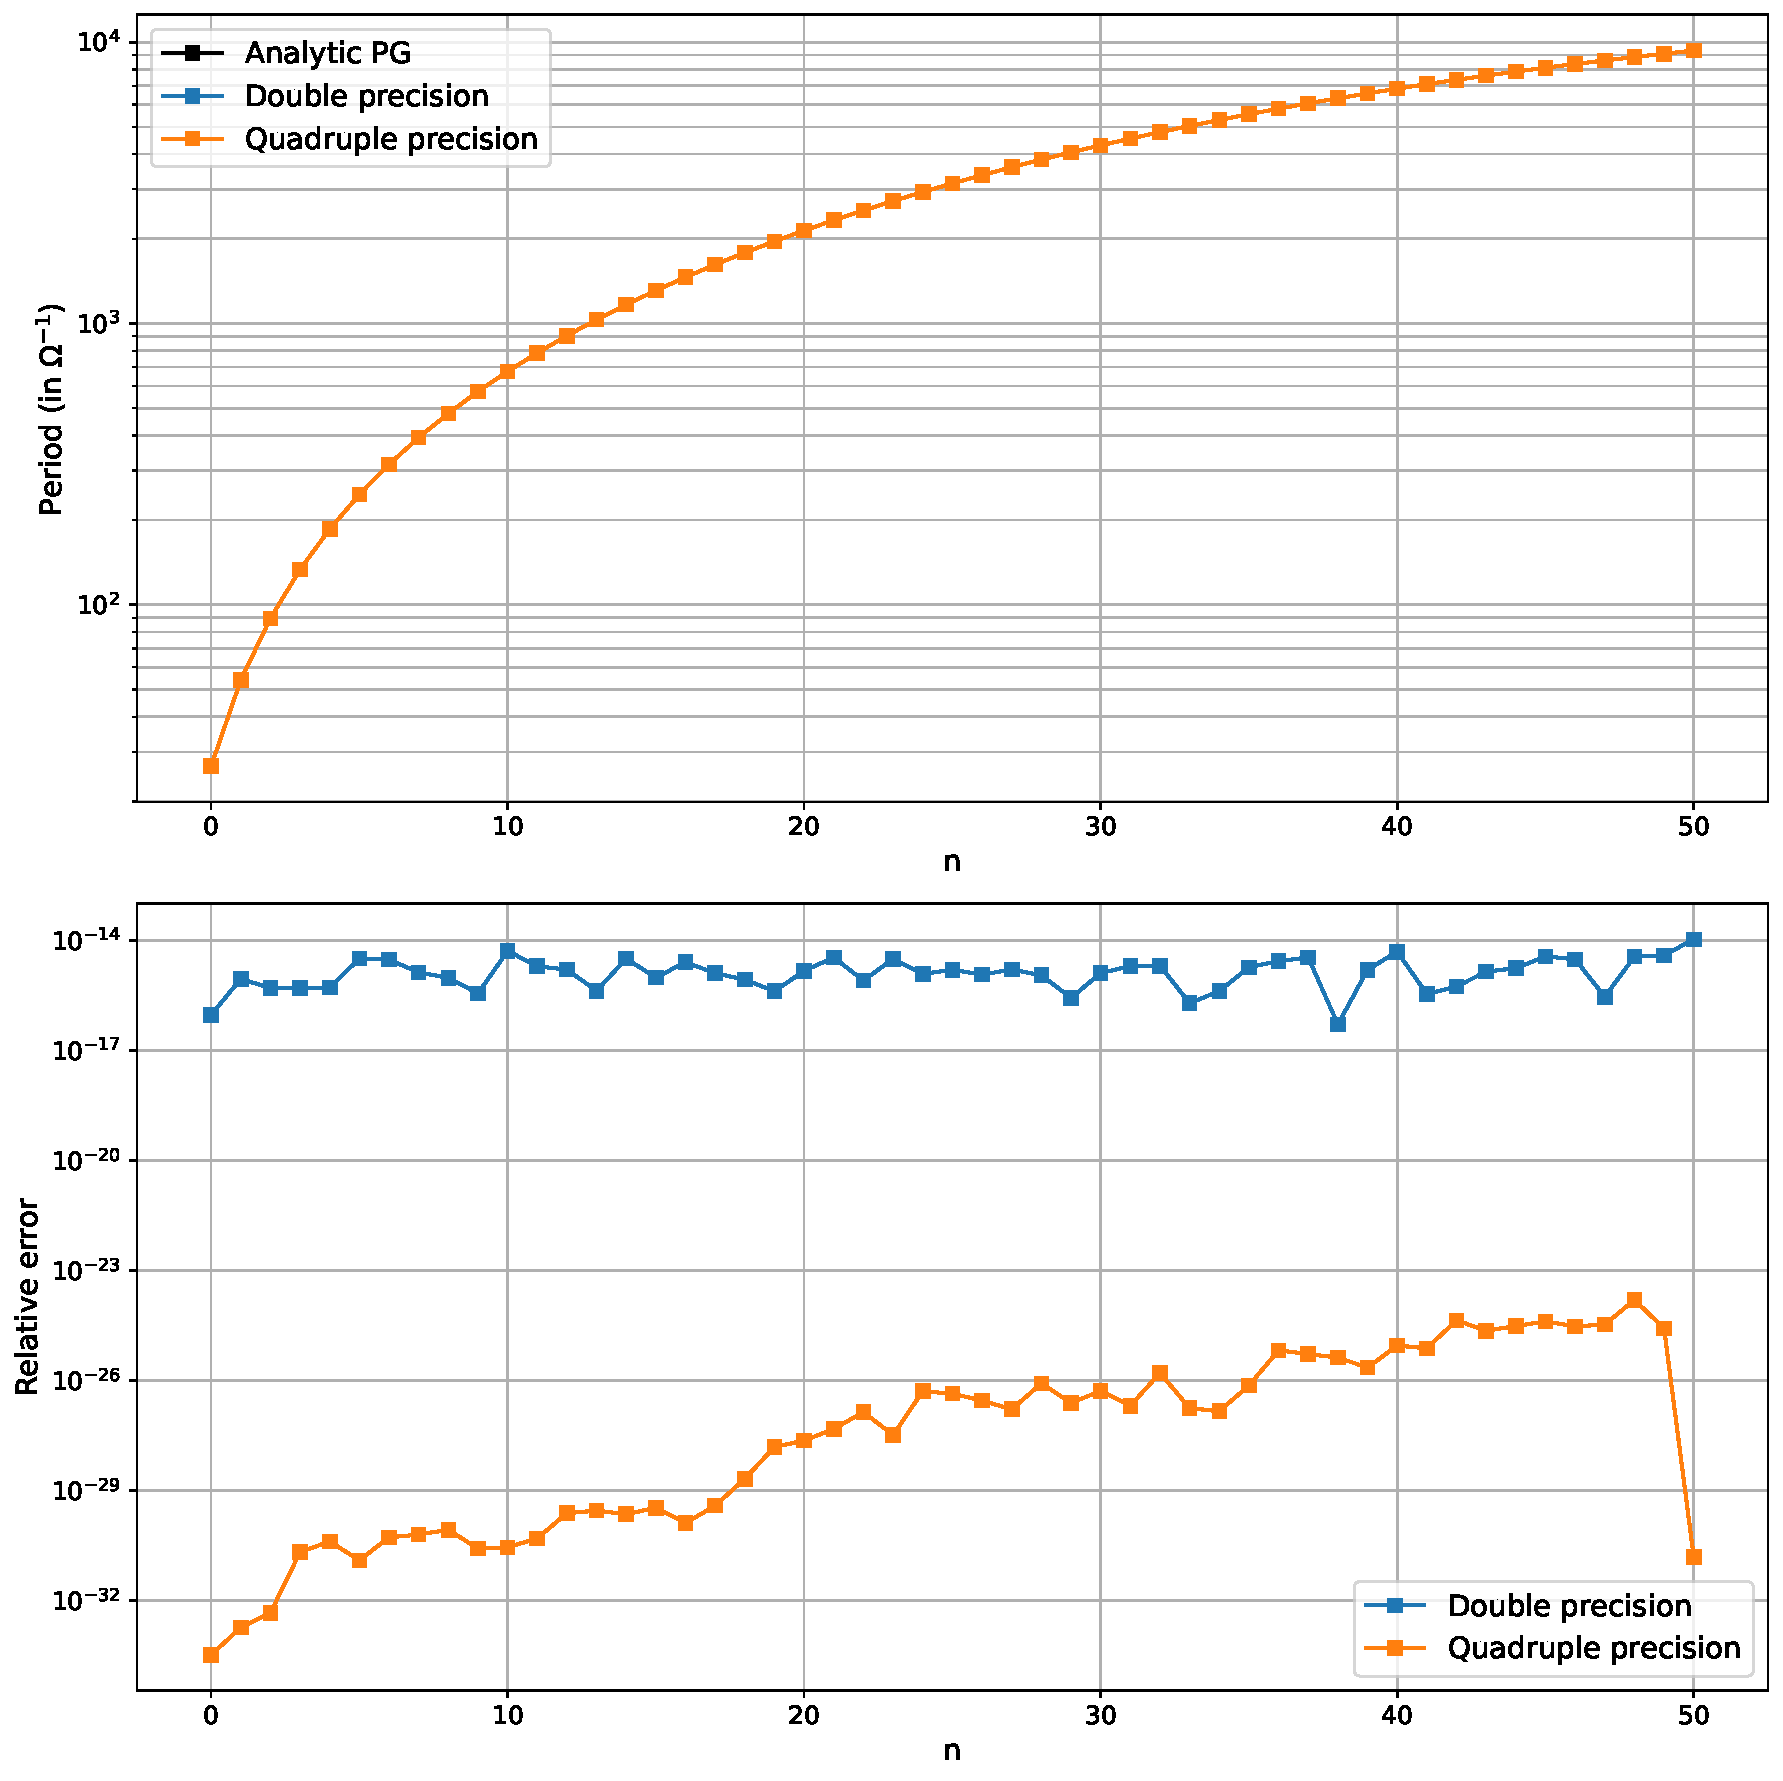
\includegraphics[width=.8\linewidth]{../../out/eigen/Malkus/Reduced/Analytical_error_precision_fast.pdf}
    \caption{Eigenperiods (upper panel) for $m=3$ fast modes under Malkus background field, solved to double precision and quadruple precision, with their respective errors from the analytical solution (lower panel). Both calculations are done using the reduced system and a truncation level $N=50$.}
\end{figure}

\begin{figure}[htbp]
    \centering
    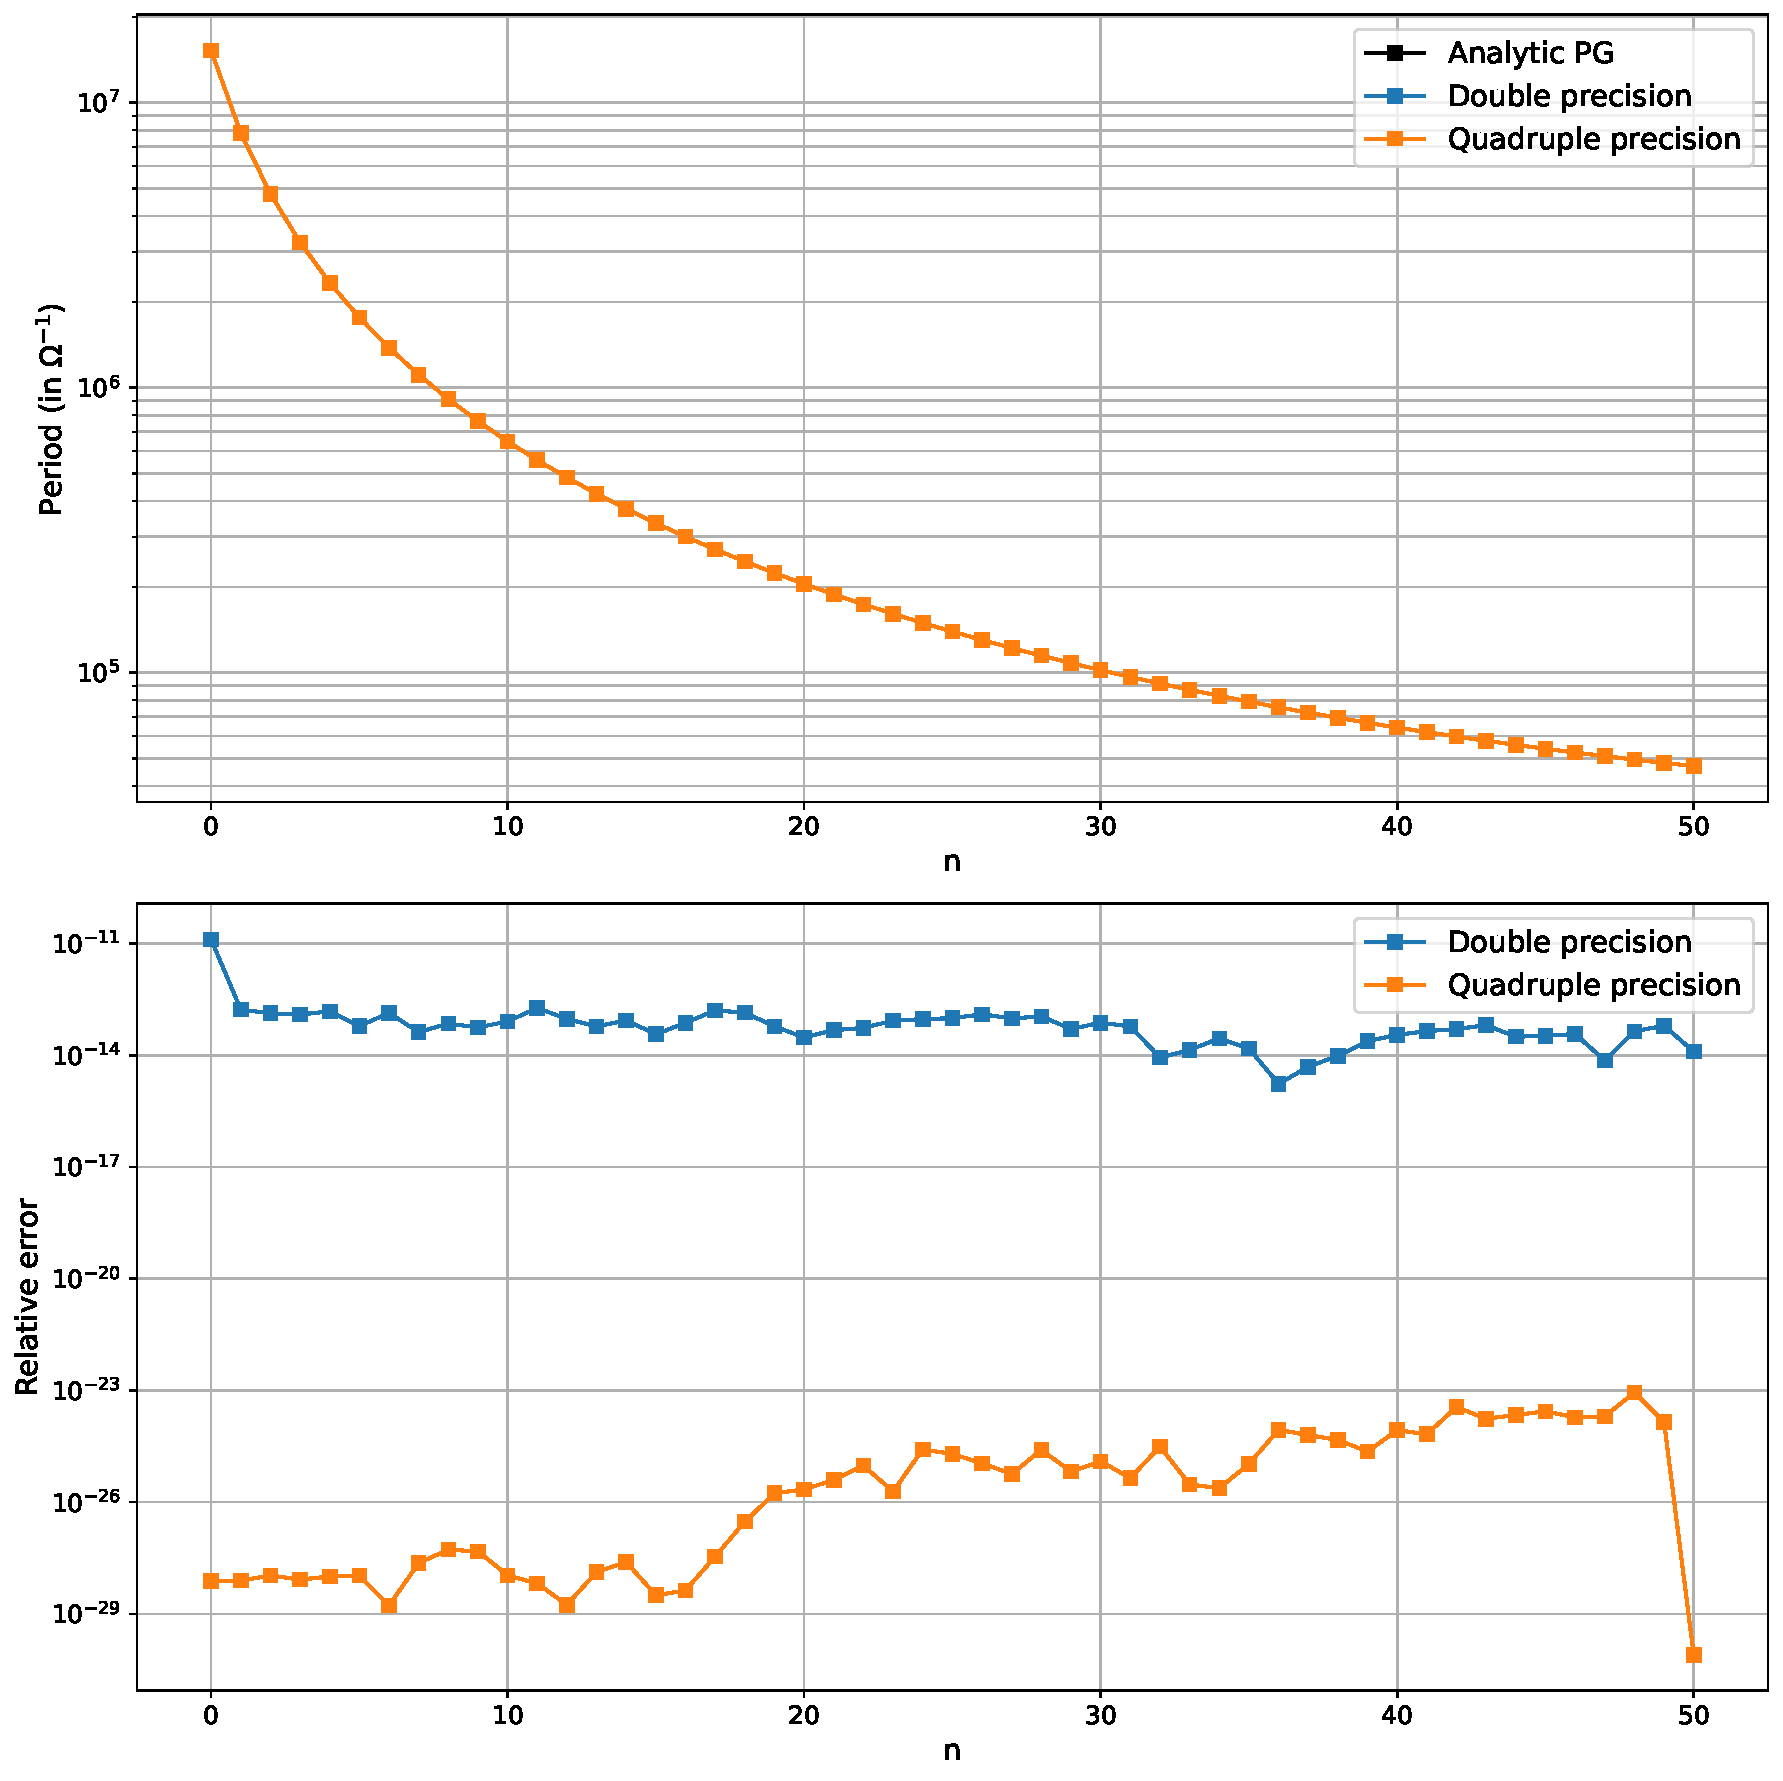
\includegraphics[width=.8\linewidth]{../../out/eigen/Malkus/Reduced/Analytical_error_precision_slow.pdf}
    \caption{Eigenperiods (upper panel) for $m=3$ slow modes under Malkus background field, solved to double precision and quadruple precision, with their respective errors from the analytical solution (lower panel). Both calculations are done using the reduced system and a truncation level $N=50$.}
\end{figure}



\section{Eigenvalue filtering}

Boyd's eigenvalue shift:
\begin{equation}
    \delta_j = \min_{k\in[1, N_2]} \frac{\left|\lambda_j(N_1) - \lambda_k(N_2)\right|}{\sigma_j}
\end{equation}

Maximum trailing rate of exponential convergence:
\begin{equation}
    C_j = \min_{n} \frac{\max_{k\geq n} \log\left|\frac{a_k^{(j)}}{a_n^{(j)}}\right|}{\left|n - n_0^{(j)}\right| + 1}
\end{equation}


\clearpage

\appendix

\chapter{Code design}

\section{Unifined Modelling Language (UML) graphs of the code}

\begin{figure}[ht]
    \centering
    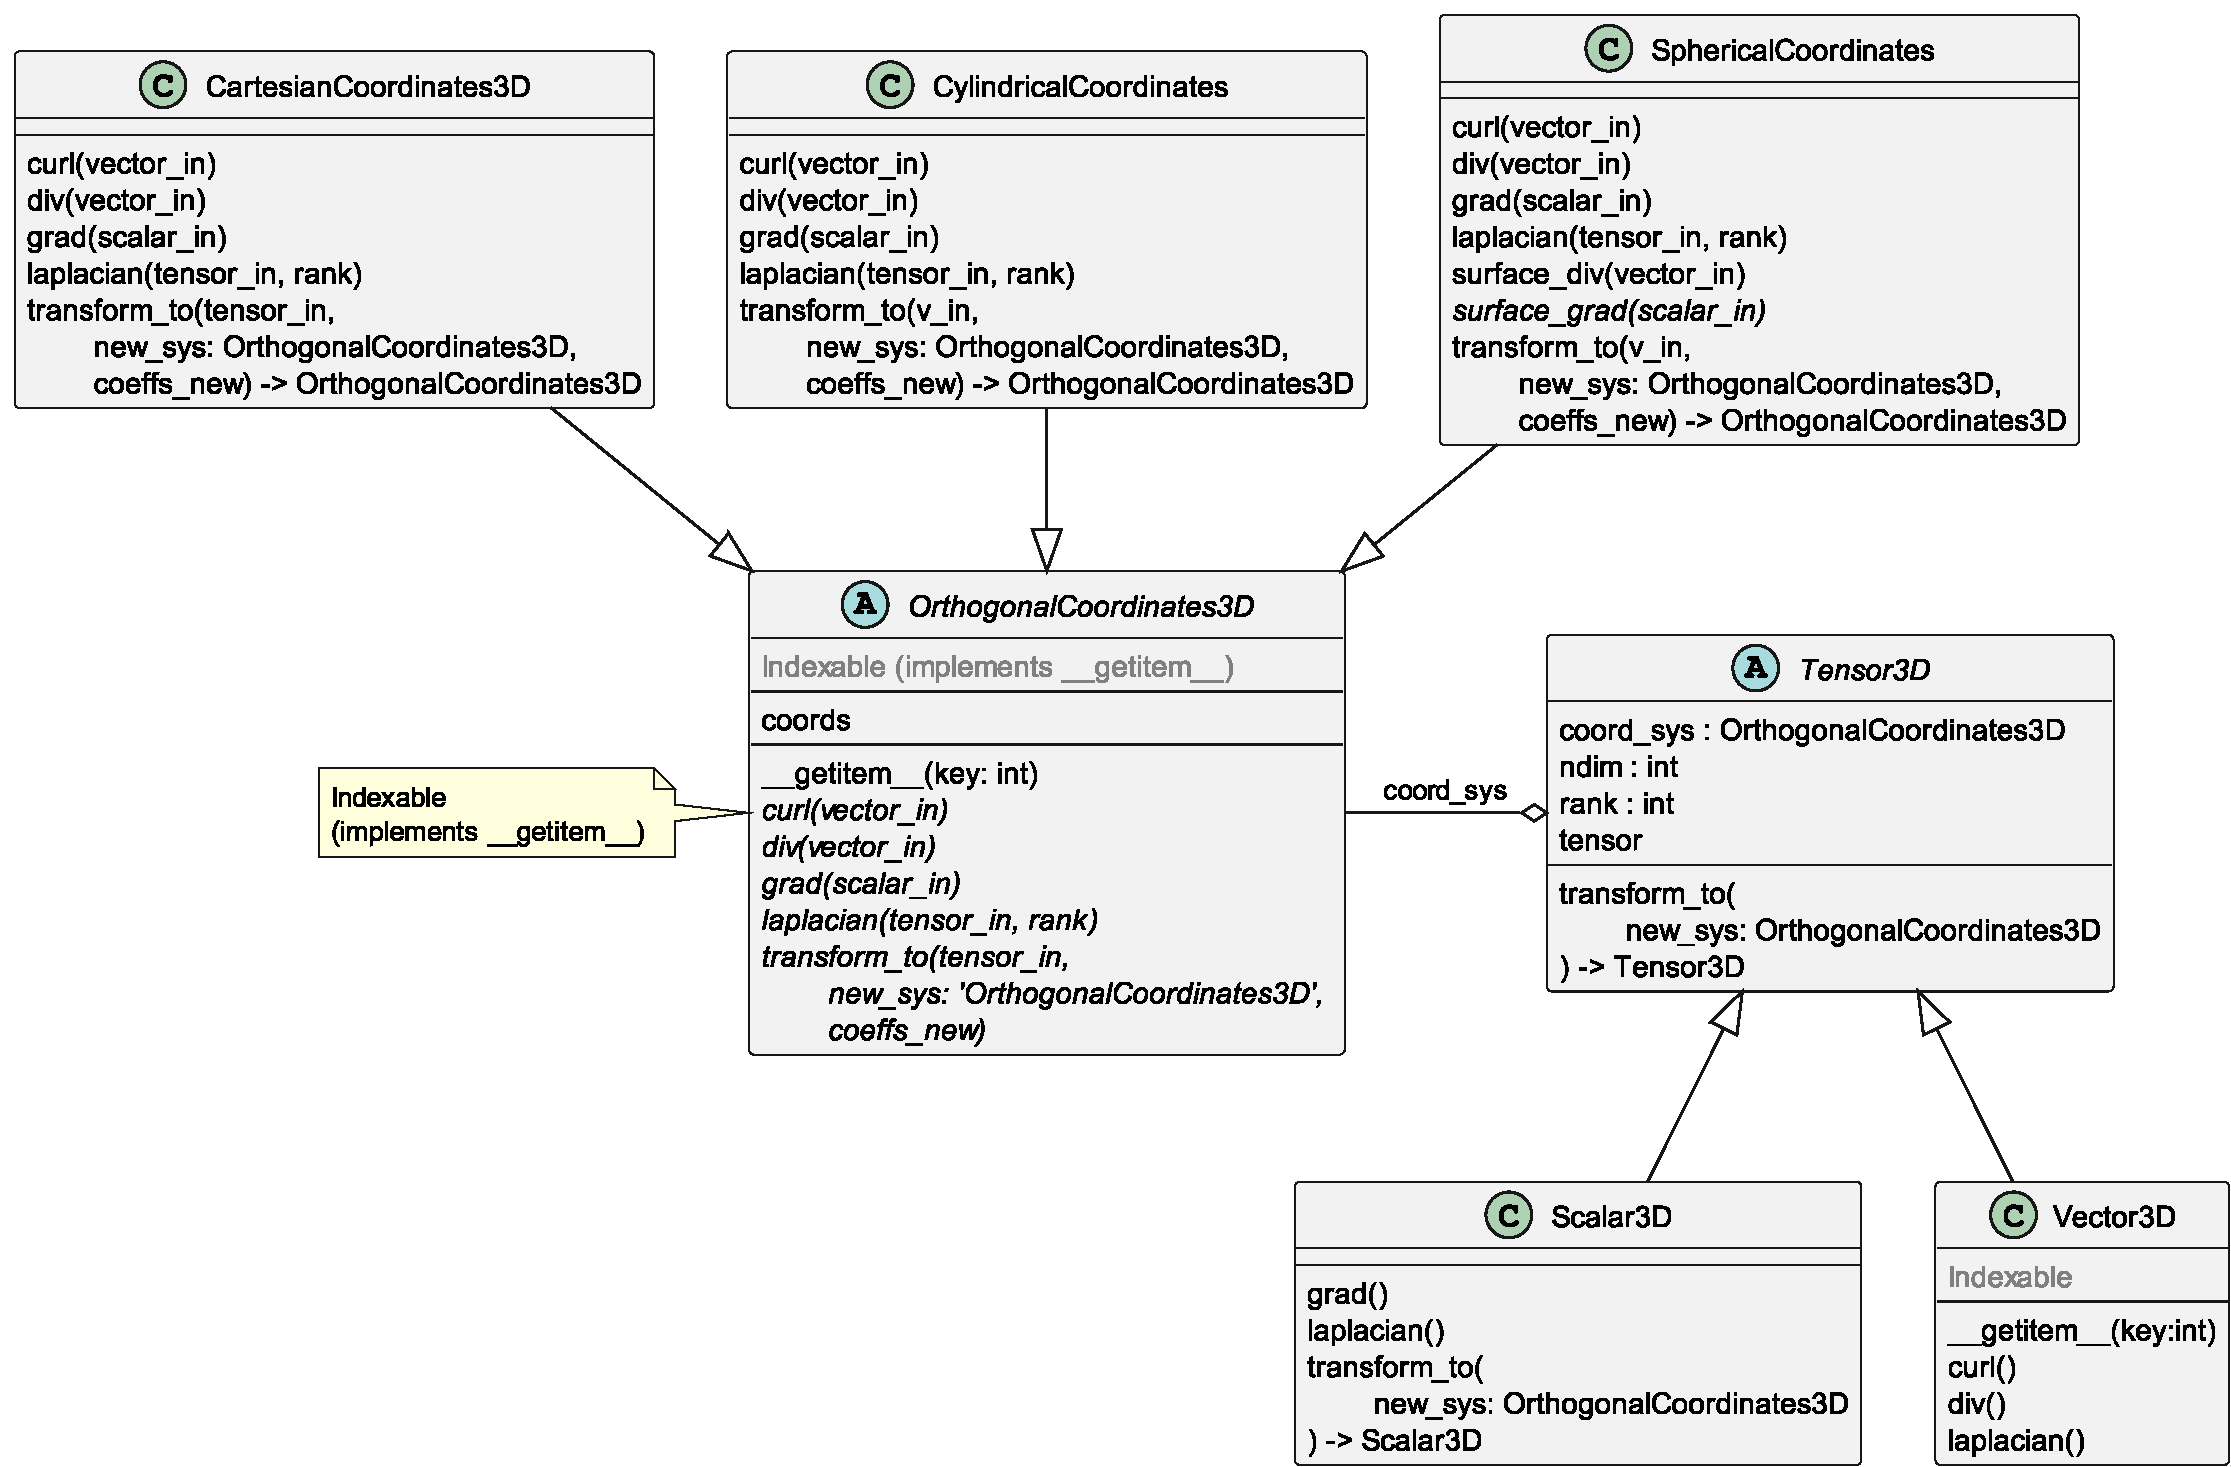
\includegraphics[width=\linewidth]{../Materials/classes_vector_calculus.pdf}
    \caption{Module for supplementary vector operations and calculus.}
\end{figure}


\begin{figure}[ht]
    \centering
    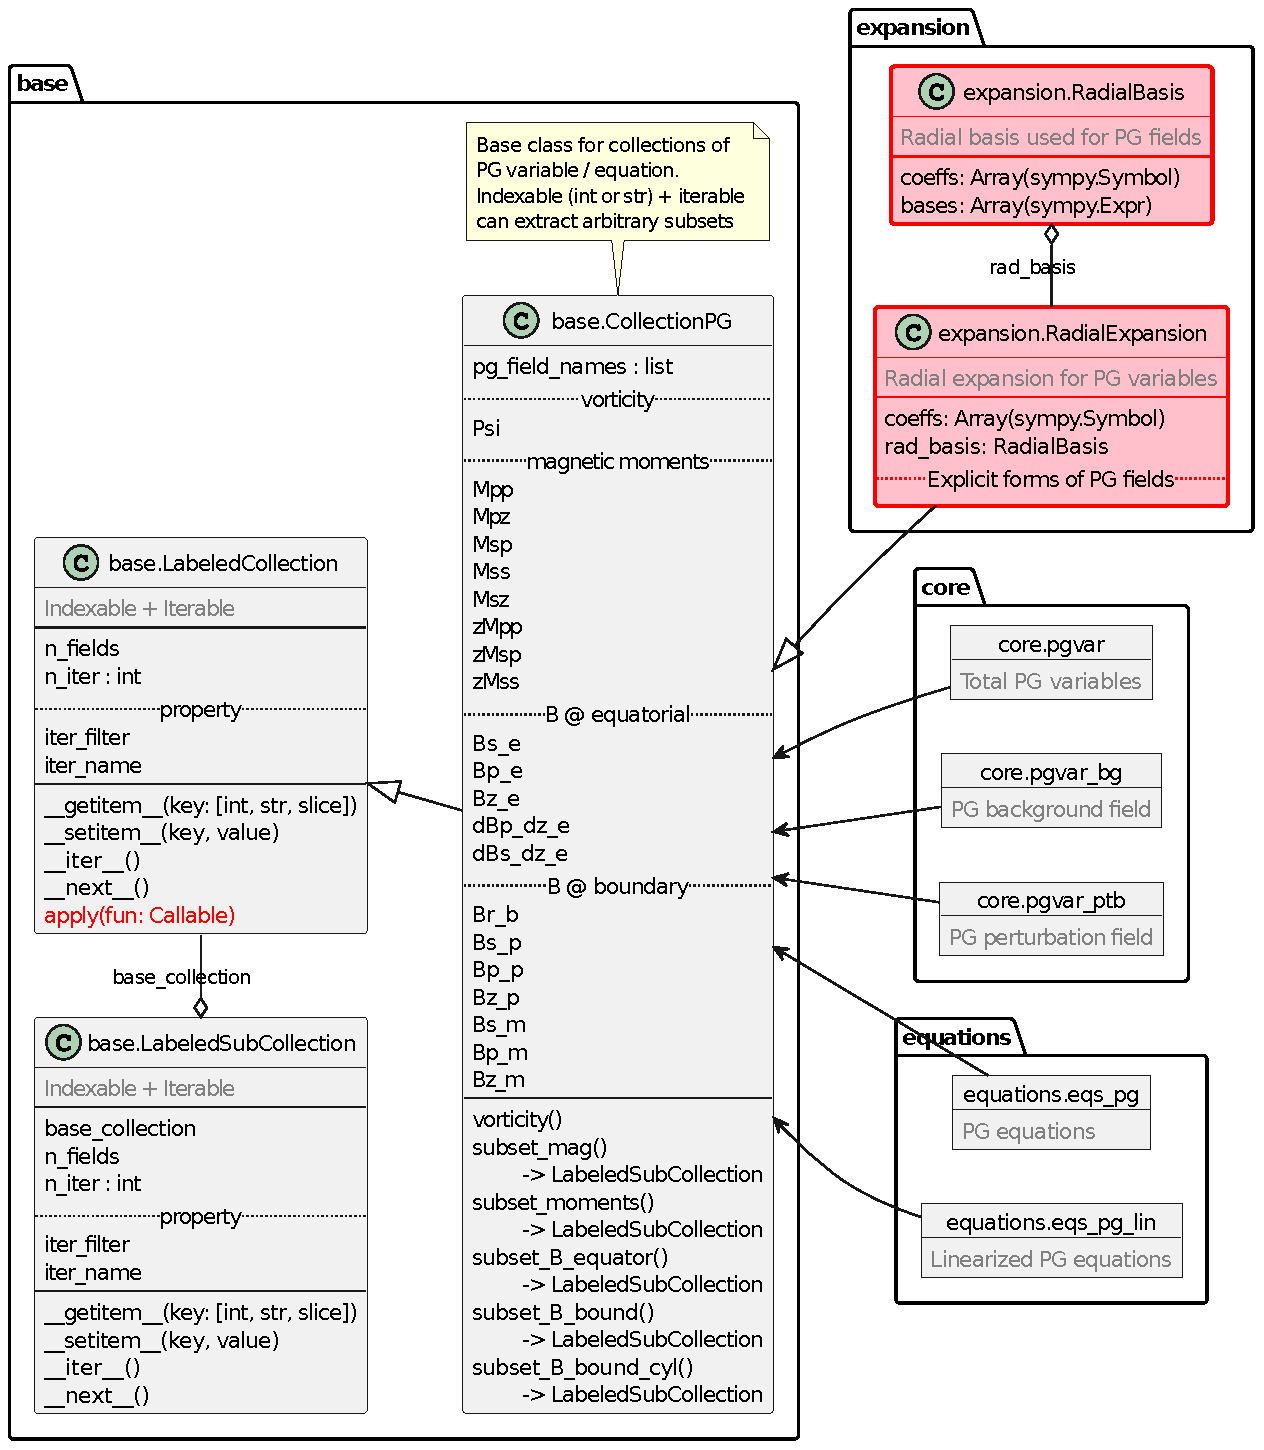
\includegraphics[width=\linewidth]{../Materials/classes_pg_model.pdf}
    \caption{Module PG model. Red items are items to be implemented}
\end{figure}


\clearpage

% [Deprecated][Archived] Derivation of regularity constraints on magnetic moments, following Daria's approach
% \section{Extended expansion for magnetic moments}

The three components of magnetic fields in cylindrical coordinates can be expanded as
\begin{equation}
\begin{aligned}
    B_s &= s g_0 + \sum_{m\neq 0} \left(\lambda_m s^{|m|-1} + g_m s^{|m|+1}\right) e^{im\phi}, \\ 
    B_\phi &= s h_0 + \sum_{m\neq 0} \left(i \sgn(m) \lambda_m s^{|m|-1} + h_m s^{|m|+1}\right) e^{im\phi}, \\ 
    B_z &= f_0 + \sum_{m\neq 0} f_m s^{|m|} e^{im\phi},
\end{aligned}
\end{equation}
where the regularity constraints from \textcite{lewis_physical_1990} is used. The coefficients are regular functions of $z$ and $s$, and according to symmetry arguments they are even functions of $s$. Therefore, the explicit dependency can be written as
\begin{equation}
    \lambda_m = \lambda_m(z),\quad g_m = g_m(z, s^2),\quad h_m = h_m(z, s^2),\quad f_m = f_m(z, s^2).
\end{equation}
Note for the quantities to be real, the Fourier coefficients should satisfy
\[
    \lambda_{-m}^* = \lambda_m,\quad g_{-m}^* = g_m,\quad h_{-m}^* = h_m,\quad f_{-m}^* = f_m.
\]
Here the asterik superscript $\cdot^*$ denotes complex conjugate. Of course, a corollary is that the zero-azimuthal-wavenumber terms, $g_0, h_0, f_0 \in \mathbb{R}$. Also, $(i \sgn(-m) \lambda_{-m})^* = i\sgn(m) \lambda_m$ is automatically satisified. Therefore, $c_m c_{-m} = c_m c_m^* = |c_m|^2$ for any coefficients.

\subsection{Magnetic moment $B_s^2$ rederived}

\begin{equation}
\begin{aligned}
    B_s^2 &= s^2 g_0^2 + 2s g_0 \sum_{m\neq 0} \left(\lambda_m s^{|m|-1} + g_m s^{|m|+1}\right) e^{im\phi} \\
    &\quad + \sum_{n,k\neq 0} \left(\lambda_n \lambda_k s^{|n|+|k|-2} + \left(\lambda_n g_k + g_n \lambda_k\right) s^{|n| + |k|} + g_n g_k s^{|n|+|k|+2} \right) e^{i(n+k)\phi} \\ 
    &= \left\{g_0^2 s^2 + \sum_{n\neq 0} \left[\lambda_n \lambda_{-n} s^{2|n|-2} + \left(\lambda_n g_{-n} + g_n \lambda_{-n}\right) s^{2|n|} + g_n g_{-n}  s^{2|n|+ 2} \right]\right\} \\ 
    &\quad + \sum_{m\neq 0} e^{im\phi} \Bigg\{2g_0 \lambda_m s^{|m|} + 2 g_0 g_m s^{|m|+2} \\
    &\qquad + \sum_{n\neq 0, m} \left[\lambda_n\lambda_{m-n} s^{|n|+|n-m|-2} + \left(\lambda_n g_{m-n} + g_n \lambda_{m-n}\right)s^{|n|+|n-m|} + g_n g_{m-n} s^{|n|+|n-m|+2}\right] \Bigg\}
    % &= \left\{ g_0^2 s^2 + \sum_{n\neq 0} \left[|\lambda_n|^2 s^{2|n|-2} + \left(\lambda_n \overline{g_n} + g_n \overline{\lambda_n}\right)s^{2|n|} + |g_n|^2 s^{2|n|+2}\right]\right\} + \sum_{m\neq 0} e^{im\phi} \Bigg\{ 2s^{|m|} \left(g_0 \lambda_m + g_0 g_m s^2\right)\\
    % &\qquad + \sum_{n\neq 0, m} \left[\lambda_n\lambda_{m-n} s^{|n|+|n-m|-2} + \left(\lambda_n g_{m-n} + g_n \lambda_{m-n}\right)s^{|n|+|n-m|} + g_n g_{m-n} s^{|n|+|n-m|+2}\right] \Bigg\}
\end{aligned}
\end{equation}
There is further simplification that can be performed on the final term. By dividing the nontrivial azimuthal wavenumbers into positive and negative branches, the contribution from the cross-terms is apparently written as
\begin{equation}
\begin{aligned}
    &\sum_{m > 0} e^{im\phi} \left[2 g_0 \lambda_m s^m + 2g_0 g_m s^{m+2}\right] + \sum_{m<0} e^{im\phi} \left[2 g_0 \lambda_m s^{-m} + 2g_0 g_m s^{-m+2}\right] \\ 
    =& \sum_{m > 0} e^{im\phi} \left[2 g_0 \lambda_m s^m + 2g_0 g_m s^{m+2}\right] +\sum_{m>0} e^{-im\phi} \left[2 g_0 \lambda_{-m} s^m + 2g_0 g_{-m} s^{m+2}\right] \\
    =& \sum_{m > 0} e^{im\phi} \left[2 g_0 \lambda_m s^m + 2g_0 g_m s^{m+2}\right] +\sum_{m>0} e^{-im\phi} \left[2 g_0 \lambda_m^* s^m + 2g_0 g_m^* s^{m+2}\right]
\end{aligned}
\end{equation}
For the second contribution, we can further separate the inner summation into three parts: the part where $n$ and $m-n$ have the same sign, the part where $n > 0$ and $m-n < 0$, and the part where $n < 0$ and $m-n > 0$. Let us consider the case when $m>0$ first.
\begin{equation}
\begin{aligned}
    &\sum_{n\neq 0, m} \left[\lambda_n\lambda_{m-n} s^{|n|+|n-m|-2} + \left(\lambda_n g_{m-n} + g_n \lambda_{m-n}\right)s^{|n|+|n-m|} + g_n g_{m-n} s^{|n|+|n-m|+2}\right] \\ 
    =& \left(\sum_{n < 0} + \sum_{0 < n < m} + \sum_{n > m}\right) \left[\lambda_n\lambda_{m-n} s^{|n|+|n-m|-2} + \left(\lambda_n g_{m-n} + g_n \lambda_{m-n}\right)s^{|n|+|n-m|} + g_n g_{m-n} s^{|n|+|n-m|+2}\right] \\ 
    =& \sum_{n < 0} \left[\lambda_n\lambda_{m-n} s^{m-2n-2} + \left(\lambda_n g_{m-n} + g_n \lambda_{m-n}\right)s^{m-2n} + g_n g_{m-n} s^{m-2n+2}\right] \\ 
    &+ \sum_{0<n<m} \left[\lambda_n\lambda_{m-n} s^{m-2} + \left(\lambda_n g_{m-n} + g_n \lambda_{m-n}\right)s^{m} + g_n g_{m-n} s^{m+2}\right] \\ 
    &+ \sum_{n > m} \left[\lambda_n\lambda_{m-n} s^{2n-m-2} + \left(\lambda_n g_{m-n} + g_n \lambda_{m-n}\right)s^{2n-m} + g_n g_{m-n} s^{2n-m+2}\right] \\ 
    =& \sum_{0<n<m} \left[\lambda_n\lambda_{m-n} s^{m-2} + \left(\lambda_n g_{m-n} + g_n \lambda_{m-n}\right)s^{m} + g_n g_{m-n} s^{m+2}\right] \\ 
    &+ \sum_{n > 0} \left[\lambda_{-n}\lambda_{m+n} s^{m+2n-2} + \left(\lambda_{-n} g_{m+n} + g_{-n} \lambda_{m+n}\right)s^{m+2n} + g_{-n} g_{m+n} s^{m+2n+2}\right] \\ 
    &+ \sum_{n > 0} \left[\lambda_{n+m}\lambda_{-n} s^{2n+m-2} + \left(\lambda_{n+m} g_{-n} + g_{n+m} \lambda_{-n}\right)s^{2n+m} + g_{n+m} g_{-n} s^{2n+m+2}\right] \\ 
    =& \sum_{0<n<m} \left[\lambda_n\lambda_{m-n} s^{m-2} + \left(\lambda_n g_{m-n} + g_n \lambda_{m-n}\right)s^{m} + g_n g_{m-n} s^{m+2}\right] \\ 
    &+ 2\sum_{n > 0} \left[\lambda_{n+m} \lambda_n^* s^{m+2n-2} + \left(\lambda_{n+m} g_n^* + g_{n+m} \lambda_n^*\right) s^{m+2n} + g_{n+m} g_n^* s^{m+2n+2}\right]
\end{aligned}
\end{equation}
The symmetry of $n$ and $m-n$ enables collapsing the two summations into one.
This way it is even possible to write explicitly the coefficient of $e^{im\phi}$ as an expansion of $s$. For $m > 0$, the Fourier coefficient for $B_s^2$ therefore reads
\begin{equation}
\begin{aligned}
    &s^{m-2} \sum_{0<n<m} \lambda_n \lambda_{m-n} + s^m \left(2g_0 \lambda_m + \sum_{0<n<m} (\lambda_n g_{m-n} + g_n \lambda_{m-n}) + 2 \lambda_{m+1} \lambda_1^*\right) \\ 
    +& s^{m+2} \left(2g_0 g_m + \sum_{0 < n < m} g_n g_{m-n} + 2 \left(\lambda_{m+2} \lambda_2^* + \lambda_{m+1} g_1^* + g_{m+1} \lambda_1^*\right) \right) \\
    +& \sum_{n > 1} s^{m+2n} \left[\lambda_{m+n+1} \lambda_{n+1}^* + \lambda_{m+n} g_n^* + g_{m+n} \lambda_n^* + g_{m+n-1} g_{n-1}^*\right].
\end{aligned}
\end{equation}
The situation for $m < 0$ is fairly similar, and can be straightforwardly obtained again using the complex conjugate property of the Fourier coefficients of real fields,
\begin{equation}
    \begin{aligned}
        &s^{|m|-2} \sum_{0<n<|m|} (\lambda_n \lambda_{|m|-n})^* + s^{|m|} \left(2g_0 \lambda_{|m|}^* + \sum_{0<n<|m|} ((\lambda_n g_{|m|-n})^* + (g_n \lambda_{|m|-n})^*) + 2 \lambda_{|m|+1}^* \lambda_1\right) \\ 
        +& s^{|m|+2} \left(2g_0 g_{|m|}^* + \sum_{0 < n < |m|} (g_n g_{|m|-n})^* + 2 \left(\lambda_{|m|+2}^* \lambda_2 + \lambda_{|m|+1}^* g_1 + g_{|m|+1}^* \lambda_1\right) \right) \\
        +& \sum_{n > 1} s^{|m|+2n} \left[\lambda_{|m|+n+1}^* \lambda_{n+1} + \lambda_{|m|+n}^* g_n + g_{|m|+n}^* \lambda_n + g_{|m|+n-1}^* g_{n-1}\right].
    \end{aligned}
\end{equation}
The full expansion can then be written in terms of the Fourier coefficients of $B_s$ as
\begin{equation}
\begin{aligned}
    B_s^2 &= \left\{2|\lambda_1|^2 + s^2\left(g_0^2 + 2|\lambda_2|^2 + 4 \Re[\lambda_1 g_1^*]\right) + 2\sum_{n>1} s^{2n} \left(|\lambda_{n+1}|^2 + |g_{n-1}|^2 + 2 \Re[\lambda_n g_n^*]\right)\right\} \\
    + \sum_{m>0} &e^{im\phi} \Bigg\{s^{m-2} \sum_{0<n<m} \lambda_n \lambda_{m-n} + s^m \left(2g_0 \lambda_m + \sum_{0<n<m} (\lambda_n g_{m-n} + g_n \lambda_{m-n}) + 2 \lambda_{m+1} \lambda_1^* \right) \\ 
    +& s^{m+2} \left(2g_0 g_m + \sum_{0 < n < m} g_n g_{m-n} + 2 \left(\lambda_{m+2} \lambda_2^* + \lambda_{m+1} g_1^* + g_{m+1} \lambda_1^*\right) \right) \\
    +& \sum_{n > 1} s^{m+2n} \left[\lambda_{m+n+1} \lambda_{n+1}^* + \lambda_{m+n} g_n^* + g_{m+n} \lambda_n^* + g_{m+n-1} g_{n-1}^* \right]\Bigg\} + \sum_{m<0} e^{im\phi} \left(\cdots\right).
\end{aligned}
\end{equation}
We therefore recover the asymptotic behaviour at $s=0$ for $B_s^2$,
\begin{equation}
\begin{aligned}
    \left(B_s^2\right)_{m=0} &= 2 |\lambda_1|^2 + O(s^2) \\ 
    \left(B_s^2\right)_{|m|=1} &= 2s \left(g_0 \lambda_1 + \lambda_{2} \lambda_1^*\right) e^{i\phi} + 2s \left(g_0 \lambda_1^* + \lambda_{2}^* \lambda_1\right) e^{-i\phi} + O(s^3) \\ 
    &= 2s \left[\left(2g_0 \lambda_1^R + \lambda_2^R \lambda_1^R + \lambda_2^I \lambda_1^I\right)\cos\phi - \left(2g_0 \lambda_1^I + \lambda_2^I \lambda_1^R - \lambda_2^R \lambda_1^I \right) \sin\phi\right] + O(s^3) \\
    \left(B_s^2\right)_{|m|>1} &= s^{|m|-2} \sum_{0 < n < |m|} \left(\lambda_n \lambda_{|m|-n} e^{i|m|\phi} + \lambda_n^* \lambda_{|m|-n}^* e^{-i|m|\phi}\right) + O\left(s^{|m|}\right) \\ 
    = s^{|m|-2} &\sum_{0 < n < |m|} \left[ \left(\lambda_n^R \lambda_{|m|-n}^R - \lambda_n^I \lambda_{|m|-n}^I\right) \cos (|m|\phi) - \left(\lambda_n^R \lambda_{|m|-n}^I + \lambda_n^I \lambda_{|m|-n}^R\right) \sin(|m|\phi)\right] + O(s^{|m|})
\end{aligned}
\end{equation}
Apart from a prefactor, this is the same as in \textcite{holdenried-chernoff_long_2021} for $|m|\neq 1$. For $|m|=1$, the contribution from the cross-term $g_0$ seems to be missing in Daria's dissertation. The summation $\sum_{n+k=m}$ (in \cite{holdenried-chernoff_long_2021}) is also misleading; it should technically be constrained to positive $n$ and $k$, so the summation is actually not an infinite sum. That being said, the leading order behaviour in $s$ is correct. The later analysis on the integral in $z$ is also not affected by this discrepancy.

\subsection{General Fourier expansion formulae for moments}

Let two vector components be expressed by
\[
    B_a = s a_0^+ + \sum_{m\neq 0} e^{im\phi} \left(a_m^- s^{|m|-1} + a_m^+ s^{|m|+1} \right),\quad
    B_b = s b_0^+ + \sum_{m\neq 0} e^{im\phi} \left(b_m^- s^{|m|-1} + b_m^+ s^{|m|+1} \right)
\]
The expression applies to either of the two horizontal components of the magnetic fields in cylindrical coordinates. Using the same method, without assuming the complex conjugate property of the Fourier coefficients, we can write
\begin{equation}
\begin{aligned}
    B_a B_b =& \bigg\{\left(a_1^- b_{-1}^- + a_{-1}^- b_1^-\right) + s^2 \left[a_0^+ b_0^+ + \left(a_2^- b_{-2}^- + a_{-2}^- b_2^-\right) + \left(a_1^- b_{-1}^+ + a_{1}^+ b_{-1}^- + a_{-1}^- b_{1}^+ + a_{-1}^+ b_1^-\right)\right]\\
    + \sum_{n > 1}& s^{2n} \left[\left(a_{n+1}^- b_{-n-1}^- + a_{-n-1}^- b_{n+1}^-\right) + \left(a_n^- b_{-n}^+ + a_{n}^+ b_{-n}^- + a_{-n}^- b_{n}^+ + a_{-n}^+ b_n^-\right) + \left(a_{n-1}^+ b_{1-n}^+ + a_{1-n}^+ b_{n-1}^+\right) \right]\bigg\} \\ 
    +\sum_{m > 0} e^{im\phi}& \Bigg\{ s^{m-2} \sum_{0\leq n\leq m} a_n^- b_{m-n}^- + s^m \left[a_{-1}^- b_{m+1}^- + a_{m+1}^- b_{-1}^- + \sum_{0\leq n\leq m} \left(a_n^- b_{m-n}^+ + a_n^+ b_{m-n}^-\right)\right] \\
    + s^{m+2}& \left[a_{-2}^- b_{m+2}^- + a_{m+2}^- b_{-2}^- + a_{m+1}^- b_{-1}^+ + a_{m+1}^+ b_{-1}^- + a_{-1}^+ b_{m+1}^- + a_{-1}^- b_{m+1}^+ + \sum_{0\leq n\leq m} a_n^+ b_{m-n}^+ \right] \\
    + s^m& \sum_{n \geq 2} s^{2n} \bigg[\left(a_{-n-1}^- b_{m+n+1}^- + a_{m+n+1}^- b_{-n-1}^-\right) + \left(a_{-n}^{-} b_{m+n}^+ + a_{-n}^{+} b_{m+n}^- + a_{m+n}^{-} b_{-n}^+ + a_{m+n}^{+} b_{-n}^-\right) \\
    &\quad + \left(a_{-n+1}^+b_{m+n-1}^+ + a_{-n+1}^{-} b_{m+n-1}^+\right)\bigg] \Bigg\} \\ 
    +\sum_{m < 0} e^{im\phi}& \Bigg\{ s^{|m|-2} \sum_{m\leq n\leq 0} a_n^- b_{m-n}^- + s^{|m|} \left[a_{1}^- b_{m-1}^- + a_{m-1}^- b_{1}^- + \sum_{m\leq n\leq 0} \left(a_n^- b_{m-n}^+ + a_n^+ b_{m-n}^-\right)\right] \\
    + s^{|m|+2}& \left[a_{2}^- b_{m-2}^- + a_{m-2}^- b_{2}^- + a_{m-1}^- b_{1}^+ + a_{m-1}^+ b_{1}^- + a_{1}^+ b_{m-1}^- + a_{1}^- b_{m-1}^+ + \sum_{m\leq n\leq 0} a_n^+ b_{m-n}^+ \right] \\
    + s^{|m|} & \sum_{n \geq 2} s^{2n} \bigg[\left(a_{n+1}^- b_{m-n-1}^- + a_{m-n-1}^- b_{n+1}^-\right) + \left(a_{n}^{-} b_{m-n}^+ + a_{n}^{+} b_{m-n}^- + a_{m-n}^{-} b_{n}^+ + a_{m-n}^{+} b_{n}^-\right) \\
    &\quad + \left(a_{n-1}^+b_{m-n+1}^+ + a_{n-1}^{-} b_{m-n+1}^+\right)\bigg] \Bigg\}
\end{aligned}
\end{equation}
Here we already used the property $a_0^- = b_0^- = 0$ to add trivial terms, and merged cross terms involving $a_0^+$, $b_0^+$ in the summation $\sum_{0\leq n \leq m}$ or $\sum_{m\leq n \leq 0}$. Plugging in $a_{n}^- = b_n^- = \lambda_n$ and $a_n^+ = b_n^+ = g_n$, and assuming $\lambda_{-n}^* = \lambda_n$, $g_{-n}^* = g_n$, one can easily verify that the equation leads to the expansion for $B_s^2$. The lowest order term in $s$ for arbitrary Fourier coefficient is also readily given as a corollary:
\begin{equation}
\begin{aligned}
    \left(B_a B_b\right)_{m=0} &= a_1^- b_{-1}^- + a_{-1}^- b_{1}^- + O\left(s^2\right) \\ 
    \left(B_a B_b\right)_{|m|=1} &= s e^{+i\phi}\left[a_{-1}^- b_{2}^- + a_{2}^- b_{-1}^- + a_1^- b_0^+ + a_0^+ b_1^-\right]\\
    &+ s e^{-i\phi}\left[a_{1}^- b_{-2}^- + a_{-2}^- b_{1}^- + a_{-1}^- b_0^+ + a_0^+ b_{-1}^-\right] + O\left(s^3\right) \\ 
    \left(B_a B_b\right)_{|m|>1} &= s^{|m|-2} e^{+i|m|\phi} \sum_{0\leq n \leq |m|} a_n^- b_{|m|-n}^- \\
    &+ s^{|m|-2} e^{-i|m|\phi} \sum_{-|m| \leq n \leq 0} a_n^- b_{-|m|-n}^- + O\left(s^{|m|}\right)
\end{aligned}
\end{equation}
On the other hand, a scalar that is regular in cylindrical coordinates takes the form
\begin{equation}
F = \sum_{m\in \mathbb{Z}} f_m s^{|m|} e^{im\phi} = f_0 + \sum_{m\neq 0} f_m s^{|m|} e^{im\phi}
\end{equation}
This applies to $B_z$. Its moment with any equatorial component takes the form
\begin{equation}
\begin{aligned}
    F B_a &= s f_0 a_0^+ + \sum_{n\neq 0} \left(f_{-n} a_n^- s^{2|n|-1} + f_{-n} a_n^+ s^{2|n|+1}\right) + \sum_{m\neq 0} \left[f_0 a_{m}^- s^{|m|-1} + \left(f_0 a_m^+ + f_m a_0^+\right) s^{|m|+1}\right] e^{im\phi} \\
    &+ \sum_{m > 0} e^{im\phi} \Bigg[s^{m-1} \sum_{0<n<m} f_{m-n} a_n^- + s^{m+1} \sum_{0<n<m} f_{m-n} a_n^+ \\
    &+\quad  \sum_{n>0} \left(\left(f_{-n} a_{m+n}^- + f_{m+n} a_{-n}^- \right) s^{m+2n-1} + \left(f_{-n} a_{m+n}^+ + f_{m+n} a_{-n}^+ \right) s^{m+2n+1} \right) \Bigg] \\
    &+ \sum_{m < 0} e^{im\phi} \Bigg[s^{|m|-1} \sum_{m<n<0} f_{m-n} a_n^- + s^{m+1} \sum_{m<n<0} f_{m-n} a_n^+ \\
    &+\quad  \sum_{n>0} \left(\left(f_{n} a_{m-n}^- + f_{m-n} a_{n}^- \right) s^{|m|+2n-1} + \left(f_{n} a_{m-n}^+ + f_{m-n} a_{n}^+ \right) s^{|m|+2n+1} \right) \Bigg] \\
    F B_a &= s \left(f_0 a_0^+ + f_{-1} a_1^- + f_1 a_{-1}^-\right) + \sum_{n\geq 1} s^{2n+1} \left(f_{-n-1} a_{n+1}^- + f_{n+1} a_{-n-1}^- + f_{-n} a_n^+ + f_n a_{-n}^+ \right) \\
    &+ \sum_{m > 0} e^{im\phi} s^{m-1} \Bigg[ \left(\sum_{0\leq n\leq m} f_{m-n} a_n^-\right) + \left(\sum_{0\leq n\leq m} f_{m-n} a_n^+ + f_{-1}a_{m+1}^- + f_{m+1} a_{-1}^- \right) s^2 \\
    &\qquad + \sum_{n\geq 2} s^{2n} \left(f_{-n} a_{m+n}^- + f_{m+n} a_{-n}^- + f_{1-n} a_{m+n-1}^+ + f_{m+n-1} a_{1-n}^+\right) \Bigg] \\ 
    &+ \sum_{m < 0} e^{im\phi} s^{|m|-1} \Bigg[ \left(\sum_{m\leq n\leq 0} f_{m-n} a_n^-\right) + \left(\sum_{m\leq n\leq 0} f_{m-n} a_n^+ + f_{1}a_{m-1}^- + f_{m-1} a_{1}^- \right) s^2 \\
    &\qquad + \sum_{n\geq 2} s^{2n} \left(f_{n} a_{m-n}^- + f_{m-n} a_{n}^- + f_{n-1} a_{m-n+1}^+ + f_{m-n+1} a_{n-1}^+\right) \Bigg]
\end{aligned}
\end{equation}
The lowest order behaviour in $s$ at different azimuthal wavenumber:
\begin{equation}
\begin{aligned}
    (FB_a)_{m=0} &= s \left(f_0 a_0^+ + f_{-1} a_1^- + f_1 a_{-1}^-\right) + O(s^3) \\ 
    (FB_a)_{m\neq 0} &= s^{|m|-1} \sum_{0\leq n \leq |m|} \left( f_{|m|-n} a_n^- e^{i|m|\phi} + f_{-|m|+n} a_{-n}^- e^{-i|m|\phi}\right) + O(s^{|m|+1}).
\end{aligned}
\end{equation}

\subsection{Axial asymptotic of magnetic moments}

Here I write out the explicit form of the lowest order dependency on $s$ at different azimuthal wavenumber for magnetic moments. For $B_s^2$, we have $a_m^- = b_m^- = \lambda_m$, and $a_m^+ = b_m^+ = g_m$. The asymptotics at $s\rightarrow 0$ are as follows, which have already been derived in the first section:
\begin{equation}
\begin{aligned}
    \left(B_s^2\right)_{m=0} &= 2(\lambda_1 \lambda_{-1}) + O\left(s^2\right) \\ 
    \left(B_s^2\right)_{|m|=1} &= 2 s \left[\left(\lambda_2 \lambda_{-1} + g_0 \lambda_1\right) e^{i\phi} + \left(\lambda_{-2} \lambda_{1} + g_0 \lambda_{-1}\right) e^{-i\phi}\right] + O\left(s^3\right) \\ 
    \left(B_s^2\right)_{|m|>1} &= s^{|m|-2} \left[e^{i|m|\phi} \sum_{0\leq n \leq |m|} \lambda_n \lambda_{|m|-n} + e^{-i|m|\phi} \sum_{-|m|\leq n\leq 0} \lambda_n \lambda_{-|m|-n}\right] + O\left(s^{|m|}\right).
\end{aligned}
\end{equation}
Note that here I didn't assume the complex conjugate property between the positive and the negative wavenumbers. For $B_\phi^2$, we have $a_m^- = b_m^- = i\sgn(m)\lambda_m$, and $a_m^+ = b_m^+ = h_m$. We see that the product $a_m^- b_n^- = \lambda_m \lambda_n$ if $m$ and $n$ have different signs, but $-\lambda_m \lambda_n$ if $m$ and $n$ have the same signs. The asymptotics are then given by
\begin{equation}
    \begin{aligned}
        \left(B_\phi^2\right)_{m=0} &= 2 (\lambda_1 \lambda_{-1}) + O\left(s^2\right) \\ 
        \left(B_\phi^2\right)_{|m|=1} &= 2 s \left[\left(\lambda_2 \lambda_{-1} + i h_0 \lambda_1\right) e^{i\phi} + \left(\lambda_{-2} \lambda_{1} - i h_0 \lambda_{-1}\right) e^{-i\phi}\right] + O\left(s^3\right) \\ 
        \left(B_\phi^2\right)_{|m|>1} &= -s^{|m|-2} \left[e^{i|m|\phi} \sum_{0\leq n \leq |m|} \lambda_n \lambda_{|m|-n} + e^{-i|m|\phi} \sum_{-|m|\leq n\leq 0} \lambda_n \lambda_{-|m|-n}\right] + O\left(s^{|m|}\right).
\end{aligned}
\end{equation}
We see that these expressions already differ from those in \textcite{holdenried-chernoff_long_2021}. These include: a two prefactor difference (present in \cite{holdenried-chernoff_long_2021}, but not here) in $|m| > 1$; summation difference in $|m| > 1$; missing terms for $|m|=1$; and missing imaginary unit for one part of $|m|=1$. Nevertheless, the conclusions seem to be correct: lowest-order $s$-dependencies for $B_s^2$ and $B_\phi^2$ are coupled in $m=0$ and $|m|>1$, with prefactor $+1$ and $-1$, respectively. The coupling is not seen for $|m|=1$.

For $B_s B_\phi$, we plug in $a_m^- = \lambda_m$, $b_m^- = i\sgn(m) \lambda_m$, $a_m^+ = g_m$ and $b_m^+ = h_m$. The asymptotics
\begin{equation}
    \begin{aligned}
        \left(B_s B_\phi\right)_{m=0} &= (-i\lambda_1 \lambda_{-1} + i\lambda_{-1} \lambda_1) + O\left(s^2\right) = O\left(s^2\right) \\ 
        \left(B_s B_\phi\right)_{|m|=1} &= s \left[\left(h_0 \lambda_1 + i g_0 \lambda_1\right) e^{i\phi} + \left(h_0 \lambda_{-1} - i g_0 \lambda_{-1}\right) e^{-i\phi}\right] + O\left(s^3\right) \\ 
        \left(B_s B_\phi\right)_{|m|>1} &= i s^{|m|-2} \left[e^{i|m|\phi} \sum_{0\leq n \leq |m|} \lambda_n \lambda_{|m|-n} - e^{-i|m|\phi} \sum_{-|m|\leq n\leq 0} \lambda_n \lambda_{-|m|-n}\right] + O\left(s^{|m|}\right).
    \end{aligned}
\end{equation}
Thus this moment is coupled to $B_s^2$ and $B_\phi^2$ by a factor $i\sgn(m)$ and $-i\sgn(m)$, respectively. Similar couplings are not apprent for $m=0$ and $|m|=1$.

In the moments $B_z B_s$ and $B_z B_\phi$, $B_z$ is treated as scalar, and we need to use the formula involving one equatorial component and one scalar. Taking $a_{m}^- = \lambda_m$ and $a_m^+ = g_m$, we have 
\begin{equation}
\begin{aligned}
    \left(B_z B_s\right)_{m=0} &= s \left(f_0 g_0 + f_{-1} \lambda_1 + f_1 \lambda_{-1}\right) \\ 
    \left(B_z B_s\right)_{m\neq 0} &= s^{|m|-1} \sum_{0\leq n\leq |m|}\left(f_{|m|-n} \lambda_n e^{i|m|\phi} + f_{-|m|+n} \lambda_{-n} e^{-i|m|\phi}\right) + O\left(s^{|m|+1}\right)
\end{aligned}
\end{equation}
Taking $a_m^- = i\sgn(m)\lambda_m$ and $a_m^+ = h_m$, we have
\begin{equation}
    \begin{aligned}
        \left(B_z B_s\right)_{m=0} &= s \left(f_0 h_0 + i f_{-1} \lambda_1 - i f_1 \lambda_{-1}\right) \\ 
        \left(B_z B_s\right)_{m\neq 0} &= s^{|m|-1} \sum_{0\leq n\leq |m|}\left(i f_{|m|-n} \lambda_n e^{i|m|\phi} - i f_{-|m|+n} \lambda_{-n} e^{-i|m|\phi}\right) + O\left(s^{|m|+1}\right)
    \end{aligned}
\end{equation}
Thus these two moment are coupled in the lowest order of $s$ in $m\neq 0$ by a factor $i\sgn(m)$, while there is probably no such coupling in $m=0$. We can conclude that despite all the discrepancies in intermediate steps, the coupling between the moments are the same between this derivation and \textcite{holdenried-chernoff_long_2021}.

\subsection{Axial integral of moment of Fourier coefficients}

It is unsurprising that the Fourier coefficients for $B_s^2$ (and easily shown for all moments) are always summation of $c_n c_k$, where $c=f, g, h, \lambda$. In other words, \textbf{the Fourier coefficients for the magnetic moments are summations of moments of the Fourier coefficients for the magnetic fields.} In fact, I can write the magnetic moment in the general form
\[
    B_a B_b = \sum_m e^{im\phi} s^{m + \Delta_m^{a,b}} \sum_{k \geq 0} s^{2k} \left(\sum_{p,q\in S_{m,k}} c_p c_q\right).
\]
where $\Delta_m^{a,b}$ determines the correction to the lowest order of $s$ at azimuthal wavenumber $m$ (\textcite{holdenried-chernoff_long_2021} found a more concise expression: $s^{||m|-1|})$, given components $a$ and $b$, and $S_{m,k}$ gives the set of all coefficient pairs to sum over at given azimuthal wavenumber $m$ and radial degree index $k$. Among all these terms, however, the only terms with dependency on $z$ are $c_p c_q$. It follows that the axial integrals are
\[
    \overline{z^n B_a B_b} = \sum_m e^{im\phi} s^{m + \Delta} \sum_{k \geq 0} s^{2k} \sum_{p,q} \overline{z^n c_p c_q},\quad
    \widetilde{z^n B_a B_b} = \sum_m e^{im\phi} s^{m + \Delta} \sum_{k \geq 0} s^{2k} \sum_{p,q} \widetilde{z^n c_p c_q}.
\]
If expanding the coefficients in power series of $z$, 
\[
    c_n (z) = \sum_{p \geq 0} c_n^p z^p
\]
the symmetric axial integral of the moments of coefficients are given by
\begin{equation}
\begin{aligned}
    \overline{z^n c_a c_b} &= \int_{-H}^H z^n c_a c_b \, dz = \sum_{p, q \geq 0} c_a^p c_b^q \int_{-H}^H z^{p + q + n} \, dz \\
    &= \sum_{p,q} c_a^p c_b^q \frac{H^{p+q+n+1} - (-H)^{p+q+n+1}}{p + q + n + 1} 
    = \sum_{k\geq 0} \frac{2H^{2k+1}}{2k+1} \sum_{0\leq p \leq 2k-n} c_m^p c_n^{2k-n-p} \\ 
    &= \sqrt{1-s^2} \sum_{k\geq 0} \frac{2}{2k+1} \sum_{0\leq p \leq 2k-n} c_a^p c_b^{2k-n-p} \left(1-s^2\right)^k \\
    &= 2 \sqrt{1-s^2} \sum_{k\geq \lceil \frac{n}{2} \rceil} \frac{\left(c_a^{p} * c_b^p\right)_{2k-n}}{2k+1} \left(1 - s^2\right)^k \\ 
    &= 2 \left(1 - s^2\right)^{\lceil \frac{n}{2} \rceil + \frac{1}{2}} \sum_{k\geq 0} \frac{\left(c_a^{p} * c_b^p\right)_{2k+2\lceil \frac{n}{2} \rceil-n}}{2k+2\lceil\frac{n}{2}\rceil + 1} \left(1 - s^2\right)^k
\end{aligned}
\end{equation}
where $(c_a^p * c_b^p)_{k} = \sum_{0\leq p \leq k} c_a^p c_b^{k-p}$ is the k-th element of the (non-circular) convolution of the finite-length sequence $c_a^p$ and $c_b^p$, $p=0:k$. The only terms left in the integrands are the even powers of $z$. Similarly, the anti-symmetric axial integral is
\begin{equation}
    \begin{aligned}
        \widetilde{z^n c_a c_b} &= \int_{-H}^H \sgn(z) z^n c_a c_b \, dz = \sum_{p, q \geq 0} c_a^p c_b^q \int_{-H}^H \sgn(z) z^{p + q + n} \, dz \\
        &= \sum_{p,q} c_a^p c_b^q \frac{H^{p+q+n+1} + (-H)^{p+q+n+1}}{p + q + n + 1} 
        = \sum_{k\geq 0} \frac{2H^{2k+2}}{2k+2} \sum_{0\leq p \leq 2k+1-n} c_a^p c_b^{2k+1-n-p} \\ 
        &= \sum_{k\geq 0} \frac{1}{k+1} \sum_{0\leq p \leq 2k+1-n} c_a^p c_b^{2k+1-n-p} \left(1-s^2\right)^{k+1} \\
        &= \left(1 - s^2\right) \sum_{k\geq \lceil \frac{n-1}{2}\rceil} \frac{\left(c_a^{p} * c_b^p\right)_{2k+1-n}}{k+1} \left(1 - s^2\right)^k \\ 
        &= \left(1 - s^2\right)^{\lceil \frac{n+1}{2}\rceil} \sum_{k\geq 0} \frac{\left(c_a^{p} * c_b^p\right)_{2k+1+2\lceil \frac{n-1}{2} \rceil -n}}{k+\lceil \frac{n+1}{2}\rceil} \left(1 - s^2\right)^k
    \end{aligned}
\end{equation}
Plugging $n=0$ in the symmetric integral, and $n=0,1$ in the anti-symmetric integral respectively. The symmetric and anti-symmetric integrals of coefficient moments in the symmetric and anti-symmetric integrals of magnetic moments read
\begin{equation}
    \begin{aligned}
        \overline{c_a c_b} &= \left(1 - s^2\right)^{\frac{1}{2}} \sum_{k \geq 0} \frac{2(c_a^p * c_b^p)_{2k}}{2k+1} \left(1 - s^2\right)^k = \left(1 - s^2\right)^{\frac{1}{2}} \left[\sum_{k\geq 0} \frac{2(c_a^p * c_b^p)_{2k}}{2k+1} + O\left(s^2\right)\right], \\ 
        \widetilde{c_a c_b} &= \left(1 - s^2\right) \sum_{k \geq 0} \frac{(c_a^p * c_b^p)_{2k+1}}{k+1} \left(1 - s^2\right)^k = \left(1 - s^2\right) \left[\sum_{k\geq 0} \frac{(c_a^p*c_b^p)_{2k+1}}{k+1} + O\left(s^2\right) \right], \\ 
        \widetilde{z c_a c_b} &= \left(1 - s^2\right) \sum_{k \geq 0} \frac{(c_a^p * c_b^p)_{2k}}{k+1} \left(1 - s^2\right)^k = \left(1 - s^2\right) \left[\sum_{k \geq 0} \frac{(c_a^p * c_b^p)_{2k}}{k+1} + O\left(s^2\right)\right].
    \end{aligned}
\end{equation}
Note that some coefficients (e.g. $g_m$, $h_m$ and $f_m$) are also functions of $s^2$. In these cases, the coefficients that are relevant in the leading order are the 0th-order coefficients in the power series of $s^2$, which will be written as $c_m^{p0}$. 

\subsection{Axial asymptotic of integrated moments}

With these formulae, we can derive the lowest order term in $s$ for the integrated $B_s^2$:
\begin{equation}
    \begin{aligned}
        \overline{B_s^2}_{m=0} &= 2 \overline{\lambda_1 \lambda_{-1}} + O\left(\overline{c_a c_b} s^2\right) = 2\left(1 - s^2\right)^{\frac{1}{2}} \left[\sum_{k\geq 0} \frac{2 (\lambda_1^p * \lambda_{-1}^p)_{2k}}{2k+1} + O\left(s^2\right)\right] \\ 
        \overline{B_s^2}_{|m|=1} &= 2 s \left(1 - s^2\right)^{\frac{1}{2}} \left[\sum_{k\geq 0} \frac{2}{2k+1} \left((\lambda_2^p * \lambda_{-1}^p)_{2k} + (g_0^{p0} * \lambda_{1}^p)_{2k}\right) + O\left(s^2\right)\right] e^{+i\phi} \\ 
        &+ 2 s \left(1 - s^2\right)^{\frac{1}{2}} \left[\sum_{k\geq 0} \frac{2}{2k+1} \left((\lambda_{-2}^p * \lambda_{1}^p)_{2k} + (g_0^{p0} * \lambda_{-1}^p)_{2k}\right) + O\left(s^2\right)\right] e^{-i\phi} \\
        \overline{B_s^2}_{|m|>1} &= s^{|m|-2} \left(1 - s^2\right)^{\frac{1}{2}} \left[\sum_{0\leq n \leq m} \sum_{k\geq 0} \frac{2(\lambda_n^p * \lambda_{|m|-n}^p)_{2k}}{2k+1} + O\left(s^2\right)\right] e^{+i|m|\phi} \\ 
        &+ s^{|m|-2} \left(1 - s^2\right)^{\frac{1}{2}} \left[\sum_{-|m|\leq n \leq 0} \sum_{k\geq 0} \frac{2(\lambda_n^p * \lambda_{-|m|-n}^p)_{2k}}{2k+1} + O\left(s^2\right)\right] e^{-i|m|\phi} \\
        &= s^{|m|-2} \left(1 - s^2\right)^{\frac{1}{2}} \left[\sum_{k\geq 0} \frac{2(\lambda_n^p * \lambda_{n}^p)_{0\leq n \leq |m|}^{0\leq p \leq 2k}}{2k+1} + O\left(s^2\right)\right] e^{+i|m|\phi} \\ 
        &+ s^{|m|-2} \left(1 - s^2\right)^{\frac{1}{2}} \left[\sum_{k\geq 0} \frac{2(\lambda_n^p * \lambda_{n}^p)_{-|m|\leq n \leq 0}^{0\leq p \leq 2k}}{2k+1} + O\left(s^2\right)\right] e^{-i|m|\phi}
    \end{aligned}
\end{equation}
where $(a_n^p * b_n^p)_{n\in S_n}^{p \in S_b}$ denotes the 2-D convolution on the 2-D sequences $a_n^p$ and $b_n^p$. It can be considered an example of more generalized convolution theorem, as $a_n^p$ can be considered the transform of the original field into the spectral domain, with Fourier basis in the azimuthal direction, and monomial basis in the $s$ and $z$ direction. Since moments are the products of fields, their spectral coefficients naturally consist of convolutions of spectral coefficients of the respective fields. The $\lambda_n^p * \lambda_n^p$ present here is the 2D "auto-convolution" of 2-D coefficients $\lambda_n^p$. Similarly, $\overline{B_\phi^2}$ has
\begin{equation}
    \begin{aligned}
        \overline{B_\phi^2}_{m=0} &= 2\left(1 - s^2\right)^{\frac{1}{2}} \left[\sum_{k\geq 0} \frac{2 (\lambda_1^p * \lambda_{-1}^p)_{2k}}{2k+1} + O\left(s^2\right)\right] \\ 
        \overline{B_\phi^2}_{|m|=1} &= 2 s \left(1 - s^2\right)^{\frac{1}{2}} \left[\sum_{k\geq 0} \frac{2}{2k+1} \left((\lambda_2^p * \lambda_{-1}^p)_{2k} + i (h_0^{p0} * \lambda_{1}^p)_{2k}\right) + O\left(s^2\right)\right] e^{+i\phi} \\ 
        &+ 2 s \left(1 - s^2\right)^{\frac{1}{2}} \left[\sum_{k\geq 0} \frac{2}{2k+1} \left((\lambda_{-2}^p * \lambda_{1}^p)_{2k} - i(h_0^{p0} * \lambda_{-1}^p)_{2k}\right) + O\left(s^2\right)\right] e^{-i\phi} \\
        \overline{B_\phi^2}_{|m|>1} &= -s^{|m|-2} \left(1 - s^2\right)^{\frac{1}{2}} \left[\sum_{k\geq 0} \frac{2(\lambda_n^p * \lambda_{n}^p)_{0\leq n \leq |m|}^{0\leq p \leq 2k}}{2k+1} + O\left(s^2\right)\right] e^{+i|m|\phi} \\ 
        &- s^{|m|-2} \left(1 - s^2\right)^{\frac{1}{2}} \left[\sum_{k\geq 0} \frac{2(\lambda_n^p * \lambda_{n}^p)_{-|m|\leq n \leq 0}^{0\leq p \leq 2k}}{2k+1} + O\left(s^2\right)\right] e^{-i|m|\phi}
    \end{aligned}
\end{equation}
and $\overline{B_s B_\phi}$ has
\begin{equation}
\begin{aligned}
    \overline{B_s B_\phi}_{m=0} &= \left(1 - s^2\right)^{\frac{1}{2}} O\left(s^2\right) \\ 
    \overline{B_s B_\phi}_{|m|=1} &= s \left(1 - s^2\right)^{\frac{1}{2}} \left[\sum_{k\geq 0} \frac{2((h_0^{p0} + ig_0^{p0}) * \lambda_{1}^p)_{2k}}{2k+1} + O\left(s^2\right)\right] e^{+i\phi} \\ 
    &+ s \left(1 - s^2\right)^{\frac{1}{2}} \left[\sum_{k\geq 0} \frac{2((h_0^{p0} - ig_0^{p0}) * \lambda_{-1}^p)_{2k}}{2k+1} + O\left(s^2\right)\right] e^{-i\phi} \\
    \overline{B_s B_\phi}_{|m|>1} &= i s^{|m|-2} \left(1 - s^2\right)^{\frac{1}{2}} \left[\sum_{k\geq 0} \frac{2(\lambda_n^p * \lambda_{n}^p)_{0\leq n \leq |m|}^{0\leq p \leq 2k}}{2k+1} + O\left(s^2\right)\right] e^{+i|m|\phi} \\ 
    &- is^{|m|-2} \left(1 - s^2\right)^{\frac{1}{2}} \left[\sum_{k\geq 0} \frac{2(\lambda_n^p * \lambda_{n}^p)_{-|m|\leq n \leq 0}^{0\leq p \leq 2k}}{2k+1} + O\left(s^2\right)\right] e^{-i|m|\phi}
\end{aligned}
\end{equation}
The Fourier coefficients of the five anti-symmetric integrals of moments take the form
\begin{equation}
\begin{aligned}
    \widetilde{B_z B_s}_{m=0} &= s \left(1 - s^2\right) \sum_{k\geq 0}\frac{1}{k+1}\left[(f_0^{p0}*g_0^{p0})_{2k+1} + (f_{-1}^{p0} * \lambda_{1}^p)_{2k+1} + (f_{1}^{p0} * \lambda_{-1}^p)_{2k+1} + O\left(s^2\right)\right] \\ 
    \widetilde{B_z B_s}_{m\neq 0} &= s^{|m|-1} \left(1 - s^2\right) \left[\sum_{k\geq 0} \frac{(f_n^{p0} * \lambda_n^p)_{0\leq n \leq |m|}^{0\leq p \leq 2k+1}}{k+1} + O\left(s^2\right)\right] e^{+i|m|\phi} \\ 
    &+ s^{|m|-1} \left(1 - s^2\right) \left[\sum_{k\geq 0} \frac{(f_n^{p0} * \lambda_n^p)_{-|m| \leq n \leq 0}^{0\leq p \leq 2k+1}}{k+1} + O\left(s^2\right)\right] e^{-i|m|\phi} \\ 
    \widetilde{B_z B_\phi}_{m=0} &= s \left(1 - s^2\right) \sum_{k\geq 0}\frac{1}{k+1}\left[(f_0^{p0}*h_0^{p0})_{2k+1} + i(f_{-1}^{p0} * \lambda_{1}^p)_{2k+1} - i(f_{1}^{p0} * \lambda_{-1}^p)_{2k+1} + O\left(s^2\right)\right] \\ 
    \widetilde{B_z B_\phi}_{m\neq 0} &= i s^{|m|-1} \left(1 - s^2\right) \left[\sum_{k\geq 0} \frac{(f_n^{p0} * \lambda_n^p)_{0\leq n \leq |m|}^{0\leq p \leq 2k+1}}{k+1} + O\left(s^2\right)\right] e^{+i|m|\phi} \\ 
    &-i s^{|m|-1} \left(1 - s^2\right) \left[\sum_{k\geq 0} \frac{(f_n^{p0} * \lambda_n^p)_{-|m| \leq n \leq 0}^{0\leq p \leq 2k+1}}{k+1} + O\left(s^2\right)\right] e^{-i|m|\phi}
\end{aligned}
\end{equation}
And the quantities with $z$ factors,
\begin{equation}
    \begin{aligned}
        \widetilde{zB_s^2}_{m=0} &= 2\left(1 - s^2\right) \left[\sum_{k\geq 0} \frac{(\lambda_1^p * \lambda_{-1}^p)_{2k}}{k+1} + O\left(s^2\right)\right] \\ 
        \widetilde{zB_s^2}_{|m|=1} &= 2 s \left(1 - s^2\right) \left[\sum_{k\geq 0} \frac{1}{k+1} \left((\lambda_2^p * \lambda_{-1}^p)_{2k} + (g_0^{p0} * \lambda_{1}^p)_{2k}\right) + O\left(s^2\right)\right] e^{+i\phi} \\ 
        &+ 2 s \left(1 - s^2\right) \left[\sum_{k\geq 0} \frac{1}{k+1} \left((\lambda_{-2}^p * \lambda_{1}^p)_{2k} + (g_0^{p0} * \lambda_{-1}^p)_{2k}\right) + O\left(s^2\right)\right] e^{-i\phi} \\
        \widetilde{zB_s^2}_{|m|>1} &= s^{|m|-2} \left(1 - s^2\right) \left[\sum_{k\geq 0} \frac{(\lambda_n^p * \lambda_{n}^p)_{0\leq n \leq |m|}^{0\leq p \leq 2k}}{k+1} + O\left(s^2\right)\right] e^{+i|m|\phi} \\ 
        &+ s^{|m|-2} \left(1 - s^2\right) \left[\sum_{k\geq 0} \frac{(\lambda_n^p * \lambda_{n}^p)_{-|m|\leq n \leq 0}^{0\leq p \leq 2k}}{k+1} + O\left(s^2\right)\right] e^{-i|m|\phi}
    \end{aligned}
\end{equation}
\begin{equation}
    \begin{aligned}
        \widetilde{zB_\phi^2}_{m=0} &= 2\left(1 - s^2\right) \left[\sum_{k\geq 0} \frac{(\lambda_1^p * \lambda_{-1}^p)_{2k}}{k+1} + O\left(s^2\right)\right] \\ 
        \widetilde{zB_\phi^2}_{|m|=1} &= 2 s \left(1 - s^2\right) \left[\sum_{k\geq 0} \frac{1}{k+1} \left((\lambda_2^p * \lambda_{-1}^p)_{2k} + i (h_0^{p0} * \lambda_{1}^p)_{2k}\right) + O\left(s^2\right)\right] e^{+i\phi} \\ 
        &+ 2 s \left(1 - s^2\right) \left[\sum_{k\geq 0} \frac{1}{k+1} \left((\lambda_{-2}^p * \lambda_{1}^p)_{2k} - i(h_0^{p0} * \lambda_{-1}^p)_{2k}\right) + O\left(s^2\right)\right] e^{-i\phi} \\
        \widetilde{zB_\phi^2}_{|m|>1} &= -s^{|m|-2} \left(1 - s^2\right) \left[\sum_{k\geq 0} \frac{(\lambda_n^p * \lambda_{n}^p)_{0\leq n \leq |m|}^{0\leq p \leq 2k}}{k+1} + O\left(s^2\right)\right] e^{+i|m|\phi} \\ 
        &- s^{|m|-2} \left(1 - s^2\right) \left[\sum_{k\geq 0} \frac{(\lambda_n^p * \lambda_{n}^p)_{-|m|\leq n \leq 0}^{0\leq p \leq 2k}}{k+1} + O\left(s^2\right)\right] e^{-i|m|\phi}
    \end{aligned}
\end{equation}
\begin{equation}
    \begin{aligned}
        \widetilde{zB_s B_\phi}_{m=0} &= \left(1 - s^2\right) O\left(s^2\right) \\ 
        \widetilde{zB_s B_\phi}_{|m|=1} &= s \left(1 - s^2\right) \left[\sum_{k\geq 0} \frac{((h_0^{p0} + ig_0^{p0}) * \lambda_{1}^p)_{2k}}{k+1} + O\left(s^2\right)\right] e^{+i\phi} \\ 
        &+ s \left(1 - s^2\right) \left[\sum_{k\geq 0} \frac{((h_0^{p0} - ig_0^{p0}) * \lambda_{-1}^p)_{2k}}{k+1} + O\left(s^2\right)\right] e^{-i\phi} \\
        \widetilde{zB_s B_\phi}_{|m|>1} &= i s^{|m|-2} \left(1 - s^2\right) \left[\sum_{k\geq 0} \frac{(\lambda_n^p * \lambda_{n}^p)_{0\leq n \leq |m|}^{0\leq p \leq 2k}}{k+1} + O\left(s^2\right)\right] e^{+i|m|\phi} \\ 
        &- is^{|m|-2} \left(1 - s^2\right) \left[\sum_{k\geq 0} \frac{(\lambda_n^p * \lambda_{n}^p)_{-|m|\leq n \leq 0}^{0\leq p \leq 2k}}{k+1} + O\left(s^2\right)\right] e^{-i|m|\phi}
    \end{aligned}
\end{equation}


\subsection{Regularity constraints}

Similar to \textcite{holdenried-chernoff_long_2021}, we can conclude some constraints that the moments or the fields have to satisfy if the underlying fields fulfill regularity constraints according to \textcite{lewis_physical_1990}. We notice that the relevant fields can be expressed as
\[
\Phi(s, \phi) = \sum_m e^{im\phi} \left(1-s^2\right)^\gamma s^{|m|+\Delta} \sum_{k\geq 0} \Phi_m^k s^{2k}
\]
with coefficients $\Phi_m^k$, which are coefficients of the power series in $s^{2k}$ for the Fourier coefficient at $m$, excluding the prefactors. These fields $\Phi$ can be $B_s(z = 0)$, $B_\phi(z=0)$, or moments $\overline{B_i B_j}$, $\widetilde{B_i B_j}$ or $\widetilde{z B_i B_j}$. First, all necessary prefactors are collected from derivations in previous sections (Table \ref{tab:prefactors}). These prefactors prescribe the lowest order of power series in $s$ (or $1-s^2$) such that the regularity constraints are satisfied.

\begin{table}[h]
    \centering
    \caption{Prefactors for magnetic fields and moments due to regularity constraints}
    \label{tab:prefactors}
    \vspace{1em}
    \begin{tabular}{l l l l l}
        \toprule
        Prefactors & $m=0$ & $|m| = 1$ & $|m| > 1$ & Alternative \\
        \midrule
        $B_s$ & $s$ & $\quad \rightarrow$ & $s^{|m|-1}$ & $s^{||m|-1|}$ \\
        $B_\phi$ & $s$ & $\quad \rightarrow$ & $s^{|m|-1}$ & $s^{||m|-1|}$ \\
        $\overline{B_s^2}$ & $\left(1 - s^2\right)^{\frac{1}{2}}$ & $\left(1 - s^2\right)^{\frac{1}{2}}s$ & $\left(1 - s^2\right)^{\frac{1}{2}}s^{|m|-2}$ & [$\left(1-s^2\right)^{\frac{1}{2}}s^{|||m|-1|-1|}$] \\
        $\overline{B_\phi^2}$ & $\left(1 - s^2\right)^{\frac{1}{2}}$ & $\left(1 - s^2\right)^{\frac{1}{2}} s$ & $\left(1 - s^2\right)^{\frac{1}{2}} s^{|m|-2}$ & [$\left(1-s^2\right)^{\frac{1}{2}}s^{|||m|-1|-1|}$] \\
        $\overline{B_s B_\phi}$ & $\left(1 - s^2\right)^{\frac{1}{2}} s^2$ & $\left(1 - s^2\right)^{\frac{1}{2}} s$ & $\left(1 - s^2\right)^{\frac{1}{2}} s^{|m|-2}$ & $\left(1-s^2\right)^{\frac{1}{2}}s^{||m|-2|}$ \\
        $\widetilde{B_z B_s}$ & $\left(1 - s^2\right) s$ & $\quad \rightarrow$ & $\left(1 - s^2\right) s^{|m|-1}$ & $\left(1-s^2\right) s^{||m|-1|}$ \\
        $\widetilde{B_z B_\phi}$ & $\left(1 - s^2\right) s$ & $\quad \rightarrow$ & $\left(1 - s^2\right) s^{|m|-1}$ & $\left(1-s^2\right) s^{||m|-1|}$ \\
        $\widetilde{zB_s^2}$ & $\left(1 - s^2\right)$ & $\left(1 - s^2\right) s$ & $\left(1 - s^2\right)s^{|m|-2}$ & [$\left(1-s^2\right) s^{|||m|-1|-1|}$] \\
        $\widetilde{zB_\phi^2}$ & $\left(1 - s^2\right)$ & $\left(1 - s^2\right)s$ & $\left(1 - s^2\right) s^{|m|-2}$ & [$\left(1-s^2\right) s^{|||m|-1|-1|}$] \\
        $\widetilde{z B_s B_\phi}$ & $\left(1 - s^2\right) s^2$ & $\left(1 - s^2\right)s$ & $\left(1 - s^2\right)s^{|m|-2}$ & $\left(1-s^2\right) s^{||m|-2|}$ \\
        \bottomrule
    \end{tabular}
\end{table}
These prefactors (esp. the alternative expressions) are consistent with \textcite{holdenried-chernoff_long_2021} (see 4.113-4.120), although the latter only lists the prefactors for $m\geq 0$. Terms with square brackets give alternative expressions that are not included in \textcite{holdenried-chernoff_long_2021}. In theory, as long as prefactors of adjacent $m$ differ by $s^{\pm 1}$, it is always possible to write the prefactors uniformly using nested absolute functions. The usefulness of such expressions, however, is questionable.

Coupling between different fields is a tricky business. For the magnetic field, this is simple, because all Fourier coefficients only involve a summation of one or two terms, and all coefficients are of degree one in $\lambda$, $g$ and $h$. The only coupling relation is
\begin{equation}\label{eqn:coupling_bs-bphi}
    \left(B_\phi\right)_m^0 = i \sgn(m) \lambda_m = i \sgn(m) \left(B_s\right)_m^0,\qquad (m\neq 0)
\end{equation}
This is of course unsurprising, as it is the regularity constraint discovered by \textcite{lewis_physical_1990}. The expansions in the forms of $\lambda$, $g$ and $h$ are in fact a \textit{result} of this regularity constraint. Therefore, it is straightforward to verify that the existence of such expansion is guaranteed by the coupling relation (eq.\ref{eqn:coupling_bs-bphi}). The relation is both \textit{necessary} and \textit{sufficient}.

The interdependence of the moments is more tricky. Some of the relations concern coefficients of the exact same shape, and are thus easy to identify,
\begin{equation}\label{eqn:coupling_bss-bpp_m0}
    \left(\overline{B_s^2}\right)_{m=0}^{0} = 2 \sum_{k\geq 0} \frac{2 (\lambda_1^p * \lambda_{-1}^p)_{2k}}{2k+1} = \left(\overline{B_\phi^2}\right)_{m=0}^0
\end{equation}
\begin{equation}\label{eqn:coupling_bss-bpp_mg1}
    \left(\overline{B_s^2}\right)_{|m|>1}^{0} = \sum_{k\geq 0} \frac{2 \left(\lambda_n^p * \lambda_n^p\right)_{n}^{p}}{2k+1} = - \left(\overline{B_\phi^2}\right)_{|m|>1}^0
\end{equation}
\begin{equation}\label{eqn:coupling_bsp-bss_mg1}
    \left(\overline{B_sB_\phi}\right)_{|m|>1}^{0} = i\sgn(m)\sum_{k\geq 0} \frac{2 \left(\lambda_n^p * \lambda_n^p\right)_{n}^{p}}{2k+1} = i\sgn(m) \left(\overline{B_s^2}\right)_{|m|>1}^0
\end{equation}
\begin{equation}\label{eqn:coupling_bzp-bzs_mg0}
    \left(\widetilde{B_zB_\phi}\right)_{|m|>0}^{0} = i\sgn(m) \sum_{k\geq 0} \frac{ (f_n^{p0} * \lambda_n^p)_n^p}{2k+1} = i \sgn(m) \left(\widetilde{B_z B_s}\right)_{|m|>0}^0
\end{equation}
\begin{equation}\label{eqn:coupling_bzss-bzpp_m0}
    \left(\widetilde{zB_s^2}\right)_{m=0}^{0} = 2 \sum_{k\geq 0} \frac{2 (\lambda_1^p * \lambda_{-1}^p)_{2k}}{k+1} = \left(\widetilde{zB_\phi^2}\right)_{m=0}^0
\end{equation}
\begin{equation}\label{eqn:coupling_bzss-bzpp_mg1}
    \left(\widetilde{zB_s^2}\right)_{|m|>1}^{0} = \sum_{k\geq 0} \frac{2 \left(\lambda_n^p * \lambda_n^p\right)_{n}^{p}}{k+1} = - \left(\widetilde{zB_\phi^2}\right)_{|m|>1}^0
\end{equation}
\begin{equation}\label{eqn:coupling_bzsp-bss_mg1}
    \left(\widetilde{zB_sB_\phi}\right)_{|m|>1}^{0} = i\sgn(m)\sum_{k\geq 0} \frac{\left(\lambda_n^p * \lambda_n^p\right)_{n}^{p}}{k+1} = i\sgn(m) \left(\widetilde{B_s^2}\right)_{|m|>1}^0
\end{equation}
These seven relations, along with the relation on the magnetic field itself (eq.\ref{eqn:coupling_bs-bphi}), make up the eight relations involved in \textcite{holdenried-chernoff_long_2021} table 4.4 (notice there the $\widetilde{zB_s^2}$, $\widetilde{zB_sB_\phi}$, $\widetilde{zB_\phi^2}$ relations are omitted, but mentioned in the text that follows). However, these relations can only be considered as consequences of the magnetic field expansion that satisfy \textcite{lewis_physical_1990}. In other words, these are \textit{necessary}, but not \textit{sufficient}. We cannot guarantee that the underlying regular magnetic fields exist given some integrated moments that fulfill these conditions. In fact, my derivations indicate that these conditions are NOT sufficient, as there are at least two other conditions at play:
\begin{equation}\label{eqn:coupling-bss-bpp-bsp-m1}
    \left(\overline{B_s^2}\right)_{|m|=1} - \left(\overline{B_\phi^2}\right)_{|m|=1} = 2 \sum_{k \geq 0} \frac{2((g_0^{p0} - i\sgn(m) h_0^{p0}) * \lambda_m^p)_{2k}}{2k+1} = i 2 \sgn(m) \left(\overline{B_s B_\phi}\right)_{|m|=1},
\end{equation}
\begin{equation}\label{eqn:coupling-bzss-bzpp-bzsp-m1}
    \left(\widetilde{zB_s^2}\right)_{|m|=1} - \left(\widetilde{z B_\phi^2}\right)_{|m|=1} = 2 \sum_{k \geq 0} \frac{((g_0^{p0} - i\sgn(m) h_0^{p0}) * \lambda_m^p)_{2k}}{k+1} = i 2 \sgn(m) \left(\widetilde{z B_s B_\phi}\right)_{|m|=1}.
\end{equation}
It makes one wonder how many missing relations are still out there. \todoitem{The ideal goal here is to come up with constraints on the moments, so that any moments that satisfy these constraints can be induced by some underlying regular magnetic field. In other words, we hope to find the constraints/configurations that make the mapping from the magnetic field to the function space of the moment surjective.}

\clearpage

\appendix



\section{Why does the quadrature works in SciPy?}

This section is regarding a technical detail on the behaviour of \texttt{eval\_jacobi} in the scipy package, especially when the degree $n$ is negative.
\vspace{1em}

\noindent \textit{Why are there negative degrees in the Jacobi polynomials used in the code?}

In computing the system matrices, stiffness matrix $\mathbf{K}$ in particular, it is often the case that we need to compute the inner product in the form of
\[
    \left\langle s^{m_1}(1-s^2)^{m_2}P_{n'}^{(\alpha', \beta')}(2s^2 - 1), \mathcal{L} \left(s^{m_3}(1-s^2)^{m_4}P_n^{(\alpha, \beta)}(2s^2 - 1)\right) \right\rangle.
\]
The result of the trial function being operated on by the linear operator $\mathcal{L}$ typically involves $P_n^{(\alpha, \beta)}(2s^2-1)$, its derivative with respect to s, i.e. $\frac{d^k}{ds^k} P_n^{(\alpha,\beta)}(2s^2 - 1)$, or in other words, involving derivatives of the Jacobi polynomial $\frac{d^k}{d\xi^k} P_n^{(\alpha, \beta)}(\xi)|_{\xi = 2s^2 - 1}$.
This is not a problem in symbolic engines (actually, the only functioning way in \texttt{SymPy} to calculate such inner products is to keep the derivative as it is, unevaluated), but not acceptable for numerical routines. Typical numerical routines, whether using \texttt{SciPy} in Python or \texttt{MATLAB}, have no idea how to calculate the "derivative of a Jacobi polynomial".
In order to use this numerical routines, the only remaining feasible way seems to be simplifying the expression into explicit polynomials at each given $n$ and $n'$ (using some symbolic engines), and then hand over the explicit polynomial to \texttt{SciPy}.
However, this means that the most desirable feature of this numerical libraries, i.e. vectorized and parallelized operations, are out of the picture.
Evaluating these inner products purely numerically thus seems to encounter a problem.

There is, however, a robust workaround: the derivatives of Jacobi polynomials can always be converted to another Jacobi polynomial, using the relation
\[
    \frac{d^k}{dz^k} P_n^{(\alpha,\beta)}(z) = \frac{\Gamma(\alpha + \beta + n + 1 + k)}{2^k \Gamma(\alpha + \beta + n + 1)} P_{n-k}^{(\alpha+k,\beta+k)}(z).
\]
This can be easily done as soon as \texttt{SymPy} is asked to simplify or "evaluate" the derivatives concerning the Jacobi polynomials.
Now the integrand can be safely converted to a series of algebraic calculations involving only the undifferentiated Jacobi polynomials.
This expression can be handed over to numerical functions, that can be evaluated at multiple $n$, $n'$ as well as $z$ in a vectorized fashion very efficiently. 
However, here comes another question: what is $P_{n-k}^{(\alpha+k,\beta+k)}(z)$, when $n < k$? How will the numerical routine handle this?
\vspace{1em}

\noindent\textit{Is there a Jacobi polynomial with negative degree?}

Strictly/semantically speaking, there is no such a thing.
A polynomial is really just a polynomial, and can only have non-negative degrees.
In fact, if you ask \texttt{SymPy} to evaluate a Jacobi polynomial with negative degree:
\begin{lstlisting}[language=Python]
>>> sympy.jacobi(-1, 5/2, 4, -0.9).evalf()
...
ValueError: Cannot generate Jacobi polynomial of degree -1
\end{lstlisting}
Indeed, if we follow the definition on Wikipedia page,
\[
    P_n^{(\alpha,\beta)}(z) = \frac{(\alpha + 1)_n}{n!}\prescript{}{2}{F}_1\left(-n, 1+\alpha+\beta+n, 1+\alpha, \frac{1-z}{2}\right)
\]
where $\prescript{}{2}{F}_1$ is the hypergeometric function.
The form of the prefactor is apparently only restricted to non-negative $n$, since factorial as well as Pochhammer's symbol usually only takes non-negative $n$ arguments.
However, both \texttt{Mathematica} and \texttt{SciPy} are okay with evaluating Jacobi polynomials with negative degrees:
\begin{lstlisting}[language=Mathematica]
(*Mathematica*)
In[1]=  N[JacobiP[-1, 5/2, 4, -0.9]]
Out[1]= 0.
\end{lstlisting}
\begin{lstlisting}[language=Python]
# Python
>>> from scipy.special import eval_jacobi
>>> eval_jacobi(-1, 5/2, 4, -0.9)
0.
\end{lstlisting}
As long as... well, the polynomial with the negative degree is not evaluated at one specific point, $z=-1$:
\begin{lstlisting}[language=Mathematica]
(*Mathematica*)
In[1]=  N[JacobiP[-1, 5/2, 4, -1]]
   ... Power: Infinite expression 1/0^4 encountered
   ... Infinity: Indeterminate expression 0 ComplexInfinity encountered
Out[1]= Indeterminate
\end{lstlisting}
\begin{lstlisting}[language=Python]
# Python
>>> from scipy.special import eval_jacobi
>>> eval_jacobi(-1, 5/2, 4, -1.)
nan
\end{lstlisting}
But why is this the case, if the polynomial shouldn't even have negative degree?
\vspace{1em}

\noindent\textit{What is the implementation for the Jacobi polynomial with negative degree?}

Now we have to understand what is happening behind the curtain: how is the Jacobi polynomial actually implemented, such that both Mathematica and \texttt{SciPy} allow negative degrees?
Will this guarantee that the quadrature of the inner product is correct?
The best way to answer these questions is to check the source code.
Unfortunately, this does not work for \texttt{Mathematica}, a closed-source software.
This can however be done for \texttt{SciPy}.
It took me a while to find the relevant piece in the source code, as this part is in Cython:
\begin{lstlisting}[language=Python]
cdef inline number_t eval_jacobi(double n, double alpha, double beta, number_t x) noexcept nogil:
    cdef double a, b, c, d
    cdef number_t g

    d = binom(n+alpha, n)
    a = -n
    b = n + alpha + beta + 1
    c = alpha + 1
    g = 0.5*(1-x)
    return d * hyp2f1(a, b, c, g)
\end{lstlisting}
It turns out that instead of using the factorial and Pochhammer's symbol, \texttt{SciPy} implements the following relation
\[
    P_n^{(\alpha,\beta)}(z) = \begin{pmatrix}n+\alpha \\ n\end{pmatrix}\prescript{}{2}{F}_1\left(-n, 1+\alpha+\beta+n, 1+\alpha, \frac{1-z}{2}\right)
\]
where the prefactor is given by a binomial coefficient. Usually, the binomial coefficient does not make sense for negative $n$, but if one further looks at the source code for \texttt{binom}, one would realize that except for special occasions, the binomial coefficients are calculated as
\[
    \begin{pmatrix} n + \alpha \\ n \end{pmatrix} = \frac{1}{(n + \alpha + 1)B(1 + \alpha, 1 + n)} = \frac{1}{n + \alpha + 1} \frac{\Gamma(2 + \alpha + n)}{\Gamma(1 + \alpha) \Gamma(1 + n)}
\]
which gives $0$ for any $n\in \mathbb{Z}^- \cup \{0\}$ when $\alpha + n \notin \mathbb{Z}^-$ (because $\Gamma(1+n)\rightarrow \infty$). Now, the second criterion is always fulfilled. As $P_{n-k}^{(\alpha + k, \beta + k)}$ is the ultimate function to be evaluated, our $n+\alpha$ is actually $(n-k)+(\alpha +k) = n+\alpha$. Since the original Jacobi polynomial is a legitimate polynomial, $\alpha > -1$ and $n\geq 0$, therefore $n+\alpha \notin \mathbb{Z}^-$. In summary, \texttt{SciPy} will give $0$, which is the desired outcome, when a Jacobi polynomial with negative degree is encountered.

On a related note, the Jacobi polynomial in the form of
\begin{equation}
    P_n^{(\alpha,\beta)}(z) = \frac{1}{n + \alpha + 1} \frac{\Gamma(2 + \alpha + n)}{\Gamma(1 + \alpha) \Gamma(1 + n)} \prescript{}{2}{F}_1\left(-n, 1+\alpha+\beta+n, 1+\alpha, \frac{1-z}{2}\right)
\end{equation}
might be a good formula for analytic continuation in $\alpha$, $\beta$, $n$. This formula seems to have finite value for any point, except for a zero-measure set in the 4-D space.

So why does the evaluation fail at $z=-1$ for negative $n$? This is the branch point for the hypergeometric function at $n\in \mathbb{Z}^-$, and evaluation is not available even for the equation above.


\clearpage

\printbibliography

\end{document}

